\documentclass[10pt,twocolumn,letterpaper]{article}

\usepackage{iccv}
\usepackage{times}
\usepackage{epsfig}
\usepackage{graphicx}
\usepackage{amsmath}
\usepackage{amssymb}
\usepackage{booktabs}
\usepackage{multirow}
% \usepackage[labelformat=simple]{subcaption}
% \renewcommand\thesubfigure{(\alph{subfigure})}
\usepackage{subfig}

% Include other packages here, before hyperref.

% If you comment hyperref and then uncomment it, you should delete
% egpaper.aux before re-running latex.  (Or just hit 'q' on the first latex
% run, let it finish, and you should be clear).
\usepackage[pagebackref=true,breaklinks=true,colorlinks,bookmarks=false]{hyperref}
% \usepackage[labelformat=simple]{subcaption}
\usepackage{makecell}
% \renewcommand\thesubfig{(\alph{subfig})}
\DeclareSubrefFormat{parens}{#1(#2)}
\iccvfinalcopy % *** Uncomment this line for the final submission

\def\iccvPaperID{10937} % *** Enter the ICCV Paper ID here
\def\httilde{\mbox{\tt\raisebox{-.5ex}{\symbol{126}}}}

% Pages are numbered in submission mode, and unnumbered in camera-ready
\ificcvfinal\pagestyle{empty}\fi

\begin{document}

%%%%%%%%% TITLE
\title{Hierarchical Spatio-Temporal Representation Learning for Gait Recognition}

% \author{Lei Wang, Bo Liu, Fangfang Liang and Bincheng Wang \\
% Hebei Agricultural University,\\
% Institution1 address\\
% {\tt\small firstauthor@i1.org}
% For a paper whose authors are all at the same institution,
% omit the following lines up until the closing ``}''.
% Additional authors and addresses can be added with ``\and'',
% just like the second author.
% To save space, use either the email address or home page, not both
% \and
% Second Author\\
% Institution2\\
% First line of institution2 address\\
% {\tt\small secondauthor@i2.org}
% }
\author{Lei Wang\textsuperscript{1,2}, Bo Liu\textsuperscript{1,2}\thanks{Corresponding author: \href{mailto:boliu@hebau.edu.cn}{boliu@hebau.edu.cn}.}, Fangfang Liang\textsuperscript{1,2}~and Bincheng Wang\textsuperscript{1,2} \\
% \affiliation{%
\textsuperscript{1} Hebei Agricultural University, \\ \textsuperscript{2} Hebei Key Laboratory of Agricultural Big Data
% {\tt\small \{20212060107, 20212060108\}@pgs.hebau.edu.cn, \{boliu, liangfangfang\}@hebau.edu.cn}
}

\maketitle
% Remove page # from the first page of camera-ready.
\ificcvfinal\thispagestyle{empty}\fi


%%%%%%%%% ABSTRACT
\begin{abstract}
Gait recognition is a biometric technique that identifies individuals by their unique walking styles, which is suitable for unconstrained environments and has a wide range of applications. While current methods focus on exploiting body part-based representations, they often neglect the hierarchical dependencies between local motion patterns. In this paper, we propose a hierarchical spatio-temporal representation learning (HSTL) framework for extracting gait features from coarse to fine.  Our framework starts with a hierarchical clustering analysis to recover multi-level body structures from the whole body to local details. Next, an adaptive region-based motion extractor (ARME) is designed to learn region-independent motion features. The proposed HSTL then stacks multiple ARMEs in a top-down manner, with each ARME corresponding to a specific partition level of the hierarchy. An adaptive spatio-temporal pooling (ASTP) module is used to capture gait features at different levels of detail to perform hierarchical feature mapping. Finally, a frame-level temporal aggregation (FTA) module is employed to reduce redundant information in gait sequences through multi-scale temporal downsampling. Extensive experiments on CASIA-B, OUMVLP, GREW, and Gait3D datasets demonstrate that our method outperforms the state-of-the-art while maintaining a reasonable balance between model accuracy and complexity.


% Gait recognition involves identifying
%    individuals by their unique walking styles, which is suitable for unconstrained environments and has a wide range of applications. Recent methods focus on exploiting body part-based representation but ignore the hierarchical dependencies among local motion patterns. In this paper, we propose a hierarchical spatio-temporal representation learning (HSTL) framework for extracting gait features from coarse to fine. First, a hierarchical clustering analysis is applied to recover multi-level body structures from the whole body to local details. Second, an adaptive region-based motion extractor (ARME) is designed to learn region-independent motion features. Consequently, the proposed HSTL stacks several ARMEs in a top-down manner, in which each ARME corresponds to some specific partition level of the hierarchy. Moreover, an adaptive spatio-temporal pooling (ASTP) module is designed to capture gait features at different levels of detail to perform hierarchical feature mapping. To further reduce redundant information in a gait sequence, a frame-level temporal aggregation (FTA) module is introduced to perform multi-scale temporal downsampling. Extensive experiments on CASIA-B, OUMVLP, GREW, and Gait3D datasets demonstrate that our method achieves state-of-the-art performance while maintaining a reasonable balance between model accuracy and complexity.


\end{abstract}

%%%%%%%%% BODY TEXT
\section{Introduction}

Unlike other biometric technologies such as fingerprint, iris, and face, human gait can be captured at a distance without subject cooperation \cite{sepas2022deep}. By evaluating individual-specific walking patterns, gait recognition has been applied in a variety of fields, including criminal investigations \cite{muramatsu2013gait,makihara2020gait}, sports science \cite{kumar2021gait,echterhoff2018gait}, and
smart transportation \cite{yang2016design}. However, the recognition can be challenging due to large variations in viewpoint \cite{liu2010view,kusakunniran2020review}, occlusion \cite{rida2019robust,uddin2019spatio}, and wearing \cite{yeoh2016clothing,yao2021collaborative}.
\begin{figure}[htbp]
  \centering
  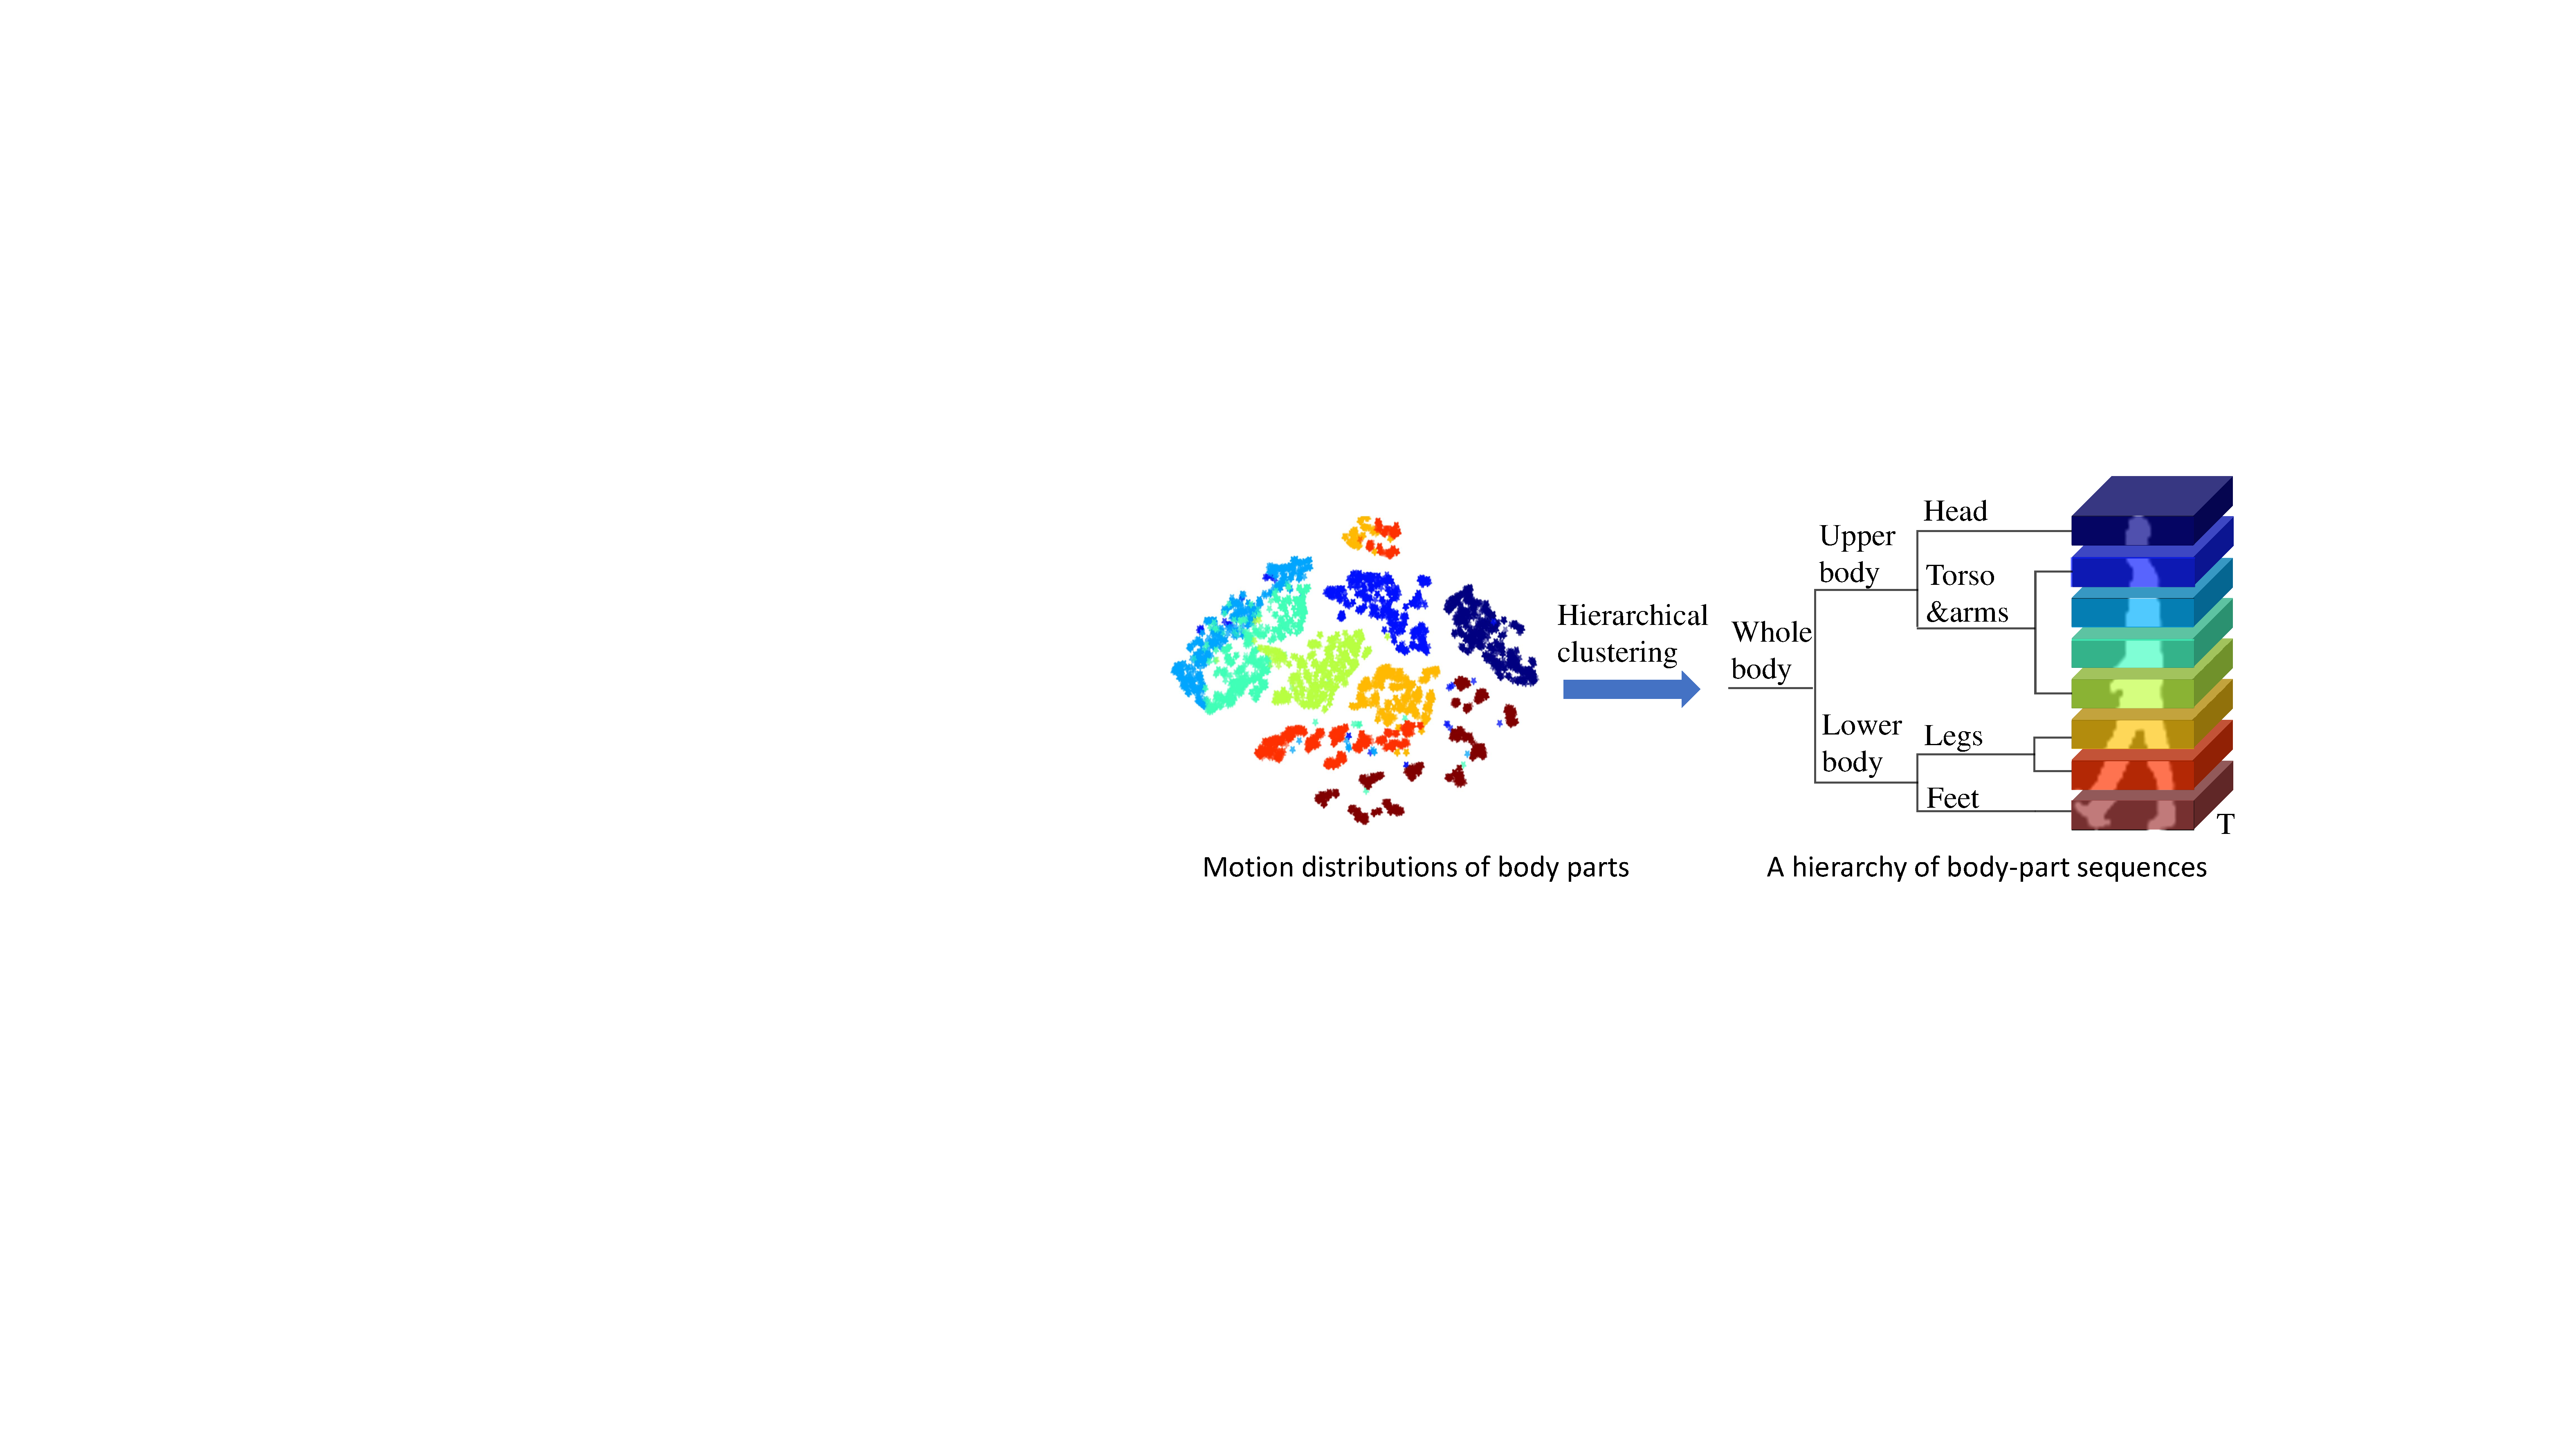
\includegraphics[width=1.0\linewidth]{motivation3.pdf}
\caption{The motivation for our approach. Left: the motion distributions of body parts. The same color indicates the same spatial location across multiple gait sequences in the CASIA-B dataset. Right: an example hierarchy of body-part sequences where $T$ denotes the temporal dimension of the sequence.}
\label{fig:moti}
\end{figure}

To address these issues, various approaches have been proposed for extracting gait features from silhouette sequences \cite{chao2019gaitset,lin2021gaitmask,huang20213d,huang2021context,zhang2021cross}, 3D human structures \cite{an2020performance,li2020end,teepe2021gaitgraph,zheng2022gait,li2021end}, or gait templates \cite{han2005individual,shiraga2016geinet,yu2017invariant}.
 Silhouette-based gait recognition methods have gained increasing attention due to the ease of obtaining silhouettes from raw videos while preserving essential temporal information. The alignment of the input silhouette makes it possible for some methods to extract local body features by horizontally slicing the silhouette image \cite{zhang2019cross} or intermediate-layer features \cite{fan2020gaitpart,lin2021gait}. This partitioning strategy,  first introduced in person re-identification (ReID) \cite{sun2018beyond}, has been proven to be effective for gait recognition \cite{chao2019gaitset,fan2020gaitpart,hou2020gait,chai2022lagrange}.


However, the main limitation of the above part-based approaches is that they do not consider the hierarchical nature of local body movements \cite{bideau2018best}. For instance, within a gait cycle, the feet and lower body have distinct motion characteristics. Therefore, it is important to treat these body regions separately and investigate their part-whole relationships. Our motivation stems from the examination of body-part-specific motion clues. Specifically, each raw gait sequence in the CASIA-B \cite{yu2006framework} dataset is uniformly divided into eight part sequences along the body axis, so that each division roughly match a particular body part \footnote{Each part is pooled into a vector for visualization using t-SNE \cite{van2008visualizing}.}. The distributions of all body parts are shown in the left part of Fig.~\ref{fig:moti}. Observably, some parts, e.g., the head and feet, are easily separated owing to their large changes in walking kinematics. Whereas other parts, such as the thighs and calves, overlap due to the strong motion correlations between them. Further, to identify the relational structure among the part sequences, a hierarchical clustering analysis \cite{ester1996density} is performed. The results are shown in the right part of Fig.~\ref{fig:moti}, indicating that the semantic body regions can be captured in the higher clustering levels without precise localization of the body parts.


Following the above findings, we propose a novel hierarchical spatio-temporal representation learning (HSTL) framework for gait representation. The HSTL framework consists of multiple adaptive region-based motion extractor (ARME) modules, which are stacked to learn hierarchical motion patterns implied in a gait sequence (as shown in Fig.\ref{fig:moti}). In the ARME module, to account for inter-regional differences, non-shared 3D convolutions are used in correspondence with individual body regions. There regions are pre-identified by a hierarchical clustering process performed on fixed horizontal partitions, allowing each body region to cover one or more body parts.  Consequently, the deeper the ARME is, the more local features it tends to extract. Moreover, an adaptive spatio-temporal pooling (ASTP) module is proposed, which couples with an ARME module on the corresponding level to obtain hierarchical gait embeddings.



%The HSTL framework stacks multiple designed modules, named adaptive region-based motion extractor (ARME), to learn hierarchical motion patterns implied in a gait sequence (as shown in Fig.\ref{fig:moti}). In ARME, to cater to inter-regional differences, some non-shared 3D convolutions are in one-to-one correspondence with individual body regions. Those regions are pre-identified by a hierarchical clustering process performed on fixed horizontal partitions, allowing each body region to cover one or more body parts. Therefore, the deeper the ARME is, the more local features it tends to extract. Moreover, an adaptive spatio-temporal pooling module (ASTP) is proposed, which couples with an ARME module on the corresponding level to obtain hierarchical gait embeddings.


In addition, changes in gait speed or sampling frequency may result in several redundant frames in a gait sequence. Although several temporal fusion strategies have been proposed, they lose spatial information \cite{fan2020gaitpart,huang2021context} or lack adaptability \cite{lin2021gait,lin2021gaitmask}. To address this issue, we propose a frame-level temporal aggregation strategy (FTA). FTA fuses temporal features at multiple time steps, preserving significant motion information while compressing the sequence length. The main contributions of this paper are summarized as follows.


%Due to changes in gait speed or sampling frequency, there could be several redundant frames in a gait sequence.Although several temporal fusion strategies have been proposed, they lose spatial information\cite{fan2020gaitpart,huang2021context} or lack adaptability\cite{lin2021gait,lin2021gaitmask}. To solve this issue, a frame-level temporal aggregation strategy (FTA) is proposed. FTA fuses temporal features at multiple time steps, which preserves significant motion information while compressing the sequence length. The main contributions of this paper are summarized as follows.

%feature maps of different depths contain different gait details. In order to capture discriminative gait representations, we designed the adaptive spatio-temporal pooling module (ASTP) to aggregate different levels of gait features, performing hierarchical feature mapping instead of traditional feature mapping \cite{chao2019gaitset,fan2020gaitpart,lin2021gait}.








$\bullet$ We propose a hierarchical spatio-temporal representation learning (HSTL) framework for gait recognition. HSTL takes into account the dependencies of body regions in gait motions, ensuring simplicity and scalability of the architectural design.

$\bullet$ We introduce an adaptive region-based motion extractor (ARME) module to learn region-independent spatio-temporal representation for gait sequences, an adaptive spatio-temporal pooling (ASTP) module to perform hierarchical feature mapping, and a frame-level temporal aggregation (FTA) strategy to compress a gait sequence by removing redundant frames.

$\bullet$ Extensive experiments on the widely used gait datasets CASIA-B \cite{yu2006framework}, including OUMVLP \cite{NorikoTakemura2018MultiviewLP}, GREW \cite{zhu2021gait} and Gait3D \cite{zheng2022gait}, demonstrate that our method achieves state-of-the-art performance while offering a suitable trade-off between model accuracy and complexity.



%-------------------------------------------------------------------------
\section{Related Work}
%metagait gaitedge HPM
\label{sec:rela}
\subsection{Gait Recognition} Deep learning-based gait recognition methods can be broadly categorized into two categories: model-based and appearance-based. Model-based approaches extract structure and motion information from gait videos with the aid of pose estimation \cite{an2020performance,li2020end,teepe2021gaitgraph,li2021end,teepe2022towards,zheng2022gait}. Although these methods are robust to changes in viewpoint and appearance, they are sensitive to the accuracy of the pose parameters, making them incapable of handling low-resolution data. On the other hand, appearance-based approaches learn the feature
representation from raw videos \cite{zhang2019gait,song2019gaitnet,liang2022gaitedge}, or binary silhouette sequences \cite{han2005individual,shiraga2016geinet,yu2017invariant,chao2019gaitset,hou2020gait,fan2020gaitpart,hou2021set,lin2021gait,huang20213d,hou2022gait,chai2022lagrange,dou2022metagait}, which offer greater flexibility than model-based approaches. Our proposed method belongs to the family of appearance-based methods and uses silhouette sequences as inputs.
\begin{figure*}[htbp]
  \centering
  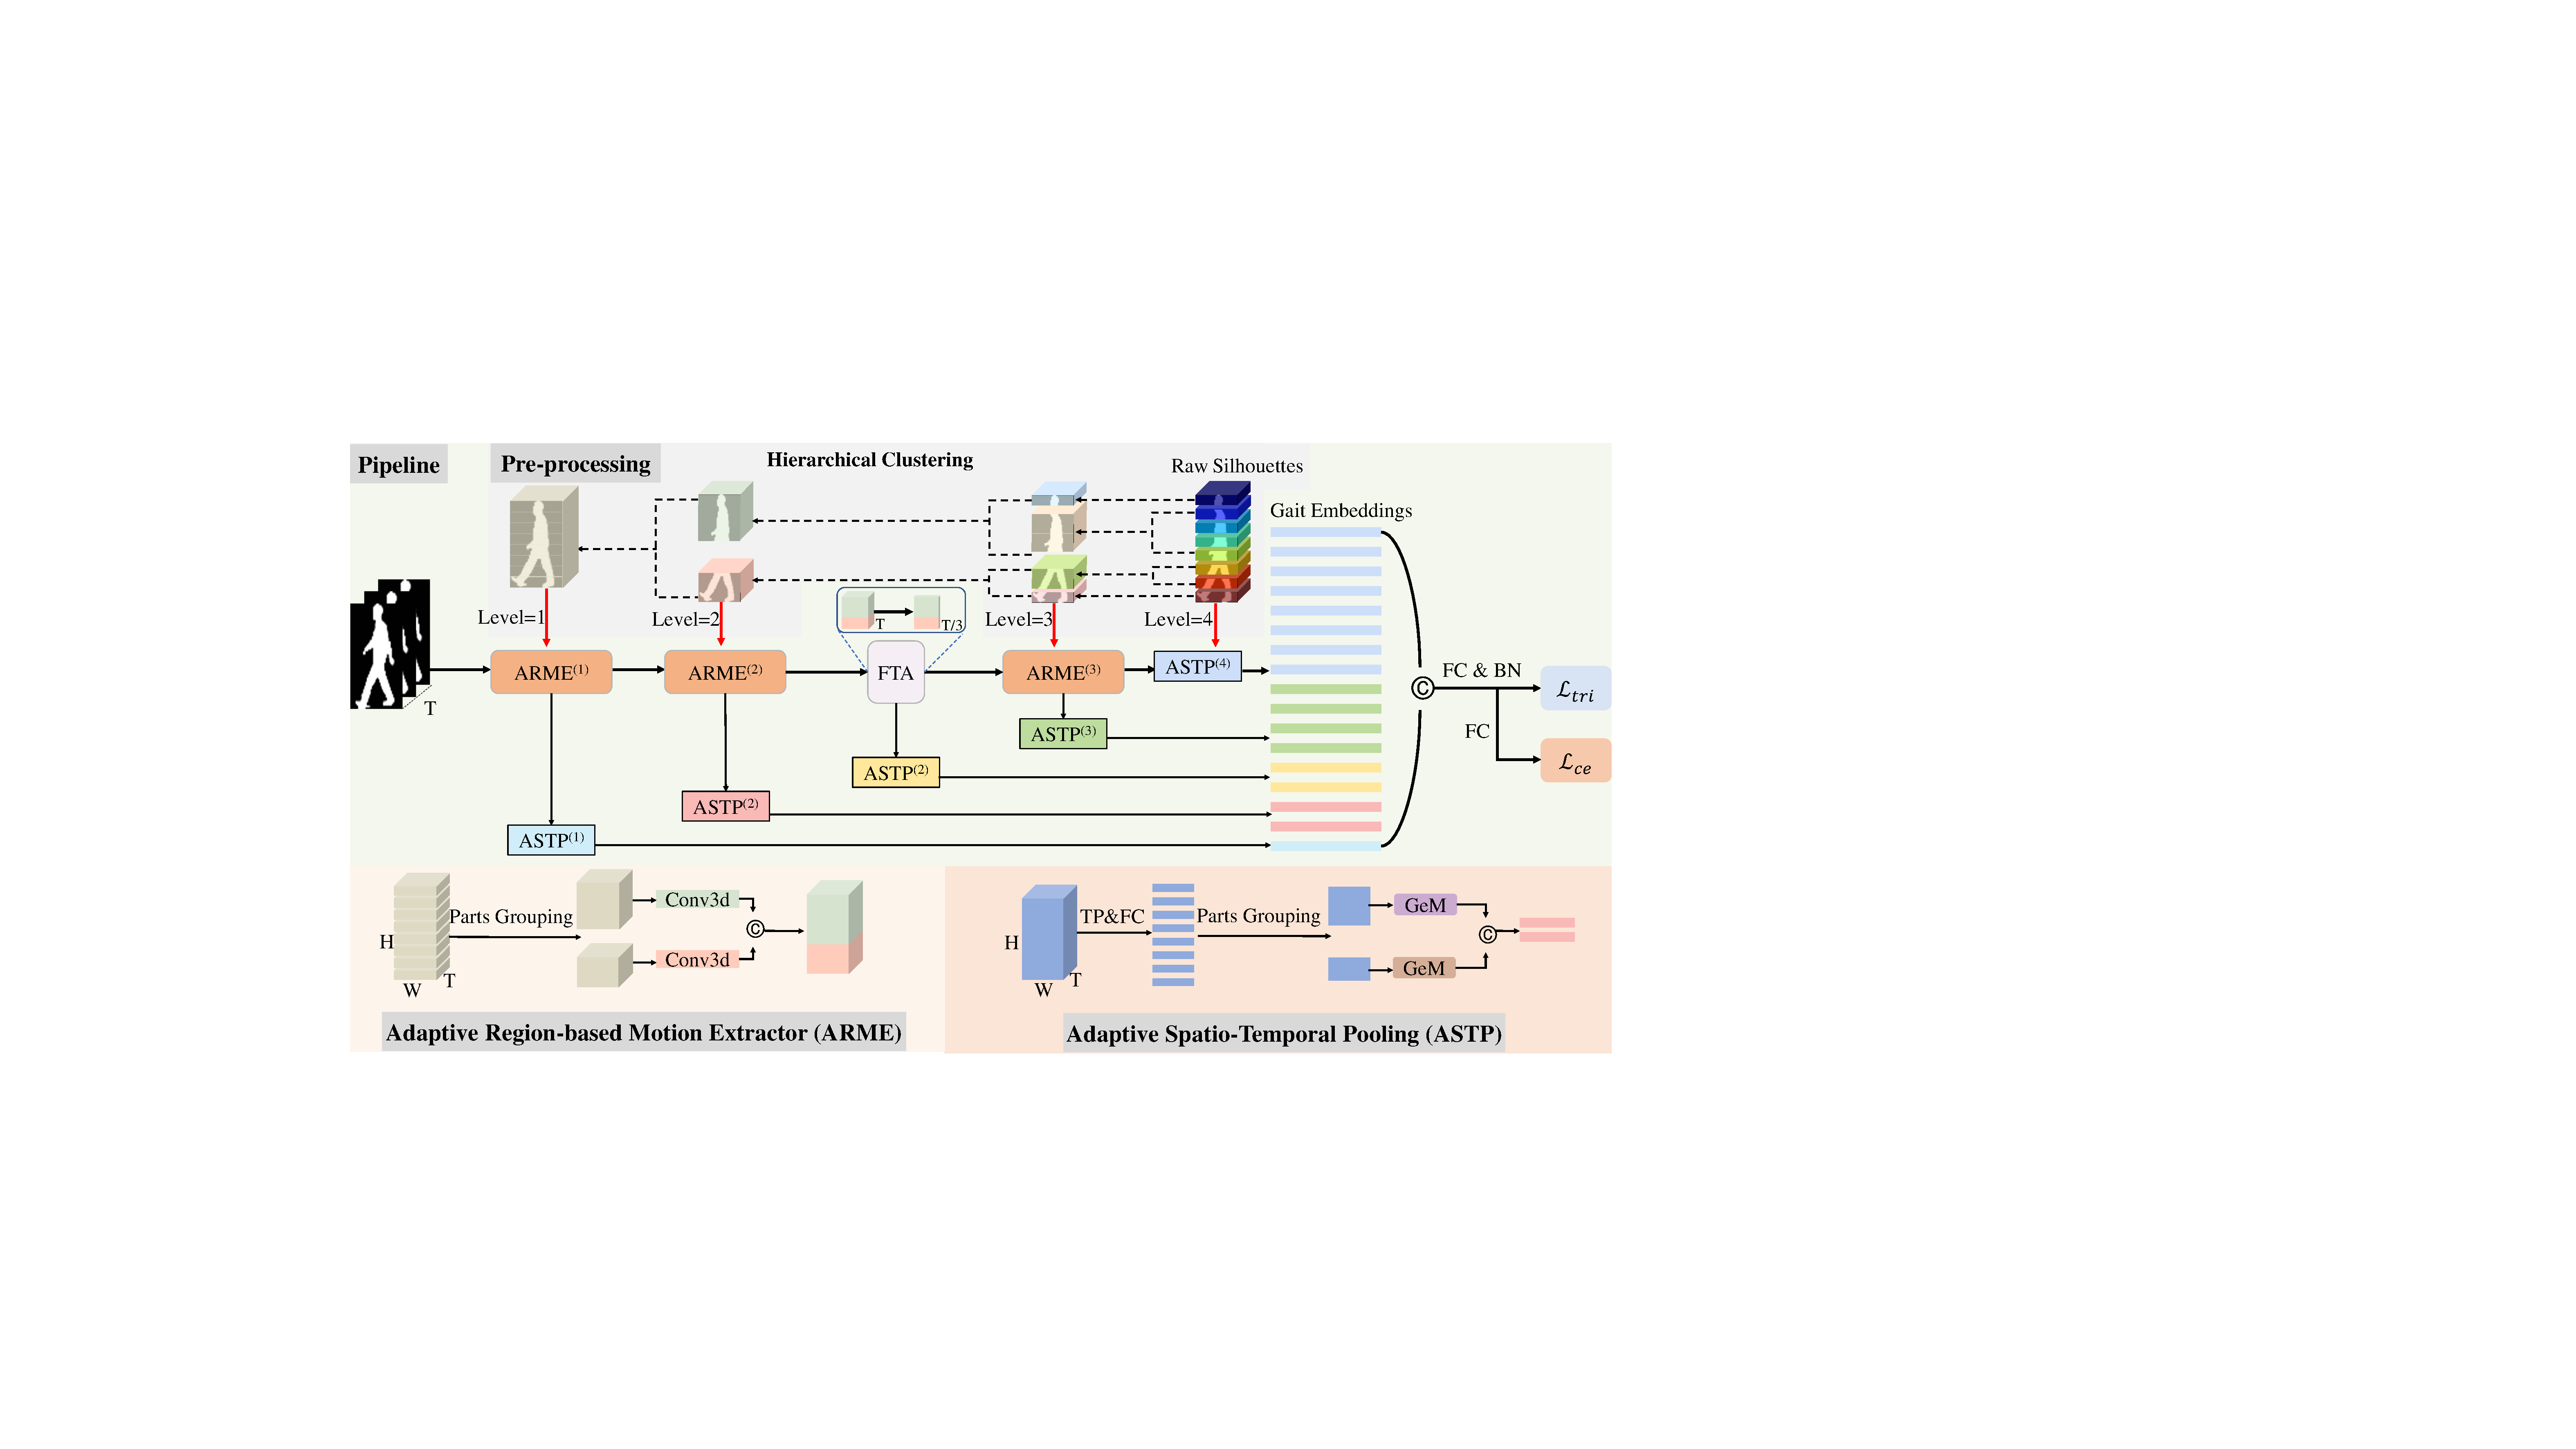
\includegraphics[width=1.00\linewidth]{pyramid.pdf}
\caption{The framework of HFSL. It mainly consists of three modules: ARME (adaptive region-based motion extractor), ASTP (adaptive spatio-temporal pooling), and FTA (frame-level temporal aggregation).  During pre-processing, a hierarchy of walking is obtained to guide the architectural design of HFSL. The framework uses multiple ARMEs to extract gait features from the entire body to individual regions. The ASTP module performs hierarchical feature mapping for the output of each level of ARME. The FTA module compresses local clips of each gait sequence to reduce the number of redundant frames. $T$, $H$ and $W$ denote dimensions of the feature maps. $\copyright$ represents the concatenation operation.}
\label{fig:method}
\end{figure*}

%For simplicity, we omit the channel dimension $C$

\subsection{Hierarchical Model} Hierarchical feature representation has been successfully applied to a wide range of vision tasks. Here, we provide a brief review of the hierarchical object ReID approaches related to gait recognition.

In person ReID, some approaches  \cite{matsukawa2016hierarchical,zhang2022person,wang2021robust,tan2022dynamic,zhang2021coarse} hierarchically learn local descriptions and aggregate appearance features at different levels. For example, Matsukawa \etal \cite{matsukawa2016hierarchical} described an image patch via hierarchical Gaussian distribution. Zhang \etal \cite{zhang2021coarse} proposed a framework to learn coarse-grained and fine-grained features according to body structure. To solve the occlusion problem, Tan \etal \cite{tan2022dynamic} devised a hierarchical mask generator to learn from both occluded and holistic joint images. In vehicle ReID, some approaches \cite{wei2018coarse,shyam2021adversarially,li2022attribute}
extract features from vehicle images in a hierarchical manner. For instance, Wei \etal \cite{wei2018coarse} proposed an RNN-based module for extracting latent cues from the model level to the vehicle level. Shyam \etal \cite{shyam2021adversarially} developed an attention-based hierarchical feature extractor. In addition, Li \etal \cite{li2022attribute} proposed a global structural embedding module for investigating hierarchical relationships between vehicle characteristics by incorporating attribute and state information.

For gait recognition, fusing features of multiple granularities can improve performance \cite{zhang2019cross,fan2020gaitpart,lin2021gait,lin2021gaitmask,huang20213d,chai2022lagrange}. In particular, CSTL \cite{huang2021context} proposed a temporal modeling network that integrates multi-scale temporal features adaptively. By combining part-level and sequence-level features, GaitPart \cite{fan2020gaitpart} obtained a part-independent spatio-temporal expression. Additionally, GaitGL \cite{lin2021gait} considered both full body-based and part-based information to achieve discriminative feature learning. Instead of equally dividing the feature maps, in 3D Local \cite{huang20213d},  a localization operation was developed to find 3D volumes of body parts in a sequence. However, most existing gait recognition methods do not sufficiently exploit the hierarchical dependencies among body parts during walking. In this paper, the proposed HSTL performs a coarse-to-fine hierarchical strategy that integrates multi-level motion patterns from gait sequences.
\subsection{Temporal Model}
%之前的方法专注于步态的空间特征。一些方法为了降低计算代价，将剪影序列直接压缩为1帧。一些方法则直接描述剪影集合中的互补性，认为时间特征并不重要。
Temporal cues play a crucial role in gait recognition due to the periodic changes in body shape. Previous methods treat a gait sequence as an unordered set, either compressing it into a single gait template during preprocessing \cite{shiraga2016geinet,li2020gait} or learning order-independent gait representations from silhouette sets \cite{chao2019gaitset,hou2020gait,hou2021set}. These methods assume that different subjects share similar global gait patterns, making ordering inputs unnecessary for gait assessment. However, ignoring the temporal nature of the gait sequence can result in missing discriminative local motion information. Recently, some approaches have achieved significant performance gains by explicitly modeling temporal information using LSTM \cite{zhang2019cross}, 1D convolution \cite{huang2021context}, and 3D convolution \cite{lin2020gait,huang20213d}. Nevertheless, these spatio-temporal operators also significantly increase computational costs. Although
 some methods have been proposed to reduce video length by aggregating local clips \cite{lin2021gait,lin2021gaitmask,chai2022lagrange}, they lack adaptability to variations in pace. The main difference between our approach and others \cite{li2019selective,hou2021bicnet} is that we employ multi-scale temporal pooling at the frame level while considering variations in motion across body regions, leading to a more adaptable reduction of the gait sequence length.



 %Building on the successful application of multi-scale attention fusion mechanisms in spatial  and temporal \cite{hou2021bicnet} terms. We effectively reducing the sequence length by fusing informative temporal features at multiple time steps in a soft-attention way.
% The main difference between our approach and others is that we perform a multi-scale temporal pooling strategy at the frame level, effectively reducing the sequence length by fusing informative motion features at multiple time steps.
%-------------------------------------------------------------------------
\section{Proposed Method}
\label{sec:method}
In this section, we present the detailed description of HSTL, including the adaptive region-based motion extractor (ARME), the adaptive spatio-temporal pooling (ASTP), and the frame-level temporal aggregation (FTA).



\subsection{Framework Pipeline}
\label{sec:pipe}
The overview of our HSTL is presented in Fig.~\ref{fig:method}. Given a gait dataset $\mathcal{D}=\{{S_i}\}_{i=1}^{N} $ with $N$ gait sequences, where each sequence $S_i \in \mathbb{R}^{C \times T \times H \times W}$ is represented as a 4D tensor with $C$ channels, $T$ frames, and $H \times W$ pixels. During  the preprocessing stage, each gait sequence $S_i$  is divided horizontally and uniformly into $k$ part sequences, indexed from 1 to $k$. Then, a hierarchical clustering algorithm \cite{ester1996density} is applied to these part sequences to obtain a generic hierarchy of gait motions, which is denoted as $\mathcal{P}=\{\mathcal{P}^{(l)}\}_{l=1}^{L}$. Here, $L$ is the number of levels in the hierarchy and $\mathcal{P}^{(l)}$ is the set of partitions at level $l$. The partitions at level $l$ are defined as
 $\mathcal{P}^{(l)}=\{P_1^{(l)}, P_2^{(l)}, \ldots, P_{K_{l}}^{(l)}\}$, where $P_j^{(l)}$ is the $j$-th subset of part indices and $K_l$ is the number of groups at level $l$. For instance, the top level $\mathcal{P}^{(1)}=\left\{\{1,2,\ldots, k-1,k\}\right\}$ means all the $k$ parts can be considered as a whole for the gait analysis. This hierarchy provides a structured  property of the gait motion patterns and can be utilized to guide gait feature extraction. To achieve this, our proposed HSTL employs three modules: ARME for extracting independent multi-granularity motion features, ASTP for generating vectorized gait embeddings, and FTA for reducing redundant information at the frame level. The HSTL stacks these three modules according to the division in $\mathcal{P}$, and the main branch of the HSTL for the input sequence $S_{in}$ can be formalized as:
\begin{equation}
\label{eq:pipeline}
    Y^{M}=\Gamma^{(L)} \circ \Psi^{(L-1)} \circ \cdots \circ \Omega^{(2)} \circ \Psi^{(2)} \circ \Psi^{(1)}(S_{in}),
\end{equation}
where $\Psi^{(l)}$, $\Gamma^{(l)}$, and $\Omega^{(l)}$ represent the ARME, ASTP and FTA modules at the $l$-th level of $\mathcal{P}$, respectively.  Since FTA uses inter-frame compression to reduce redundant information, it is employed only once at the $l_{\Omega}$-th level in $\mathcal{P}$ (e.g., $l_{\Omega}=2$ in Eq. (\ref{eq:pipeline})) to prevent excessive loss of information.





To obtain the hierarchical gait embeddings, the output $Y^{(l)}$ of each $\Psi^{(l)}$ at levels $l \in \{1, 2, \ldots, L-1\}$ and the output of $\Omega^{(l_{\Omega})}$ at level $l_{\Omega}$, denoted as $Y_{\Omega}^{(l_{\Omega})}$,  are fed into the corresponding $\Gamma^{(l)}$. The resulting outputs from these $L$ auxiliary branches are concatenated with the output of the main branch defined in Eq.~(\ref{eq:pipeline}), forming the final result, denoted as $Y$, which is given by:
\begin{align}
  Y =  \biggl[ & Y^{M}, \Gamma^{(L-1)}\left(Y^{(L-1)}\right),  \ldots , \nonumber \\
  & \Gamma^{(l_{\Omega})}\left(Y_{\Omega}^{(l_{\Omega})}\right), \Gamma^{(2)}\left(Y^{(2)}\right), \Gamma^{(1)}\left(Y^{(1)}\right) \biggl],
\end{align}
where $[,]$ denotes the concatenation operation.




%一个级联多个ARME，做层次化的动作特征提取。 一个堆叠ARSP做层次化的时空信息聚合。再一个就是时间维度下采样。


% $$
% P^{(i)}=\left\{P_1^{(i)}, P_2^{(i)}, \ldots, P_{K_{i}}^{(i)}\right\}
% $$
% ARME$^{(i)}$
% $\Psi^{(i)}$



%The overview of our HSTL is presented in Fig.~\ref{fig:method}. In the pre-processing phase, a hierarchical clustering method \cite{ester1996density} is used to build a pyramid structure of body motions. Specifically, we slice the silhouette sequence $S \in \mathbb{R}^{C \times T \times H \times W}$ into $k$ part-sequences on height, denoted as $S_{part}=\left\{S_i \mid i=1,2,\cdots, k\right\}$. $S_i \in \mathbb{R}^{C \times T \times \frac{H}{k} \times W}$ corresponds to the i-th part-sequence. $C$ is the number of channels, $T$ is the length of sequence and $(H,W)$ is the silhouette size.  Then, depending on the similarity of the distributions of $S_{part}$, $S_i$ is iteratively merged into groups. Thus, we can obtain the clustering results $I^{(l)}=\left\{I^{(l)}_g \mid g=1,2,\cdots,G_l\right\}$, after parts grouping, where $l \in 1,2,\cdots,L$, $l,g$ stand for the index of level and the index of groups, $L$ is the number of levels and $G_l$ is the number of groups for the $l$-th level.
%, where $n \in 1,2,\cdots,N$. For example, when $k=8,l=2,N=2$. The $N$ grouped part-sequences $V_{l,1}=[v_1,\cdots,v_5] \in \mathbb{R}^{C \times T \times \frac{5}{8}H \times W}$ and $V_{l,N}=[v_6,\cdots,v_{k}] \in \mathbb{R}^{C \times T \times \frac{3}{8}H \times W}$, where $\left[\cdot\right]$ represents the concatenation operation on height.

% % Table generated by Excel2LaTeX from sheet 'Sheet1'
% \begin{table}[htbp]
%   \centering
%   \caption{Add caption}
%     \begin{tabular}{c|c}
%     \toprule
%     Level & Parts Grouping \\
%     \hline
%     1     & $[v_0,\cdots,v_7]$ \\
%     % \midrule
%     2     & $[v_0,\cdots,v_4],[v_5,\cdots,v_7]$ \\
%     % \midrule
%     3     & $[v_0],[v_1,\cdots,v_4],[v_5,v_6],[v_7]$ \\
%     \bottomrule
%     \end{tabular}%
%   \label{tab:addlabel}%
% \end{table}%



%Then, depending on the similarity of the distributions of $V$, $v_i$ is iteratively merged until the value of groups is one. Finally, the first layer is aggregated into four groups, denoted as $\left\{[v_0],[v_1,\cdots,v_4],[v_5,v_6],[v_7]\right\}$. The second layer is aggregated into two groups, denoted as $\left\{[v_0,\cdots,v_4],[v_5,\cdots,v_7]\right\}$. The third layer is aggregated into one group, denoted as $\left\{[v_0,\cdots,v_7]\right\}$, where $\left[\cdot\right]$ represents the concatenation operation on height.
% Given a sequence $S_{in}  \in \mathbb{R}^{C \times T \times H \times W}$ as the input of HSTL. First, the feature of $S_{in}$ for the $l$-th ARME can be formulated as:

% \begin{equation}
%     \mathbf{F}^{(l)}=\text{ARME}^{(l)}\left(S_{in};\mathcal{W}^{(l)}\right),
% \end{equation}

% where $\text{ARME}^{(l)}:\mathbb{R}^{C \times T \times H \times W} \mapsto \mathbb{R}^{C_l \times T \times H \times W}$ parameterized by a set of trainable parameters $\mathcal{W}^{(l)}$, $l \in \left\{1,2,\cdots,L-1\right\}$. Secondly, feature mapping is performed for the output of each level of ARME, denoted as
% \begin{equation}
%     \begin{aligned}
%         \mathbf{F}_{out1} &= f_{sfs}\left(\left[\text{ASTP}^{(l)}\left(\mathbf{F}^{(l)}\right)\right]\right),\\
%         \mathbf{F}_{out2} &= f_{sfs}\left(\text{ASTP}^{(L)}\left(\mathbf{F}^{(L-1)}\right)\right),\\
%         \mathbf{F}_{out} &= \left[\mathbf{F}_{out1}, \mathbf{F}_{out2}\right]
%     \end{aligned}
% \end{equation}
% where $f_{sfs}\left(\cdot\right)$ denotes the multiple separate fully connected layers, $\left[\cdot\right]$ represents the concatenation operation on height, $\mathbf{F}_{out} \in \mathbb{R}^{C_{L-1} \times \sum_{l=1}^{l=L}G_l}$ is the output of feature mapping. Furthermore, FTA can add after the $l$-th ARME, denoted as
% \begin{equation}
%     \mathbf{F}_{fta} = \text{FTA}\left(\mathbf{F}^{(l)}\right),
%     \label{label:lta}
% \end{equation}
% where $\mathbf{F}_{fta} \in \mathbb{R}^{C_l\times \frac{T}{3} \times H \times W}$ is the output of FTA.




Finally, $Y$ undergoes feature mapping through separate fully connected layers. The model is then trained using a combination of triplet loss $\mathcal{L}_{tri}$ and cross-entropy loss $\mathcal{L}_{ce}$, which is a commonly adopted practice in gait recognition \cite{hou2020gait,lin2021gait,huang2021context,huang20213d,dou2022metagait}.  Further details regarding the relevant modules are described in the following subsections.


%Finally, we train the model using a combination of triplet $\mathcal{L}_{tri}$ and cross-entropy $\mathcal{L}_{ce}$ losses, which are commonly used for gait recognition .

% The feature representation of $S_{in}$ at the $l$-th level of detail can be denoted as
% \begin{equation}
%     \mathbf{F}_{l} = \Psi_l\left(S_{in}\right),
% \end{equation}
% where $\Psi_l \left(\cdot\right)$ represents the ARME for the $l$-th level. $\mathbf{F}_{l} \in \mathbb{R}^{C_l\times T \times H \times W}$ is the output of $\Psi_l \left(\cdot\right)$. Furthermore, when $l=2$, we add a FTA module after $l$-th ARME. The process can be formulated as
% \begin{equation}
%     \mathbf{F}_{fta} = \mathcal{P}\left(\mathbf{F}_{l}\right),
% \end{equation}
% where $\mathcal{P}\left(\cdot\right)$ represents the FTA module. $\mathbf{F}_{fta} \in \mathbb{R}^{C_l\times \frac{T}{3} \times H \times W}$ is the output of $\mathcal{P}\left(\cdot\right)$. Next, the ASTPs are added to the output of each ARME  and the output of FTA to perform a hierarchical feature mapping, which is then concatenated on height to obtain the representations used for recognition.

% Next, after frame compression by FTA module, the output feature map $\mathbf{F}_{fe} \in \mathbb{R}^{C_out\times \frac{T}{3} \times H \times W}$ of the $\text{ARME}_l$is converted into a spatio-temporal feature that can describe the gait, denoted as
% \begin{equation}
%     \mathbf{F}_{fe}=\Psi_3\circ\Gamma \circ\Psi_2\circ\Psi_1\left(S_{in}\right),
% \end{equation}
% where $\mathbf{F}_{fe} \in \mathbb{R}^{C_out\times \frac{T}{3} \times H \times W}$ is the output of $\Psi_3\left(\cdot\right)$. The $\Psi_i\left(\cdot\right)$ represents the ARME for the $l$-th level and ARME will be described in Sec.~\ref{sec:pyra}. $\Gamma\left(\cdot\right)$ represents the FTA, which will be described in Sec.~\ref{sec:multi}. Next, the ASTP is added to the output of each ARME to perform a hierarchical feature mapping, which is then concatenated on height to obtain the representations used for recognition. Finally, we train the model using a combination of triplet $L_{tri}$ and cross-entropy $L_{ce}$ losses, which are commonly used for gait recognition \cite{hou2020gait,lin2021gait,huang2021context,huang20213d,dou2022metagait}.

% Then, since $\mathbf{F}_{fe}$ is still a high-dimensional feature, Temporal Pooling  (TP) \cite{fan2020gaitpart,lin2020gait,lin2021gait,lin2021gaitmask} is used to aggregate the temporal-dynamic information of the whole sequence. Later the spatial information is mapped to the discriminant space by Generalized Mean pooling (GeM) \cite{lin2021gait,lin2021gaitmask}. Finally, the network is trained jointly using cross-entropy loss and triplet loss. The details will be described in Sec.~\ref{sec:loss}.

\subsection{Adaptive Region-based Motion Extractor}
\label{sec:pyra}

The adaptive region-based motion extractor (ARME) aims to extract independent spatio-temporal patterns that are associated with different human body parts in a gait sequence. Unlike existing methods that uniformly slice gait images or sequences along the height axis \cite{zhang2019cross,fan2020gaitpart,lin2021gait,lin2021gaitmask}, ARME considers the inherent hierarchical relationships among different part sequences that are consistent with walking patterns. This allows ARME to effectively capture the unique walking kinematics of each part.

%Given the hierarchical relation $\mathcal{P}$ introduced in Section \ref{sec:pipe}, the corresponding
%ARME module $\Psi^{(l)}$ for the $l$-th level partition $\mathcal{P}^{(l)}$ is defined as follows:
Given the hierarchical relation $\mathcal{P}$ introduced in Section \ref{sec:pipe}, ARME first divides the input sequence $X$ into $K_l$ regions based on the partition of the $l$-th level $\mathcal{P}^{(l)}$, resulting in the set of regions $\{X_{j}^{(l)}\}_{j=1}^{K_l}$, where $X_{j}^{(l)} \in \mathbb{R}^{C \times T \times H_j^{(l)} \times W}$. $H^{(l)}_j=\frac{\left|P_j^{(l)}\right|}{k}H$ is the height of the $j$-th region of the $l$-th level. Then the $l$-th level of ARME, $\Psi^{(l)}$, can be defined as follows:
\begin{equation}
    Y^{(l)}_{\Psi}=\Psi^{(l)}(X^{(l)})=\left[f_{1}(X_{1}^{(l)}), f_{2}(X_{2}^{(l)}) ,\ldots, f_{K_l}(X_{K_l}^{(l)})  \right],
\end{equation}
where $f_{j}\left(\cdot\right)$ represents the independent 3D convolution operation applied to the $j$-th region. The output feature map $Y^{(l)}_{\Psi} \in \mathbb{R}^{C^{(l)} \times T \times H \times W}$ of level $l$ has $C^{(l)}$ channels. This module only modifies the number of channels, preserving the spatial and temporal resolutions of the input feature map.


%$Y^{(l)} \in \mathbb{R}^{C^{(l)} \times T \times H \times W}$ is the output feature map, and $C^{(l)}$ denotes the number of output channel of level $l$.  By default, this module only changes the number of channels, while preserving the spatial and temporal resolution.


%The ARME is shown in Fig.~\ref{fig:method}. Given the input $S_i=\{X_{i,j}^{(l)}\}_{j=1}^{K_l}$ of ARME. Then the $l$-th level of ARME, $\Psi^{(l)}$, can be defined as follows:
% \begin{equation}
%     \Psi^{(l)}(S_i)=\left[\text{Conv3D}(S_{i,1}^{(l)}), \text{Conv3D}(S_{i,2}^{(l)}) \ldots \text{Conv3D}(S_{i,K_l}^{(l)})  \right]
% \end{equation}





% The ARME is shown in Fig.~\ref{fig:method}, ARME uses the parts grouping opposite to the pre-processing process in Sec~\ref{sec:pipe} to extract the gait features from coarse to fine.
%The adaptive region-based motion extractor (ARME) aims to extract independent spatio-temporal patterns associated with human body parts in the temporal variation of the sequence, and it is a novel operation developed for gait data based on a component constructed by 3D convolution. First, it performs horizontal splits along the height dimension of the input feature map, which is common in \cite{zhang2019cross,fan2020gaitpart,lin2021gait,lin2021gaitmask}. The difference is that based on the group manner obtained in the pre-processing phase of Sec.~\ref{sec:pipe}, we split the feature map horizontally but not uniformly. Standard 3D convolution operations are then performed on the spatio-temporal features of each part sequence. Note that the parameters are non-shared between these convolution operations.

%The ARME is shown in Fig.~\ref{fig:method}. Assume that the input of ARME is $\mathbf{F} \in \mathbb{R}^{C \times T \times H \times W}$, first, we split $\mathbf{F}$ into $k$ parts, denoted as $\mathbf{F}_{part}=\left\{\mathbf{F}_i \mid i=1,2,\cdots, k\right\}$, where $\mathbf{F}_i\in\mathbb{R}^{C \times T \times \frac{H}{k} \times W}$. According the parts grouping results $I^{(l)}$ in Sec.~\ref{sec:pipe}, grouping $\mathbf{F}_{part}$, we can obtain the features $\mathbf{F}^{(l)}=\left\{\mathbf{F}^{(l)}_g \mid g=1,2,\cdots,G_l\right\}$. Secondly, the process of spatio-temporal feature extractor for the $l$-th level can be formulated as
% \begin{equation}
%     \mathbf{F}_{arme}^{(l)}=\left[f_{conv3d,g}\left(\mathbf{F}^{(l)}_g \right)\right]
% \end{equation}
% where $f_{conv3d,g}\left(\cdot\right)$ represents the 3D convolution operation. $\mathbf{F}_{arme}^{(l)} \in \mathbb{R}^{C_l \times T \times H \times W}$ is the output of the $l$-th level ARME.
% Note that the $f_{conv3d}^g\left(\cdot\right)$ used for each $\mathbf{F}^{(l)}_g$ is separate.
% For example, when $k=8,l=2,N=2$. The $N$ grouped part-features $\mathbf{F}_{l,1}=[\mathbf{f}_1,\cdots,\mathbf{f}_5] \in \mathbb{R}^{C \times T \times \frac{5}{8}H \times W}$ and $\mathbf{F}_{l,N}=[\mathbf{f}_6,\cdots,\mathbf{f}_{k}] \in \mathbb{R}^{C \times T \times \frac{3}{8}H \times W}$. Secondly, the independent 3D convolution operation is performed for each part-features, denoted as
% \begin{equation}
%     \begin{split}
%         \mathbf{F}_{arme}^{1}=f_{conv3d}\left(\mathbf{F}_{l,1}\right) \in \mathbb{R}^{C_1 \times T \times \frac{5}{8}H \times W},\\
%         \mathbf{F}_{arme}^{N}=f_{conv3d}\left(\mathbf{F}_{l,N}\right) \in \mathbb{R}^{C_1 \times T \times \frac{3}{8}H \times W},
%     \end{split}
% \end{equation}
% Note that the 3D convolution can have a layer or multiple layers.
% Finally, the $\mathbf{F}_{arme}^{1}$ and $\mathbf{F}_{arme}^{N}$ are concatenated on height, and the process can be formulated as
% Thus we can obtained the output feature maps $\mathbf{F}_{arme}^{1} \in \mathbb{R}^{C_1 \times T \times \frac{5}{8}H \times W}$ and $\mathbf{F}_{arme}^{2} \in \mathbb{R}^{C_1 \times T \times \frac{3}{8}H \times W}$. Finally, the feature maps are concatenated on height, denoted as
% \begin{equation}
%     \mathbf{F}_{arme} = \left[\mathbf{F}_{arme}^{1}, \mathbf{F}_{arme}^{N}\right],
% \end{equation}
%其中$\mathbf{F}_{pcb} \in \mathbb{R}^{C_1 \times T \times H \times W}$是PCB操作的输出特征图。
% where $\mathbf{F}_{arme} \in \mathbb{R}^{C_1 \times T \times H \times W}$ is the output of ARME.

\subsection{Adaptive Spatio-Temporal  Pooling}
\label{sec:astp}
%传统的特征聚合\cite{chao2019gaitset,lin2020gait,lin2021gait,lin2021gaitmask,huang20213d,huang2021context}首先将特征图平均分成条状，然后以同样的方式降样。相比之下，自适应时空集合（ASTP）旨在聚集与身体部位相关的特征。因此，我们根据在Sec.~ref{sec:pipe}的预处理阶段得到的分组方式对条带进行分组，然后对每组进行单独处理，以获得更具判别性的特征表示。%此外，上述方法聚合靠近输出层特征图来获得步态表征,忽略了网络不同深度的层次信息，我们认为这限制了步态识别的性能。值得注意的是，ASTP采用类似TesNet和DenseNet类似的跳连操作，利用了每个ARME生成的输出，从而改善了特征表征能力。

It is a common procedure in gait recognition to obtain a compact and fixed-length feature representation by performing horizontal and uniform slicing of feature maps and strip-based pooling \cite{chao2019gaitset,fu2019horizontal,lin2020gait,lin2021gait,huang2021context}. However, a non-uniform division of the feature maps is better at capturing the gait motion characteristics. Thus, the adaptive spatio-temporal pooling (ASTP) is devised to construct hierarchical feature mapping (as shown in Fig.~\ref{fig:method}). Similar to the ARME module described in Section \ref{sec:pyra}, the hierarchy $\mathcal{P}$ enables us to obtain the $j$-th region of the $l$-th level, denoted as $X_j^{(l)}$. The corresponding ASTP, denoted as $\Gamma^{(l)}$, can be expressed as follow:
\begin{equation}
Y_{\Gamma,j}^{(l)}=\Gamma_j^{(l)}(X_j^{(l)})=\text{GeM}_j \circ \text{FC} \circ \text{Max}(X_j^{(l)}),
\end{equation}
where $\text{Max}(\cdot)$ represents a max pooling operation along the temporal dimension, $\text{FC}(\cdot)$ represents a fully connected layer, $\text{GeM}_j(\cdot)$ represents a generalized mean pooling (GeM) operation \cite{radenovic2018fine} for $j$-th region, and $\Gamma_j:\mathbb{R}^{C \times T \times H_j^{(l)} \times W} \mapsto \mathbb{R}^{C \times 1 \times H_j^{(l)} \times W} \mapsto \mathbb{R}^{C^{(l)} \times 1 \times H_j^{(l)} \times W} \mapsto \mathbb{R}^{C^{(l)} \times 1 \times 1 \times 1}$. Therefore, by concatenating outputs of $K_l$ regions, we can obtain $Y_{\Gamma}^{(l)}=\left[Y_{\Gamma,1}^{(l)},Y_{\Gamma,2}^{(l)},\ldots,Y_{\Gamma,K_l}^{(l)}\right]$, where $Y_{\Gamma}^{(l)} \in \mathbb{R}^{C_{}^{(l)}\times 1 \times  K_l \times 1}$ is the output of ASTP at level $l$.



%Traditional feature aggregation \cite{chao2019gaitset,fu2019horizontal,lin2020gait,lin2021gait,lin2021gaitmask,huang20213d,huang2021context} first splits the feature map equally into strips and then downsamples in the same way. In contrast, adaptive spatio-temporal pooling (ASTP) aims to aggregate features related to body parts. Therefore, we group the strips according to the grouping manner obtained in the pre-processing phase of Sec.~\ref{sec:pipe}, and then process each group individually to obtain more discriminative feature representations. In addition, the above methods aggregate close the output layer feature maps to obtain gait representations, it ignores the hierarchical information at different depths of the model, which we believe limits the performance of recognition. Notably, ASTP uses the skip-connect operations (like ResNet \cite{he2016deep} and DenseNet \cite{huang2017densely}) to exploit the output generated by each ARME, thus improving the feature representation ability.




%
% We next group the strips. Here as an example in two groups, described according to Sec.~\ref{sec:pipe}. Thus, we obtain $\mathbf{F}_{group}^{1} =\left[\mathbf{F}_{split}^{0},\cdots,\mathbf{F}_{split}^{4}\right]\in \mathbb{R}^{C_{3} \times 1 \times \frac{5}{8}H \times W}$ and $\mathbf{F}_{group}^{2}=\left[\mathbf{F}_{split}^{5},\cdots,\mathbf{F}_{split}^{7}\right] \in\mathbb{R}^{C_{3} \times 1 \times \frac{3}{8}H \times W}$.

% Given the input $X=\{X_{j}^{(l)}\}_{j=1}^{K_l}$ of ASTP.
%The ASTP is shown in Fig.~\ref{fig:method}. Given the hierarchical relation $\mathcal{P}$ introduced in Section \ref{sec:pipe}, ASTP first divides the input sequence $X$ into $K_l$ regions based on the partition of the $l$-th level $\mathcal{P}^{(l)}$, resulting in the set of regions $\{X_{j}^{(l)}\}_{j=1}^{K_l}$. Then the $j$-th output region feature for the $l$-th level of ASTP, $Y_{astp,j}^{(l)}$, can be defined as follows:




%where $\text{TP}\left(\cdot\right)$ represents the temporal pooling (TP) \cite{lin2020gait} operation, $\text{FC}\left(\cdot\right)$ represents the fully connected layer, $\text{GeM}_j\left(\cdot\right)$ represents the GeM \cite{lin2021gait,lin2021gaitmask} operation for spatial dimension applied to the $j$-th region feature. $Y_{astp,j}^{(l)}\in \mathbb{R}^{C_{L-1} \times 1}$ is the output after GeM. Finally, each $Y_{astp,j}^{(l)}$ is concated on height, we can obtain $Y^{(l)}=\left[Y_{astp,j}^{(l)}\right]$, where $Y^{(l)} \in \mathbb{R}^{C_{L-1} \times K_l}$ is the output of ASTP.
% The ASTP is shown in Fig.~\ref{fig:method}, assume that the output after the $l$-th level ARME is $\mathbf{F} \in \mathbb{R}^{C_l \times T \times H \times W}$. To obtain sequence-level features, we introduce temporal pooling (TP) \cite{lin2020gait} to aggregation temporal information. TP can be formulated as
% % \begin{equation}
% %     \mathbf{F}_{tp}=\text{Max}\left(\mathbf{F}\right),
% % \end{equation}
% where $\mathbf{F}_{tp} \in \mathbb{R}^{C_l \times 1 \times H \times W}$ is the output of TP. Next, $\mathbf{F}_{tp}$ changes the number of channels via a fully connected layer to obtain the feature $\hat{\mathbf{F}}_{tp} \in \mathbb{R}^{C_{L-1} \times 1 \times H \times W}$. Then we split $\hat{\mathbf{F}}_{tp}$ into $k$ strips, denote as $\mathbf{F}_{strip}=\left\{\hat{\mathbf{F}}_{tp,i} \mid i=1,2,\cdots, k\right\}$, where $\hat{\mathbf{F}}_{tp,i} \in \mathbb{R}^{C_{L-1} \times 1 \times \frac{H}{k} \times W}$. According the parts grouping results $I^{(l)}$ in Sec.~\ref{sec:pipe}, grouping $\mathbf{F}_{strip}$, we can obtain the features $\hat{\mathbf{F}}^{(l)}_{tp}=\left\{\hat{\mathbf{F}}^{(l)}_{tp,g} \mid g=1,2,\cdots,G_l\right\}$. Finally, the spatial information aggregation can be represented as

% where $\mathbf{F}_{astp}^{(l)} \in \mathbb{R}^{C_{L-1} \times 1 \times G_l \times 1}$ is the output of ASTP for the $l$-th level.
% Note that the $\text{GeM}\left(\cdot\right)$ for each $\hat{\mathbf{F}}^{(l)}_{tp,g}$ is separate.
% The $\mathbf{F}_{astp}^{1}$ and $\mathbf{F}_{astp}^{2}$ are concatenated on height, and the process can be formulated as:
% \begin{equation}
%     \mathbf{F}_{astp}=\left[\mathbf{F}_{astp}^{1},\mathbf{F}_{astp}^{2}\right],
% \end{equation}
% where


%Assume

\subsection{Frame-level Temporal Aggregation}
\label{sec:multi}

% A gait sequence may contain several redundant frames due to factors such as the acquisition frame rate and pace frequency. To reduce computational costs, some methods compress a gait sequence by aggregating its  local clips \cite{lin2021gait,lin2021gaitmask}. In the proposed frame-level temporal aggregation (FTA), we consider both the gait structure and the multiscale  temporal information.  Given the $l$-level gait region $X_{j}^{(l)}$, we first merge the features of the two temporal scales using the following formula:
% \begin{equation}
% \begin{aligned}
%     U_{j,1}^{(l)}&=\psi_{a \times 1 \times 1}^{3\times 1 \times 1}\left(X_{j}^{(l)}\right),\\
%     U_{j,2}^{(l)}&=\psi_{b \times 1 \times 1}^{3\times 1 \times 1}\left(X_{j}^{(l)}\right),\\
%     \hat{U}_{j}^{(l)}&=U_{j,1}^{(l)}+U_{j,2}^{(l)},
% \end{aligned}
%     % \hat{U}_{j}^{(l)}=U_{j,1}^{(l)}=\sum_{v=1}^{V}\psi_{v}\left(X_{j}^{(l)}\right),v\in \left\{1,2,\cdots,V\right\},
%     \label{equ:poolfeature}
% \end{equation}
% The frame-level temporal aggregation (FTA) compresses local clips through multiple temporal scales. Its main objective is to preserve temporal information discrimination while removing redundant frame features.
% Since humans have different gait speeds or sampling frequencies due to different walking conditions, FTA introduces multi-scale information to mitigate the inconsistency. Although LTA \cite{lin2021gait,lin2021gaitmask} performs sequence aggregation operations, the individual scale aggregation loses its adaptability. Therefore, in FTA, features are fused employing soft attention to achieve adaptive aggregation of multi-scale receptive fields. In addition, the above issues also result in a degree of redundant frame sequences. Hence, FTA uses temporal pooling (e.g. maximum pooling, average pooling, convolution with stride size equal to 3.) to eliminate redundancy. The architecture of FTA is referenced from SKNet \cite{li2019selective} and TKS \cite{hou2021bicnet}.
% In literature, SKNet \cite{li2019selective} brings convolution across spatial scales to enhance representation, and TKS \cite{hou2021bicnet} uses attention to different temporal kernels to rich temporal cues. Based on the success of the above approaches, we introduce multi-scale fusion techniques in the temporal downsampling operation and thus
% We proposed frame-level temporal aggregation (FTA), as shown in Fig.~\ref{fig:mma}. Specifically, FTA fuses temporal features at different scales in a soft-attention manner to enable the network to obtain a diversity of motion learning. In addition, the use of frame-level pooling operations not only enhances the discrimination of temporal information but also alleviates the redundant frame sequences due to high sampling rates.
%Frame-level temporal aggregation (FTA) aims to collect independent temporal features associated with body parts from multiple scales. Thus, the spatial dimensions of the feature maps are grouped according to the grouping in Sec.~\ref{sec:pipe}, and then the temporal resolution is compressed for each group using a multi-scale temporal pooling (MTP) operation.
% \begin{figure}[htb]
% \centering
% \subfloat{
%      \centering
%   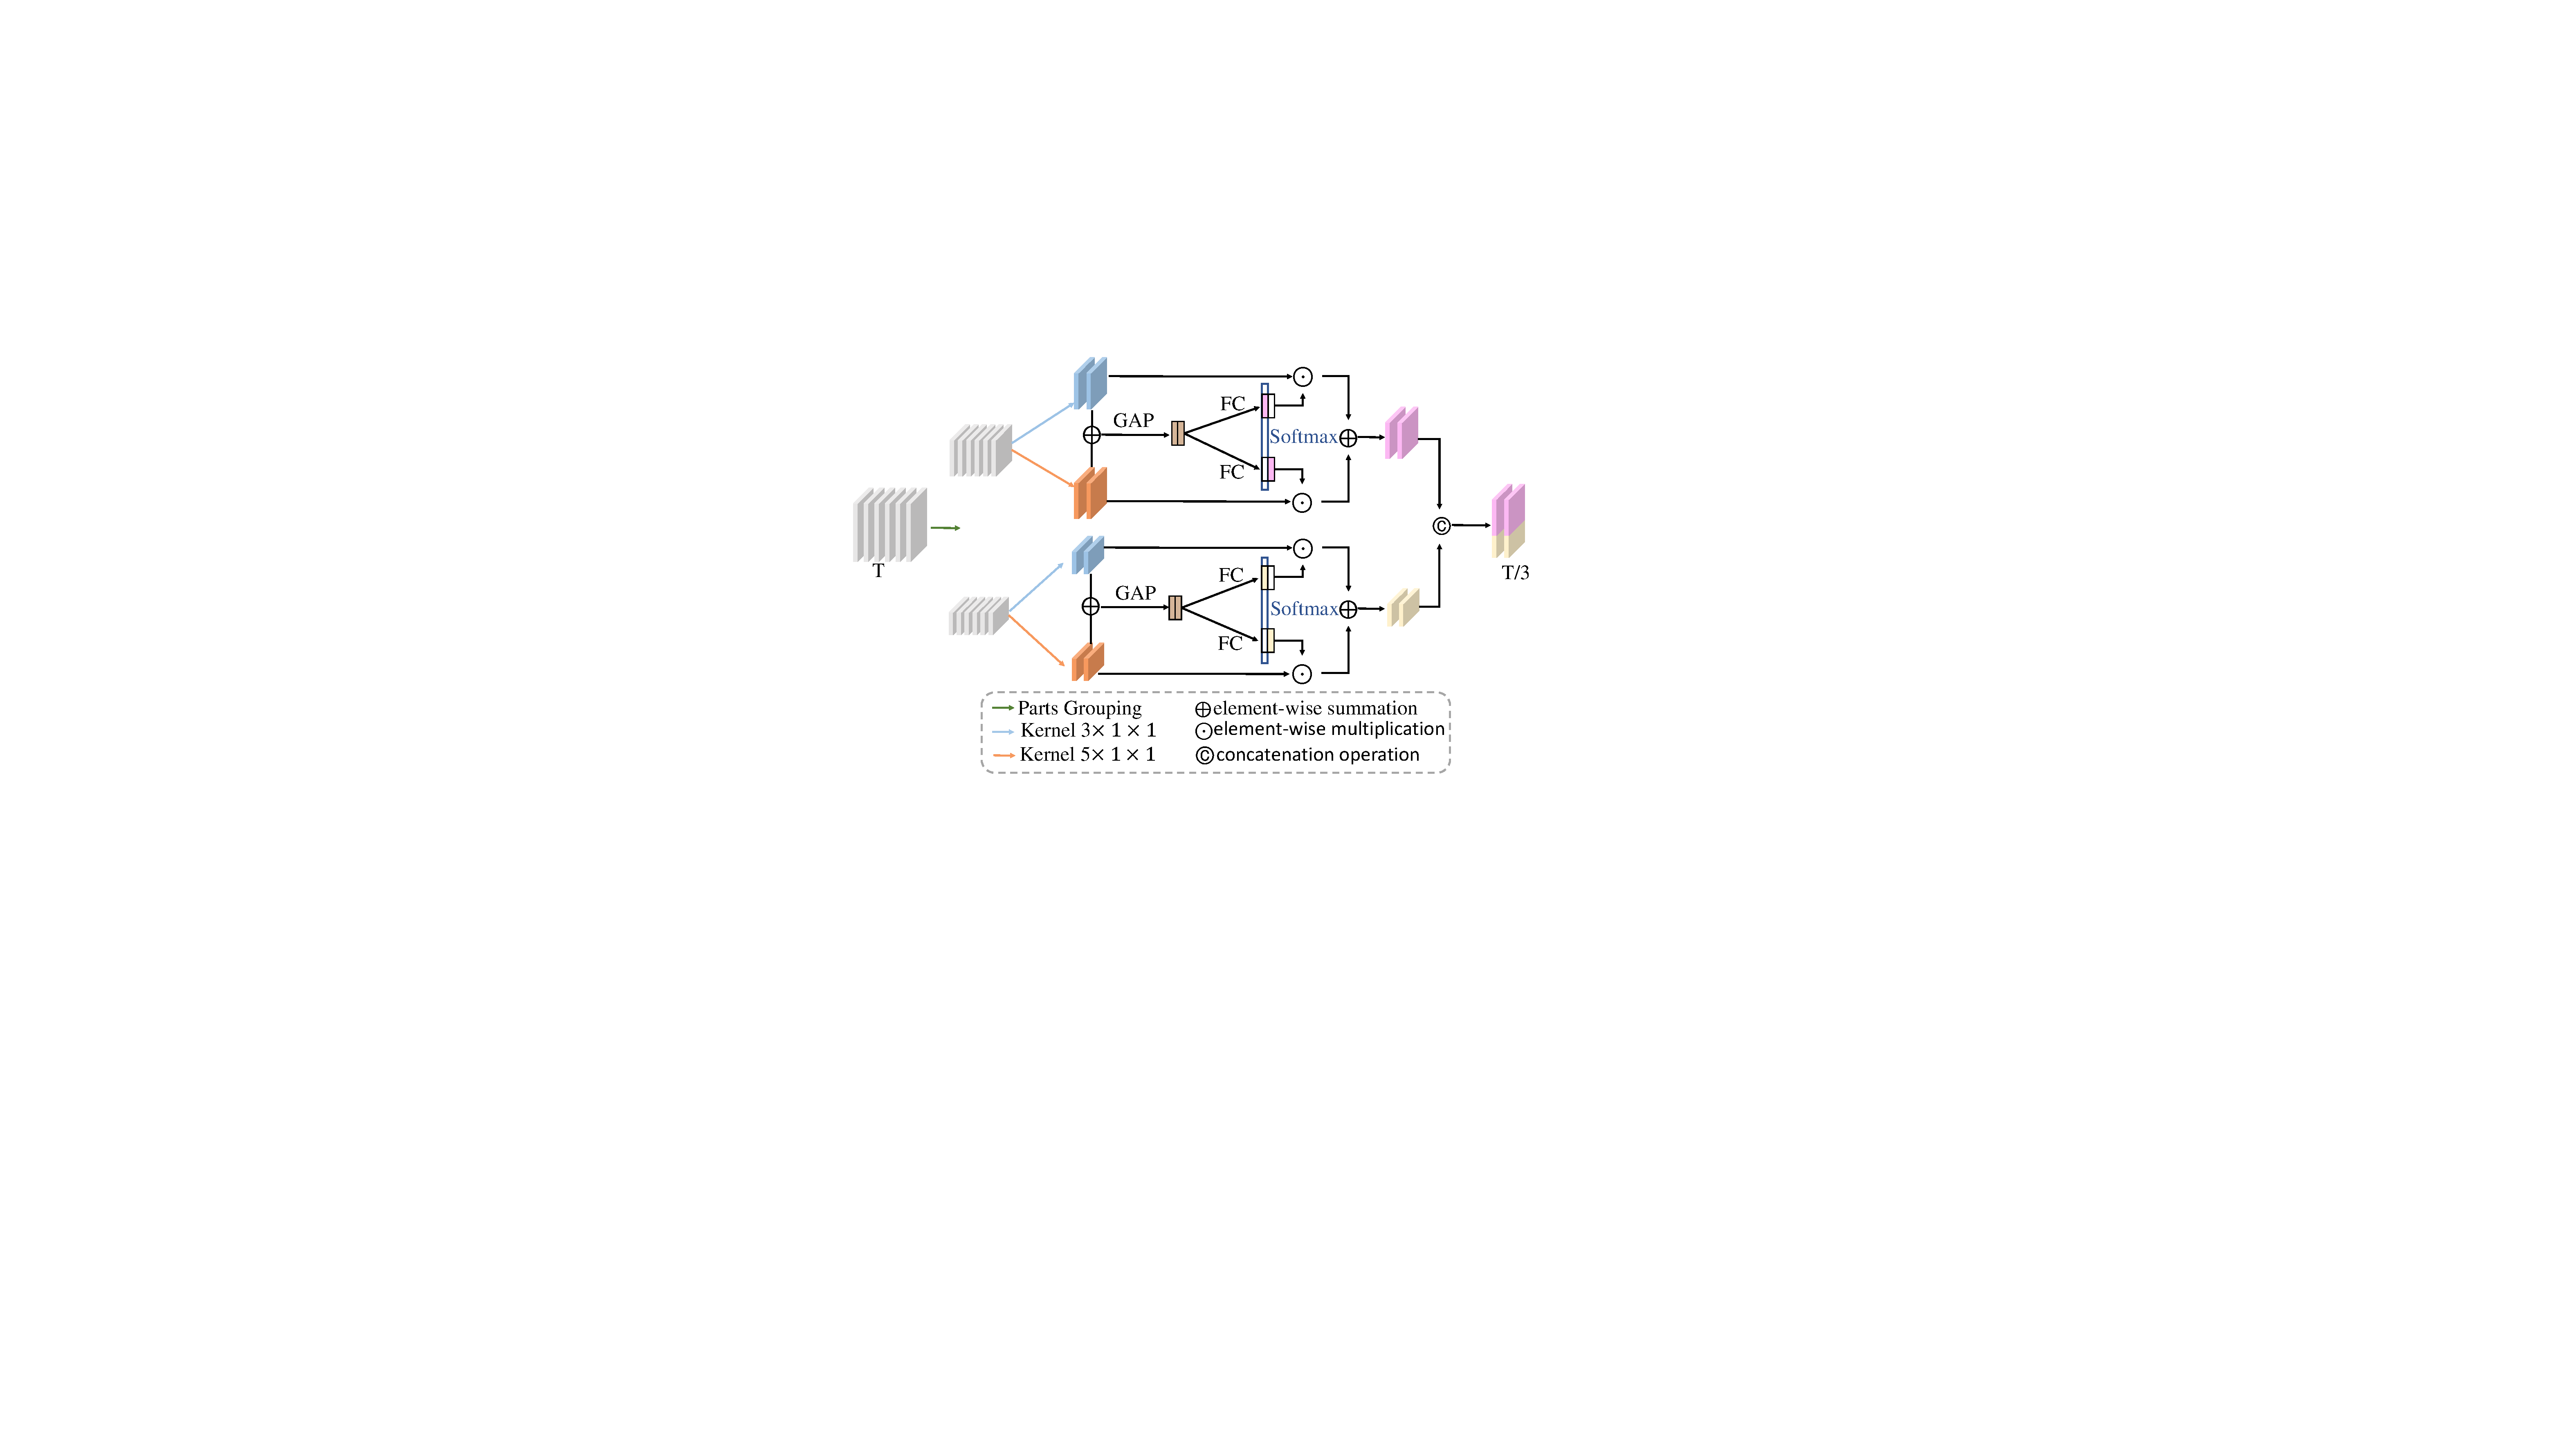
\includegraphics[width=0.8\textwidth]{mma.pdf}
% \caption{FTA}
% }

% \subfloat{1\linewidth}
%      \centering
%   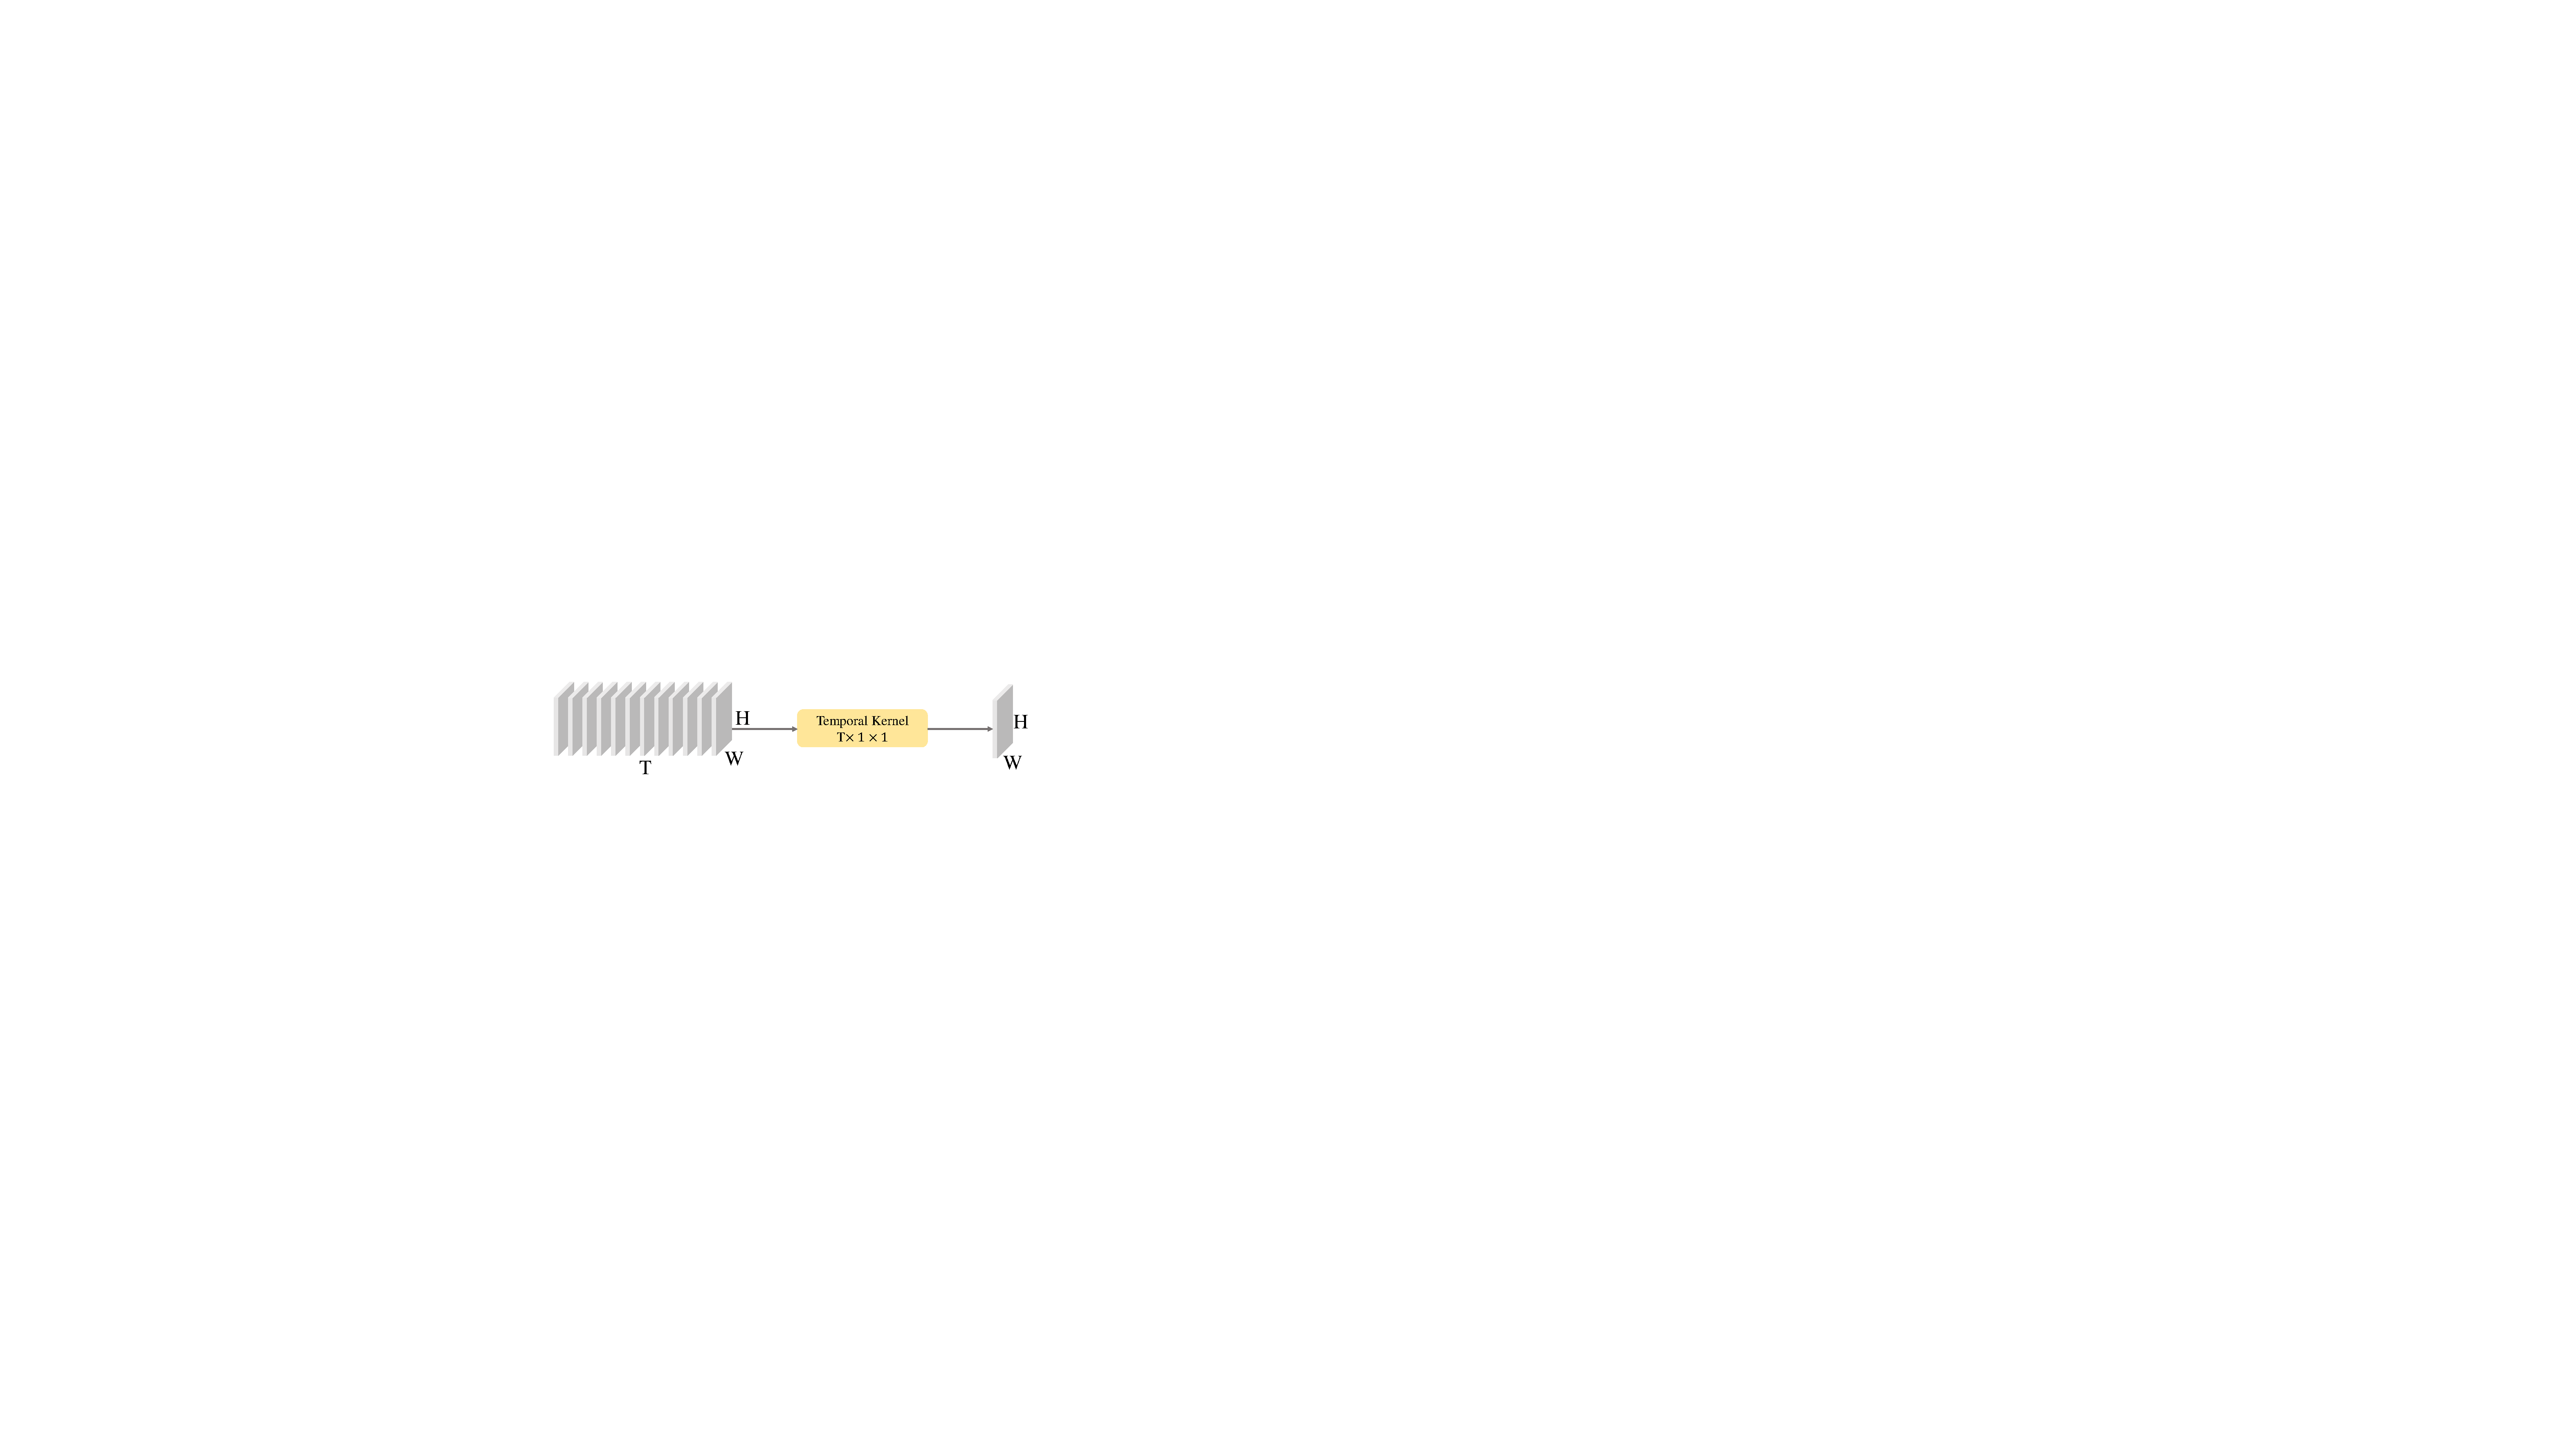
\includegraphics[width=0.8\textwidth]{STA.pdf}
% \caption{STA}
%  \caption{Two temporal aggregation modules. The channel dimension $C$ is omitted for clarity. (a) The detailed structure of the frame-level temporal aggregation (FTA). (b) The detailed structure of the sequence-level temporal aggregation (STA).}
% \label{fig:mma}
% \end{figure}
\begin{figure}[t]%
    \centering
    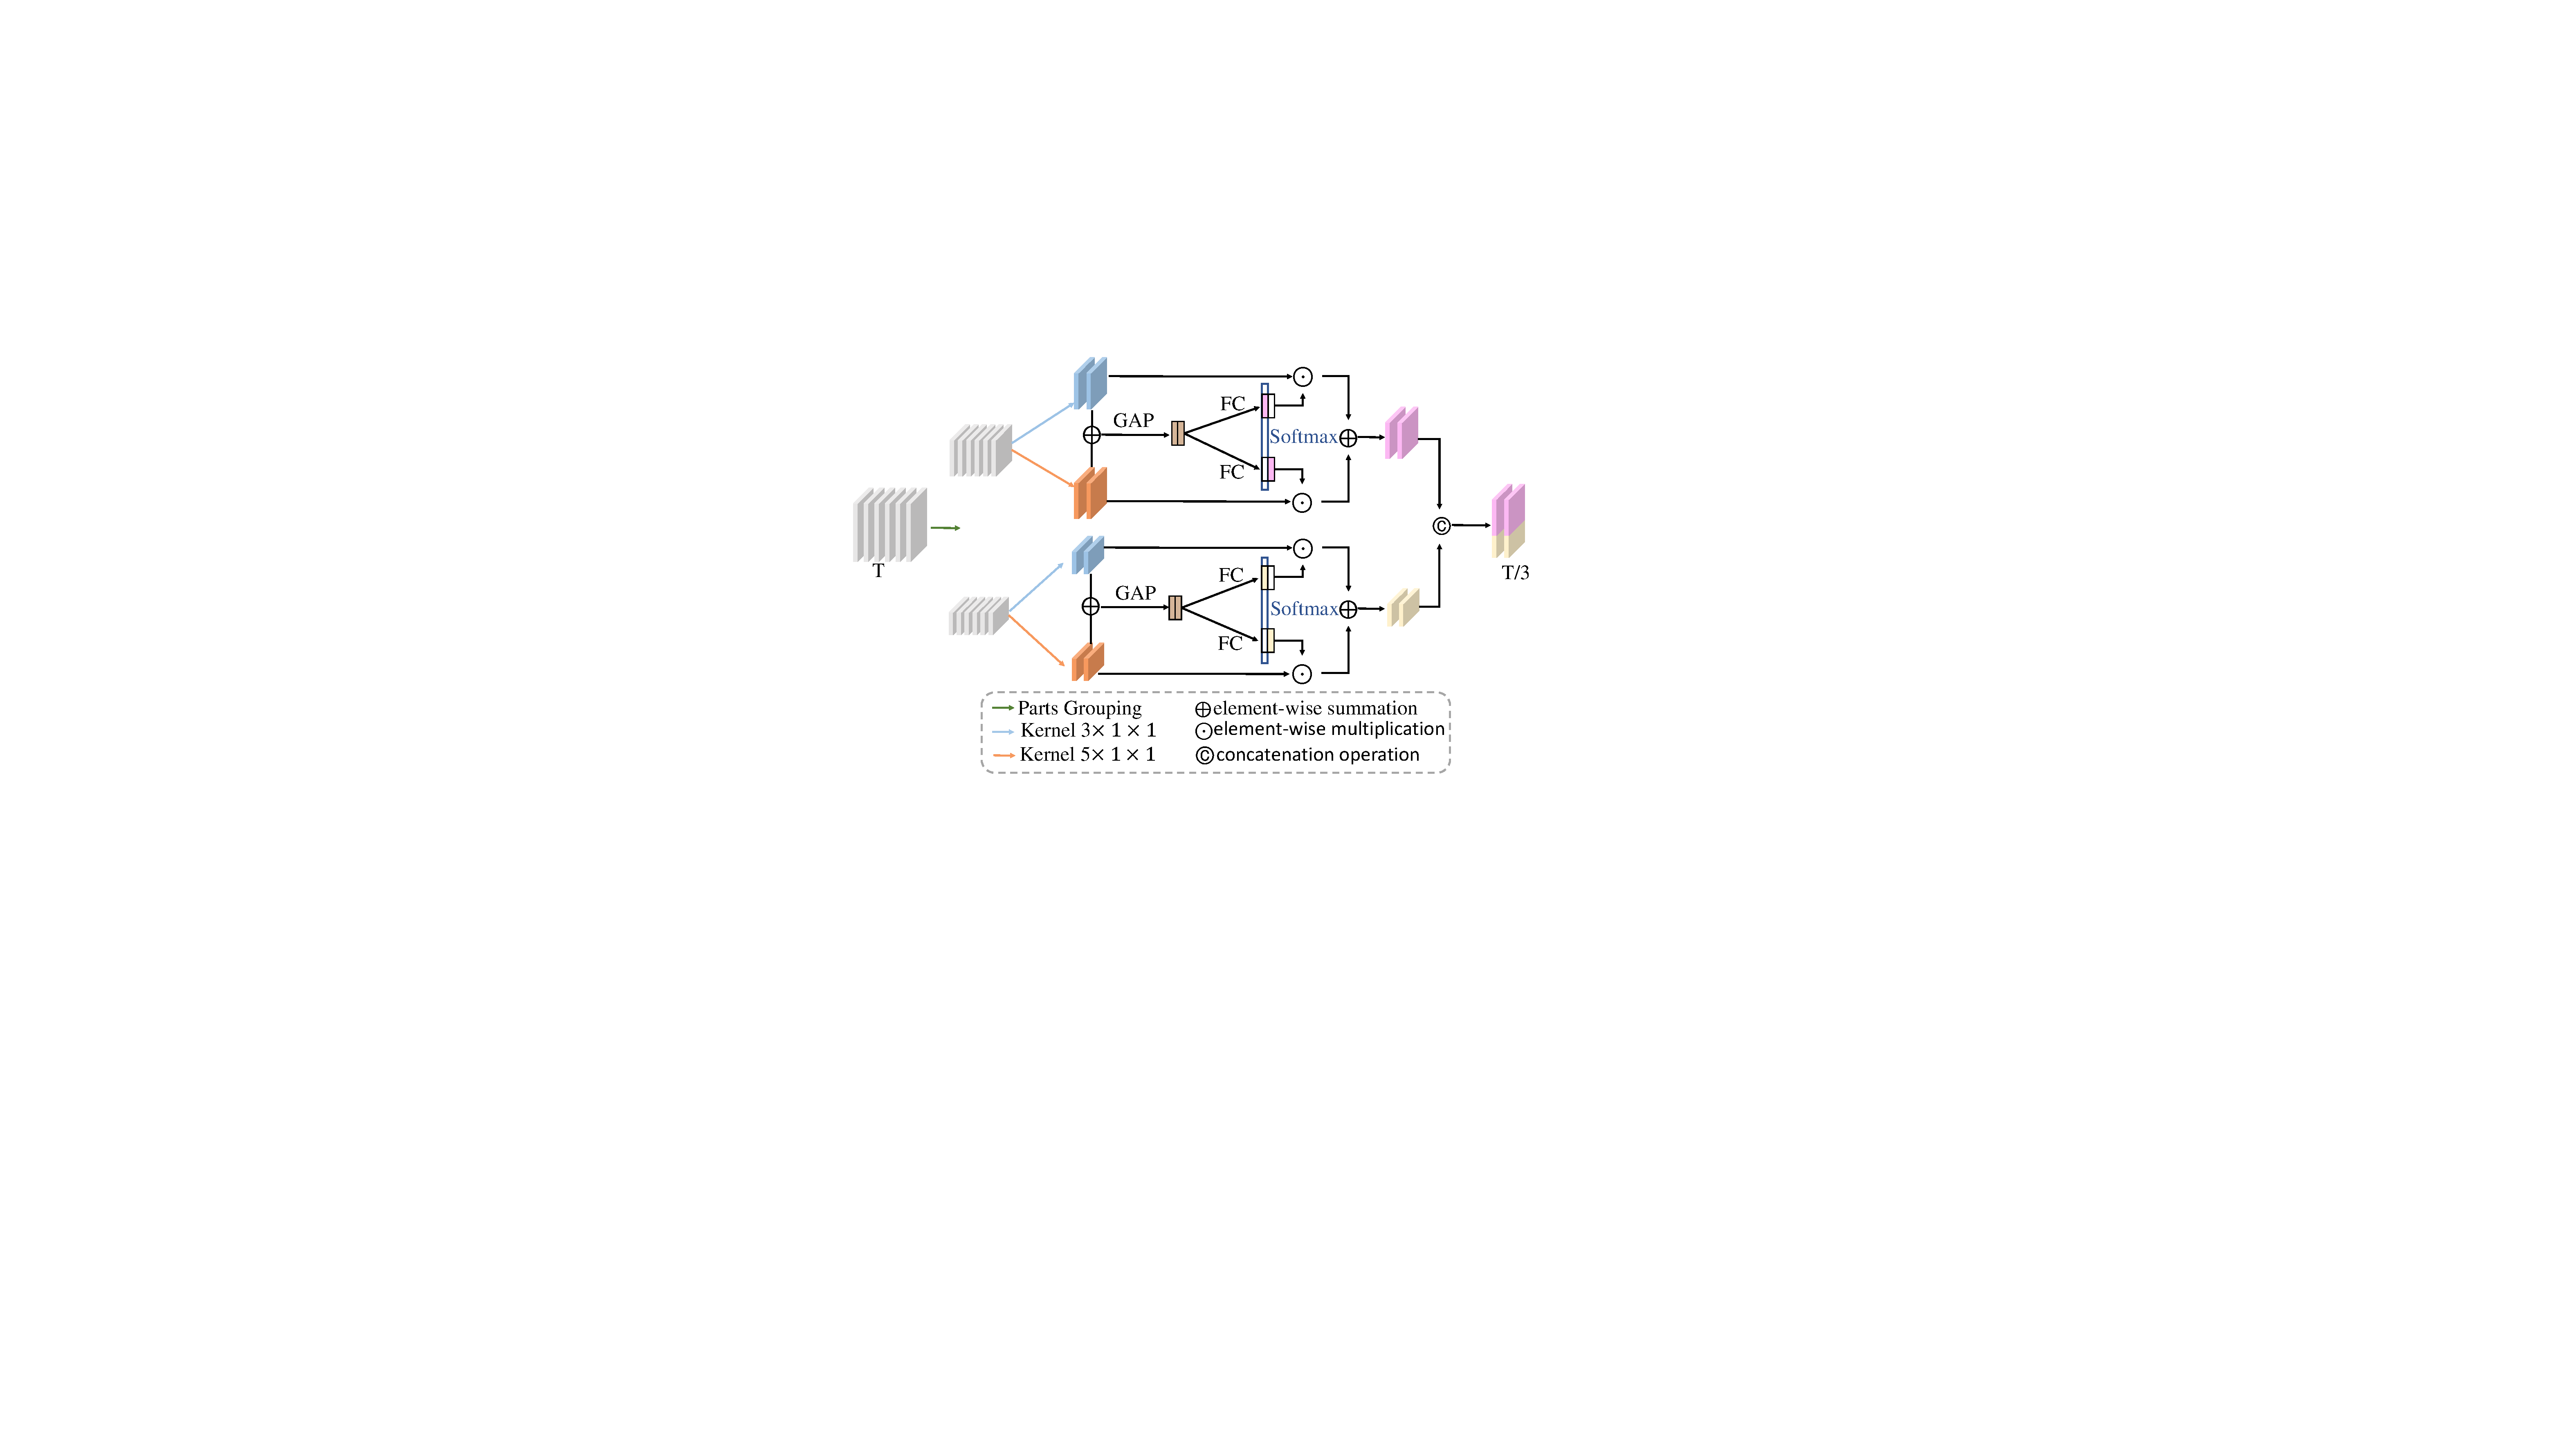
\includegraphics[width=1.0\linewidth]{mma.pdf}
    \caption{The detailed structure of the frame-level temporal aggregation (FTA). For simplicity, we omit the channel dimension $C$.
    }
    \label{fig:mma}
\end{figure}
%The FTA is shown in Fig.~\ref{fig:mma}. Given the hierarchical relation $\mathcal{P}$ introduced in Section \ref{sec:pipe}, FTA first divides the input sequence $X$ into $K_l$ regions based on the partition of the $l$-th level $\mathcal{P}^{(l)}$, resulting in the set of regions $\{X_{j}^{(l)}\}_{j=1}^{K_l}$. Then, we perform $V$ parallel pooling operation on the $j$-th input region feature $X_{j}^{(l)}$ for the $l$-th level of FTA, denoted as:
A gait sequence may contain several redundant frames due to factors such as the acquisition frame rate and pace frequency. To reduce computational costs, some methods compress a gait sequence by aggregating its local clips \cite{lin2021gait,lin2021gaitmask}. In the proposed frame-level temporal aggregation (FTA) strategy, we consider both the gait structure and the multiscale temporal information. Given the $j$-th gait region at the $l$-th level, $X_{j}^{(l)}$, we first fuse the features of the two temporal scales using the following formula:
\begin{equation}
\begin{aligned}
\hat{U}_{j}^{(l)}&=U_{j,1}^{(l)}+U_{j,2}^{(l)}\\ &=\text{Max}_{3 \times 1 \times 1}^{3\times 1 \times 1}\left(X_{j}^{(l)}\right)
    +\text{Max}_{5 \times 1 \times 1}^{3\times 1 \times 1}\left(X_{j}^{(l)}\right),
\end{aligned}
    % \hat{U}_{j}^{(l)}=U_{j,1}^{(l)}=\sum_{v=1}^{V}\psi_{v}\left(X_{j}^{(l)}\right),v\in \left\{1,2,\cdots,V\right\},
    \label{equ:poolfeature}
\end{equation}
where $\text{Max}_{3 \times 1 \times 1}^{3\times 1 \times 1}\left(\cdot\right)$ and $\text{Max}_{5 \times 1 \times 1}^{3\times 1 \times 1}\left(\cdot\right)$ denote max pooling operations with kernel sizes of $3\times 1 \times 1$ and $5\times 1 \times 1$ respectively, both with stride of $3 \times 1 \times 1$. $\hat{U}_{j}^{(l)}$, $U_{j,1}^{(l)}$ and  $U_{j,2}^{(l)}$ have the same size of $(C,\frac{T}{3},H_j^{(l)},W)$.
The output of Eq.(\ref{equ:poolfeature}), $\hat{U}_{j}^{(l)}$, is the element-wise summation of the aggregation results of the two scales, $U_{j,1}^{(l)}$ and $U_{j,2}^{(l)}$, which reduces the temporal dimension of the input from  $T$ to $\frac{T}{3}$.

Then, the FTA model produces frame-level weights, which can be expressed as:
% \begin{equation}
%     \begin{gathered}
%         Z_{j,1}^{(l)}=\text{FC}_{j,1}^{(l)}\left(\text{GAP}\left(\hat{U}_j^{(l)}\right)\right),\\
%         Z_{j,2}^{(l)}=\text{FC}_{j,2}^{(l)}\left(\text{GAP}\left(\hat{U}_j^{(l)}\right)\right),\\
%         \mathcal{W}_{j,1,c}^{(l)}=\frac{e^{Z_{j,1,c}^{(l)}}}{e^{Z_{j,1,c}^{(l)}}+e^{Z_{j,2,c}^{(l)}}},\mathcal{W}_{j,2,c}^{(l)}=\frac{e^{Z_{j,2,c}^{(l)}}}{e^{Z_{j,1,c}^{(l)}}+e^{Z_{j,2,c}^{(l)}}},
%     \end{gathered}
%         % \hat{U}_j^{(l)}&=g\left(\sum_{n=1}^N U_{j,n}^{(l)}\right)\\
%         \label{equ:weight}
% \end{equation}
\begin{equation}
    \begin{gathered}
        Z_{j,1}^{(l)}=\text{FC}_{j,1}^{(l)}\left(\text{GAP}\left(\hat{U}_j^{(l)}\right)\right),\\
        Z_{j,2}^{(l)}=\text{FC}_{j,2}^{(l)}\left(\text{GAP}\left(\hat{U}_j^{(l)}\right)\right),
    \end{gathered}
        % \hat{U}_j^{(l)}&=g\left(\sum_{n=1}^N U_{j,n}^{(l)}\right)\\
        \label{equ:weight}
\end{equation}
where $\text{GAP}\left(\cdot\right)$ represents the global mean pooling along spatial dimension.
$\text{FC}_{j,1}\left(\cdot\right)$ and $\text{FC}_{j,2}\left(\cdot\right)$ are two independent fully connected layers that generate the frame selection weighting tensors, $Z_{j,1}^{(l)}$ and $ Z_{j,2}^{(l)} \in \mathbb{R}^{C  \times \frac{T}{3} \times 1 \times 1}$, for $U_{j,1}^{(l)}$ and $U_{j,2}^{(l)}$, respectively. The weights are further normalized across the two scales, which can be written as follows:
\begin{equation}
  \label{equ:normalize}
       \mathcal{W}_{j,s,c,t}^{(l)}=\frac{e^{Z_{j,s,c,t}^{(l)}}}{e^{Z_{j,1,c,t}^{(l)}}+e^{Z_{j,2,c,t}^{(l)}}}   \quad s\in \{1,2\},
 \end{equation}
where $\mathcal{W}_{j,s,c,t}^{(l)} \in \mathbb{R}^{1 \times 1 \times 1 \times 1}$ is the weight value of the $c$-th channel of the $t$-th frame.
       %,w_{j,2,c,t}^{(l)}=\frac{e^{z_{j,2,c,t}^{(l)}}}{e^{z_{j,1,c,t}^{(l)}}+e^{z_{j,2,c,t}^{(l)}}},
Combining Eq.~(\ref{equ:poolfeature}) and Eq.~(\ref{equ:normalize}), the $j$-th output region feature $Y_{\Omega,j}^{(l)} \in \mathbb{R}^{C^{(l)} \times \frac{T}{3} \times H_j^{(l)} \times W}$ for the $l$-th level of FTA can be obtained as follows:
\begin{equation}
    % Y_{\Omega,j}^{(l)}=\sum_{v=1}^{V}\left(\mathcal{W}_{j,v}^{(l)} \odot U_{j,n}^{(l)}\right)
    Y_{\Omega,j}^{(l)}=\mathcal{W}_{j,1}^{(l)}\odot U_{j,1}^{(l)}+\mathcal{W}_{j,2}^{(l)}\odot U_{j,2}^{(l)},
\end{equation}
where $\mathcal{W}_{j,1}^{(l)}, \mathcal{W}_{j,2}^{(l)} \in \mathbb{R}^{C \times \frac{T}{3} \times 1 \times 1}$ are two weight tensors calculated using Eq.~(\ref{equ:poolfeature}), and $\odot$ represents element-wise multiplication operation. The FTA module outputs $Y^{(l)}_{\Omega}\in \mathbb{R}^{C \times \frac{T}{3} \times H \times W}$ by concatenating the $K_l$ gait regions of level $l$, where $Y^{(l)}_{\Omega}=\left[Y_{\Omega,1}^{(l)},Y_{\Omega,2}^{(l)},\ldots,Y_{\Omega,K_l}^{(l)}\right]$.





%The final output of FTA, $Y^{(l)}_{\Omega}$, is a concatenation of all outputs of the weighted sum operation, and it has a shape of $C \times \frac{T}{3} \times H \times W$.



%$Y^{(l)}_{\Omega}=\left[Y_{\Omega,1}^{(l)},Y_{\Omega,2}^{(l)},\ldots,Y_{\Omega,K_l}^{(l)}\right]$,


%where $\mathcal{W}_{j,1,c}^{(l)} \in \mathbb{R}^{1 \times \frac{T}{3} \times 1 \times 1}$  is the $c$-th  normalized channel value  of the weight tensors for the two scales, denoted as $\mathcal{W}_{j,1}^{(l)}$ and $\mathcal{W}_{j,2}^{(l)} \in \mathbb{R}^{C \times \frac{T}{3} \times 1 \times 1}$.





%where $\odot$ denotes element-wise multiplication operation.


%Finally, all outputs of the weighted sum operation are concatenated, which can be written as $Y^{(l)}_{\Omega}=\left[Y_{\Omega,1}^{(l)},Y_{\Omega,2}^{(l)},\ldots,Y_{\Omega,K_l}^{(l)}\right]$, $Y^{(l)}_{\Omega} \in \mathbb{R}^{C  \times \frac{T}{3} \times H \times W}$ is the output of FTA.

% Finally, concatenate all outputs of weighted sum operation, wich can be written as $Y^{(l)}_{\Omega}=\left[Y_{\Omega,1}^{(l)},Y_{\Omega,2}^{(l)},\ldots,Y_{\Omega,K_l}^{(l)}\right]$, $Y^{(l)}_{\Omega} \in \mathbb{R}^{C  \times \frac{T}{3} \times H \times W}$ is the output of FTA.
% each $Y_{fta,j}^{(l)}$ is concated on height, we can obtain $Y^{(l)}=\left[Y_{fta,j}^{(l)}\right]$, where $Y^{(l)}_{\Omega} \in \mathbb{R}^{C^{(l)}  \times \frac{T}{3} \times H \times W}$ is the output of FTA.

% Then the $j$-th output region feature for the $l$-th level of FTA, $X_{fta,j}^{(l)}$, can be defined as follows:
% \begin{equation}
%     Y_{fta,j}^{(l)}=g\left(\sum_{n=1}^{N}\psi_{n}\left(X_{i,j}^{(l)}\right)\right),
% \end{equation}

% % n\in \left\{1,2,\cdots,N\right\},

% Given the hierarchical relation $\mathcal{P}$ introduced in Section \ref{sec:pipe}, FTA first divides the output feature map $Y^{(l)}$ into $K_l$ regions based on the partition of the $l$-th level $\mathcal{P}^{(l)}$, resulting in the set of regions $\{Y_{j}^{(l)}\}_{j=1}^{K_l}$. Then the $l$-th level of FTA, $\Omega^{(l)}$, can be represented as:
% \begin{equation}
%  \begin{aligned}
%         Y_{fta}^{(l)}=\Omega^{(l)}\left(X^{(l)}\right)=\left[{f_{mtp,1}\left(X_1^{(l)}\right),}\right.&\\
%         \left.{f_{mtp,2}\left(X_2^{(l)}\right),\ldots, f_{mtp,K_l}\left(X_{K_l}^{(l)}\right)}\right]
%     \end{aligned}
% \end{equation}
% where $f_{mtp,j}\left(\cdot\right)$ represents the independent MTP operation applied to the $j$-th region. $Y_{fta}^{(l)} \in \mathbb{R}^{C_l \times \frac{T}{3} \times H \times W}$ is the output of FTA. Next, we describe the details of the MTP.
% % \begin{equation}
% %     \begin{aligned}
% %   Y_{fta}^{(l)} =  \biggl[ & Y_i^{M}, \Gamma^{(L-1)}\left(Y_j^{(L-1)}\right),  \ldots , \nonumber \\
% %   & \Gamma^{(l_{\Omega})}\left(Y_i^{(l_{\Omega})}\right), \Gamma^{(2)}\left(Y_i^{(2)}\right), \Gamma^{(1)}\left(Y_i^{(1)}\right) \biggl]
% % \end{aligned}
% % \end{equation}

% % The FTA is shown in Fig.~\ref{fig:mma}. Assume that the output after the $l$-th ARME is $\mathbf{F} \in \mathbb{R}^{C_l \times T \times H \times W}$, first, we split $\mathbf{F}$ into $k$ parts, denoted as $\mathbf{F}_{part}=\left\{\mathbf{F}_i \mid i=1,2,\cdots, k\right\}$, where $\mathbf{F}_i\in\mathbb{R}^{C_l \times T \times \frac{H}{k} \times W}$. According the parts grouping results $I^{(l)}$ in Sec.~\ref{sec:pipe}, grouping $\mathbf{F}_{part}$, we can obtain the features $\mathbf{F}^{(l)}=\left\{\mathbf{F}^{(l)}_g \mid g=1,2,\cdots,G_l\right\}$.  Next, the process of temporal aggregation can be denoted as
% % \begin{equation}
% %     \mathbf{F}_{fta}=\left[f_{mtp,g}\left(\mathbf{F}^{(l)}_g\right)\right]
% % \end{equation}
% % where $f_{mtp,g}\left(\cdot\right)$ represents the MTP operation.  $\mathbf{F}_{fta} \in \mathbb{R}^{C_l \times \frac{T}{3} \times H \times W}$ is the output of FTA. Next, we describe the details of the MTP.
% % Note that the $f_{mtp}\left(\cdot\right)$ used for each $I_{l,g}^{fe}$ is separate.

% Assume that the input of MTP is $U \in \mathbb{R}^{C \times T \times H \times W}$. MTP performs $n$ parallel operations on $U$, the process can be denoted as
% \begin{equation}
%     Z_{i}=\psi_{max,i}\left(U\right),i\in \left\{1,2,\cdots,n\right\},
%     \label{equ:poolfeature}
% \end{equation}
% %其中$Y^{(i) \in \mathbb{R}^{C \times \frac{T}{3} \times H \times W}$是输出特征图，$\textbf{MaxPool3D}^{(i)$由核大小为$2(k-1)+1\times 1 \times 1$,步长为$3\times 1 \times 1$的3D最大池化操作实现。
% where $Z_{i} \in \mathbb{R}^{C \times \frac{T}{3} \times H \times W}$ is the output feature map and $\psi_{max,i}\left(\cdot\right)$ max pooling with kernel of $\left(2i+1\right)\times 1 \times 1$ and stride of $3 \times 1 \times 1$. Next, the element-wise summation is used to fuse $Z_{i}$, and then global average pooling (GAP) is used to compress the spatial dimension of $Z_{i}$. It can be formulated as
% \begin{equation}
%     \hat{Z}=\text{GAP}\left(\sum_{i=1}^{n}Z_{i}\right),
% \end{equation}
% where $\hat{Z}\in \mathbb{R}^{C \times \frac{T}{3} }$ is the output after GAP. Frame-level select weights for different temporal scales are obtained according to $\hat{Z}$, which is achieved through $n$ fully connected layers and a softmax layer. The process can be formulated as:
% \begin{equation}
%     E_{i,c} = \frac{e^{\text{FC}_{i,c}\left(\hat{Z}\right)}}{\sum_{j=1}^{n}e^{\text{FC}_{j,c}\left(\hat{Z}\right)}},i \in \{1,2,\cdots,n\},
%     \label{equ:weight}
% \end{equation}
% where $E_{i} \in \mathbb{R}^{C \times \frac{T}{3}}$ denotes the weight generated for each temporal scale, $c$ is the index of $c$-th channel of $E_{i}$, $\text{FC}_{i}\left(\cdot\right)$ denotes the fully connected layer. Finally, the feature map for soft-attention fusion is obtained by combining Eq.~\ref{equ:weight} and Eq.~\ref{equ:poolfeature}, and denoted as
% \begin{equation}
%     F_{mtp} = \sum_{i=1}^{n}\left(Y_{i} \odot \textrm{Reshape} \left(E_{i} \right)\right),
% \end{equation}
% where $F_{mtp} \in \mathbb{R}^{C \times \frac{T}{3} \times H \times W}$ is the output of MTP, $\textrm{Reshape}\left(\cdot\right)$ reshapes $E^{i} \in \mathbb{R}^{C \times \frac{T}{3}}$ to $E^{i} \in \mathbb{R}^{C \times \frac{T}{3} \times 1 \times 1}$ to match the size of $Y_{i} \in \mathbb{R}^{C \times \frac{T}{3} \times H \times W}$ and $\odot$ denotes element-wise multiplication operation.

% \subsection{Loss Functions}
% \label{sec:loss}

% To obtain sequence-level features, we introduce a Temporal Pooling (TP) \cite{fan2020gaitpart,lin2020gait,lin2021gait,lin2021gaitmask} operation to aggregate the global temporal information. Assume that the feature map $\mathbf{F}_{fe} \in \mathbb{R}^{C \times \frac{T}{3} \times H \times W}$ is the output of feature extractor, which, after the TP operation, can be formulated as:
% \begin{equation}
%     \mathbf{F}_{tp}=\textrm{TP}\left(\textbf{F}_{fe}\right),
% \end{equation}
% %其中$X_{tp} \in \mathbb{R}^{C \times \times H \times W}$是TP操作的输出。
% where $\mathbf{F}_{tp} \in \mathbb{R}^{C \times H \times W}$ is the output feature of the TP operation.

% Then we introduce a Generalized Mean pooling (GeM) \cite{lin2021gait,lin2021gaitmask} operation to adaptively aggregate the spatial features of $\mathbf{F}_{tp}$. Moreover, a separable fully connected layer and a Batchnorm layer are used to map the features to the discriminative space further. The process can be formulated as:
% \begin{equation}
%     \mathcal{G} = \textrm{BN}\left( \textrm{SeFC}\left(\text{GeM}\left(\mathbf{F}_{tp}\right)\right)\right),
% \end{equation}
% %其中$Y \in \mathbb{R}^{C \times s}$是空间特征映射的输出，$\mathbf{SeFC}\left(\cdot\right)$是独立的全连接层，$\textbf{GeMP}\left(\right)$是广义平均池化操作。
% where $\mathcal{G} \in \mathbb{R}^{C \times H_2}$ is the output of the spatial feature mapping, $H_2$ represents the number of horizontal bins, $\textrm{SeFC}\left(\cdot\right)$ is the separable fully connected layer and $\textrm{BN}\left(\cdot\right)$ represents the BatchNorm layer.

% Finally, the feature $\mathcal{G}$ is trained using triplet loss $\mathcal{L}_{tri}$, and the feature $\mathcal{A} \in \mathbb{R}^{C_2 \times H_2}$ obtained from the feature $\mathcal{G}$ through a separable fully connected layer are trained using cross-entropy loss $\mathcal{L}_{ce}$. The $C_2$ denotes the number of training categories of subjects. The total loss $\mathcal{L}$ can be formulated as:
% \begin{equation}
%     \mathcal{L}=\mathcal{L}_{tri} + \mathcal{L}_{ce}.
% \end{equation}

\begin{table*}[tbp]
  \centering
  \setlength{\abovecaptionskip}{0cm}  %段前
\setlength{\belowcaptionskip}{-0.2cm} %段后
  \caption{Rank-1 accuracy (\%) on CASIA-B under all views and different conditions, excluding identical-view cases. Std denotes the performance sample standard deviation across 11 views.}
  \resizebox{0.95\linewidth}{!}{
    \begin{tabular}{c|c|ccccccccccc|c|c}
    \toprule
    \multicolumn{2}{c|}{Gallery NM \#1-4} & \multicolumn{11}{c|}{$0^{\circ}-180^{\circ}$}                                                         & \multirow{1}[4]{*}{Mean} & \multirow{1}[4]{*}{Std}\\
\cline{1-13}    \multicolumn{2}{c|}{Probe} & $0^{\circ}$    & $18^{\circ}$   & $36^{\circ}$   & $54^{\circ}$   & $72^{\circ}$   & $90^{\circ}$   & $108^{\circ}$  & $126^{\circ}$  & $144^{\circ}$  & $162^{\circ}$  & $180^{\circ}$  &  \\
    \hline
    \multirow{5}[10]{*}{NM \#5-6} & GaitSet \cite{chao2019gaitset} & 90.8  & 97.9  & 99.4  & 96.9  & 93.6  & 91.7  & 95.0    & 97.8  & 98.9  & 96.8  & 85.8  & 95.0 &3.5\\
% \cline{14-14}         & ACL   & 92.0    & 98.5  & \textbf{100.0}   & \textbf{98.9}  & 95.7  & 91.5  & 94.5  & 97.7  & 98.4  & 96.7  & 91.9  & 96.0 \\
          & GaitPart \cite{fan2020gaitpart} & 94.1  & 98.6  & 99.3  & 98.5  & 94.0    & 92.3  & 95.9  & 98.4  & 99.2  & 97.8  & 90.4  & 96.2 &3.1\\
% \cline{14-14}          & MT3D  & 95.7  & 98.2  & 99.0    & 97.5  & 95.1  & 93.9  & 96.1  & 98.6  & 99.2  & 98.2  & 92.0    & 96.7 \\
         & 3D Local \cite{huang20213d} & 96.0    & \underline{99.0}    & \underline{99.5}  & \underline{98.9}  & 97.1  & 94.2  & 96.3  & 99.0    & 98.8  & 98.5  & 95.2  & 97.5&1.8 \\
          & CSTL \cite{huang2021context} & 97.2  & \underline{99.0}    & 99.2  & 98.1  & 96.2  & \underline{95.5}  & \underline{97.7}  & 98.7  & 99.2  & \underline{98.9}  & 96.5  & \underline{97.8} &1.3\\
          & GaitGL \cite{lin2021gait} & 96.0    & 98.3  & 99.0    & 97.9  & 96.9  & 95.4  & 97.0    & 98.9  & \underline{99.3}  & 98.8  & 94.0    & 97.4 &1.7\\
          & LagrangeGait \cite{chai2022lagrange} & 95.7  & 98.1  & 99.1  & 98.3  & 96.4  & 95.2  & 97.5  & 99.0    & \underline{99.3}  & \underline{98.9}  & 94.9  & 97.5 &1.6\\
         & MetaGait \cite{dou2022metagait} & \underline{97.3}  & \textbf{99.2}  & \underline{99.5}  & \textbf{99.1}  & \underline{97.2}  & \underline{95.5}  & 97.6  & \underline{99.1}    & \underline{99.3}  & \textbf{99.1}  & \underline{96.7}  & \textbf{98.1} & \underline{1.3} \\
\cline{2-15}          & \textbf{Ours} & \textbf{97.6}  & 98.0  & \textbf{99.6}    & 98.2    & \textbf{97.4}  & \textbf{96.5}  & \textbf{97.9}  & \textbf{99.3}  & \textbf{99.4}  & 98.4  & \textbf{97.0}  & \textbf{98.1} & \textbf{1.0}\\
    \hline
    \multirow{4}[12]{*}{BG \#1-2} & GaitSet \cite{chao2019gaitset} & 83.8  & 91.2  & 91.8  & 88.8  & 83.3  & 81.0    & 84.1  & 90.0    & 92.2  & 94.4  & 79.0    & 87.2 &4.9 \\
           & GaitPart \cite{fan2020gaitpart} & 89.1  & 94.8  & 96.7  & 95.1  & 88.3  & 84.9  & 89.0    & 93.5  & 96.1  & 93.8  & 85.8  & 91.5&4.2 \\
% \cline{14-14}           & MT3D  & 91.0    & 85.4  & 97.5  & 94.2  & 92.3  & 86.9  & 91.2  & 95.6  & 97.3  & 96.4  & 86.6  & 93.0 \\
          & 3D Local \cite{huang20213d} & 92.9  & 95.9  & \textbf{97.8}  & 96.2  & 93.0    & 87.8  & 92.7  & 96.3  & 97.9  & 98.0    & 88.5  & 94.3&3.5 \\
           & CSTL \cite{huang2021context}  & 91.7  & 96.5  & 97.0    & 95.4  & 90.9  & 88.0    & 91.5  & 95.8  & 97.0    & 95.5  & 90.3  & 93.6 &3.0\\
           & GaitGL \cite{lin2021gait} & 92.6  & \underline{96.6}  & 96.8  & 95.5  & 93.5  & 89.3  & 92.2  & 96.5  & 98.2  & 96.9  & 91.5  & 94.5&2.8 \\
          & LagrangeGait \cite{chai2022lagrange} & \underline{94.2}  & 96.2  & \underline{96.8}  & 95.8  & 94.3  & 89.5  & 91.7  & 96.8  & 98.0    & 97.0    & 90.9  & 94.6&2.7 \\
          & MetaGait \cite{dou2022metagait} & 92.9  & \textbf{96.7}  & 97.1  & \underline{96.4}  & \underline{94.7}  & \underline{90.4}  & \underline{92.9}  & \textbf{97.2}  & \underline{98.5}    & \textbf{98.1}    & \underline{92.3}  & \underline{95.2} &\underline{2.6}\\
\cline{2-15}          & \textbf{Ours} & \textbf{95.0}  & 96.5  & \underline{97.3}  & \textbf{96.6}  & \textbf{95.3}  & \textbf{93.3}  & \textbf{94.6}  & \underline{96.8}  & \textbf{98.6}  & \underline{97.7}  & \textbf{92.9}    & \textbf{95.9}&\textbf{1.7} \\
    \hline
    \multirow{4}[12]{*}{CL \#1-2} & GaitSet \cite{chao2019gaitset} & 61.4  & 75.4  & 80.7  & 77.3  & 72.1  & 70.1  & 71.5  & 73.5  & 73.5  & 68.4  & 50.0    & 70.4&8.0 \\
         & GaitPart \cite{fan2020gaitpart} & 70.7  & 85.5  & 86.9  & 83.3  & 77.1  & 72.5  & 76.9  & 82.2  & 83.8  & 80.2  & 66.5  & 78.7 &6.6\\
% \cline{14-14}          & MT3D  & 76.0    & 87.6  & 89.8  & 85.0    & 81.2  & 75.7  & 81.0    & 84.5  & 85.4  & 82.2  & 68.1  & 81.5 \\
          & 3D Local \cite{huang20213d} & 78.2  & 90.2  & 92.0    & 87.1  & 83.0    & 76.8  & 83.1  & 86.6  & 86.8  & 84.1  & 70.9  & 83.7 &6.2\\
          & CSTL \cite{huang2021context}  & 78.1  & 89.4  & 91.6  & 86.6  & 82.1  & 79.9  & 81.8  & 86.3  & 88.7  & 86.6  & 75.3  & 84.2 &\underline{4.9}\\
          & GaitGL \cite{lin2021gait} & 76.6  & 90.0    & 90.3  & 87.1  & 84.5  & 79.0    & 84.1  & 87.0    & 87.3  & 84.4  & 69.5  & 83.6&6.3 \\
          & LagrangeGait \cite{chai2022lagrange} & 77.4  & 90.6  & \underline{93.2}  & \underline{90.2}  & 84.7  & 80.3  & \underline{85.2}  & 87.7  & 89.3  & 86.6  & 71.0    & 85.1 &6.3\\
          & MetaGait \cite{dou2022metagait} & \underline{80.0}  & \underline{91.8}  & 93.0  & 87.8  & \underline{86.5}  & \underline{82.9}  & \underline{85.2}  & \underline{90.0}  & \underline{90.8}  & \underline{89.3}  & \underline{78.4}    & \underline{86.9} &\textbf{4.6}\\
\cline{2-15}          & \textbf{Ours} & \textbf{82.4}  & \textbf{94.2}  & \textbf{95.0}  & \textbf{91.7}  & \textbf{88.2}  & \textbf{83.3}  & \textbf{88.0}  & \textbf{92.3}  & \textbf{93.1}  & \textbf{91.0}  & \textbf{78.5}  & \textbf{88.9} &5.1\\
    \bottomrule
    \end{tabular}%
    }
  \label{tab:sota-cb}%
\end{table*}%
\section{Experiments}
\label{sec:exper}
\subsection{Datasets and Evaluation Protocols}
\label{sec:dataset}
\noindent\textbf{CASIA-B.} The CASIA-B \cite{yu2006framework} dataset is a widely used benchmark for gait recognition. It contains video sequences of 124 subjects with 11 different views and three walking conditions (normal walking (NM), walking with a bag (BG), and walking with a coat (CL)). Our study follows the protocol outlined in previous works \cite{chao2019gaitset,fan2020gaitpart,lin2021gait,lin2021gaitmask,huang2021context,huang20213d}. The first 74 subjects are used for training, and the remaining 50 subjects are used for testing. During testing, the first four sequences under NM (NM\#01-04) are regarded as the gallery set, and the rest  (NM\#05-06, BG\#01-02, CL\#01-02) are regarded as the probe set.

\noindent\textbf{OUMVLP.} The OUMVLP \cite{NorikoTakemura2018MultiviewLP} is one of the largest gait datasets, containing silhouette sequences of 10,307 subjects. Each subject has a single normal walking condition (NM) with 14 views. According to the protocol provided by the dataset, the first 5,153 subjects are used for training while the remaining 5,154 subjects are used for testing. During the testing phase, the sequences of NM\#01 are assigned to the gallery set, and the sequences of NM\#02 are considered as the probe set.

\noindent\textbf{GREW.} GREW \cite{zhu2021gait} is the first large-scale dataset for gait recognition in the wild, consisting of 128,671 sequences from 26,345 individuals captured by 882 cameras. It includes four data types: four data types: silhouettes, optical flow, 2D pose, and 3D pose. The dataset is divided into a training set with 20,000 subjects and 102,887 sequences, and a testing set with 6,000 subjects and 24,000 sequences. In the testing phase, each subject has two sequences for the gallery set and two for the probe set. The GREW dataset also includes a distractor set, which contains 233,857 unlabeled sequences.


\noindent\textbf{Gait3D.} The Gait3D dataset \cite{zheng2022gait} is a newly proposed dataset for gait recognition in uncontrolled indoor environments, particularly in large supermarkets. It contains 25,309 sequences of 4,000 subjects extracted from 39 cameras, with 18,940 sequences from 3,000 subjects for training and 6,369 sequences from 1,000 subjects for testing. The dataset mainly includes four data types: silhouettes, 2D pose, 3D pose, and 3D mesh. During testing, one sequence per subject is used as the probe set, while the remaining sequences are used as the gallery set.  To evaluate the model's performance, we use accuracy as well as mean average precision (mAP) and mean inverse negative penalty (mINP) \cite{ye2021deep}, which consider multiple instances and hard sample recall.



%The Gait3D \cite{zheng2022gait} dataset is a newly proposed dataset for gait recognition in uncontrolled environments, particularly in large supermarkets. It contains 4,000 subjects and 25,309 sequences extracted from 39 cameras, with 3,000 subjects and 18,940 sequences for training and 1,000 subjects and 6,369 sequences for testing. It also contain four data types: silhouettes, 2D pose, 3D pose, and 3D mesh. During the testing phase, one sequence from each subject is used as the probe set, while the rest of the sequences are used as the gallery set.  In addition to accuracy, we evaluate the model using mean average precision (mAP) and mean inverse negative penalty (mINP) \cite{ye2021deep}, which consider multiple instances and hard sample recall.

% \begin{table}[htbp]
%   \centering
%   \caption{The detailed architecture of the proposed HSTL on CASIA-B. The In\_C and Out\_C represent the input channel and output channel of each layer respectively, and the Kernel means the size of the convolution kernel or pooling kernel. We index each body part 0 to 7 in spatial order from top to bottom.}
%   \resizebox{\linewidth}{!}{
%     \begin{tabular}{c|c|c|c|c|c|c}
%     \toprule
%     Block & Layer & In\_C & Out\_C & Kernel & G     & Parts grouping \\
%     \hline
%     ARME  & Conv3d & 1     & 32    & (3,3,3) & 1     & $-$ \\
%     \hline
%     \multirow{2}[1]{*}{ARME} & Conv3d & 32    & 32    & (3,3,3) & 2     & $[0,1,2,3,4]$,$[5,6,7]$ \\
% \cline{2-7}          & Conv3d & 32    & 64    & (3,3,3) & 2     & $[0,1,2,3,4]$,$[5,6,7]$ \\
%     \hline
%     FTA   & MaxPool & 64    & 64    & (3,1,1),(5,1,1) & $-$     & $-$ \\
%     \hline
%     \multirow{2}[1]{*}{ARME} & Conv3d & 64    & 128   & (3,3,3) & 4     & $[0]$,$[1,2,3,4]$,$[5,6]$,$[7]$ \\
% \cline{2-7}          & Conv3d & 128   & 128   & (3,3,3) & 4     & $[0]$,$[1,2,3,4]$,$[5,6]$,$[7]$ \\
%     \bottomrule
%     \end{tabular}%
%     }
%   \label{tab:pcb-str}%
% \end{table}%


% Table generated by Excel2LaTeX from sheet 'Sheet1'
% \begin{table}[htbp]
%   \centering
%   \setlength{\abovecaptionskip}{0cm}  %段前
% \setlength{\belowcaptionskip}{-0.2cm} %段后
%   \caption{The detailed architecture of the proposed HSTL on CASIA-B. The In\_C and Out\_C represent the input channel and output channel of each layer respectively, and the Kernel means the size of the convolution kernel or pooling kernel. We index each body part 1 to 8 in spatial order from top to bottom.}
%   % \setlength{\tabcolsep}{0.5mm}{
%    \resizebox{\linewidth}{!}{
%   \small
%     \begin{tabular}{c|c|c|c|c|c|c}
%     \toprule
%     Block & Layer & In\_C & Out\_C & Kernel & G     & Parts grouping \\
%     \hline
%     ARME  & Conv3d & 1     & 32    & (3,3,3) & 1     & $\{[1,2,3,4,5,6,7,8]\}$ \\
%     \hline
%     \multirow{2}[1]{*}{ARME} & Conv3d & 32    & 32    & (3,3,3) & 2     & $\{[1,2,3,4,5]$,$[6,7,8]\}$ \\
% \cline{2-7}          & Conv3d & 32    & 64    & (3,3,3) & 2     & $\{[1,2,3,4,5]$,$[6,7,8]\}$ \\
%     \hline
%     \multirow{2}[1]{*}{FTA} & \multirow{2}[1]{*}{MaxPool} & \multirow{2}[1]{*}{64} & \multirow{2}[1]{*}{64} & (3,1,1) & \multirow{2}[1]{*}{-} & \multirow{2}[1]{*}{-} \\
%           &       &       &       & (5,1,1) &       &  \\
%     \hline
%     \multirow{2}[1]{*}{ARME} & Conv3d & 64    & 128   & (3,3,3) & 4     & $\{[1]$,$[2,3,4,5]$,$[6,7]$,$[8]\}$ \\
% \cline{2-7}          & Conv3d & 128   & 128   & (3,3,3) & 4     & $\{[1]$,$[2,3,4,5]$,$[6,7]$,$[8]\}$ \\
%     \bottomrule
%     \end{tabular}%
%     }
%   \label{tab:pcb-str}%
% \end{table}%

% Table generated by Excel2LaTeX from sheet 'Sheet1'
% \begin{table}[htbp]
%   \centering
%     \setlength{\abovecaptionskip}{0cm}  %段前
% \setlength{\belowcaptionskip}{-0.2cm} %段后
%   \caption{The detailed architecture of the proposed HSTL on CASIA-B. The In\_C and Out\_C represent the input channel and output channel of each layer respectively, and the Kernel means the size of the convolution kernel or pooling kernel. We index each body part 1 to 8 in spatial order from top to bottom.}
%   \resizebox{\linewidth}{!}{
%     \begin{tabular}{c|c|c|c|c|c|c}
%     \toprule
%     Block & Layer & In\_C & Out\_C & Kernel & $K_l$  & Parts Grouping \\
%     \hline
%     ARME  & Conv3d & 1     & 32    & (3,3,3) & 1     & $\{[1,2,3,4,5,6,7,8]\}$ \\
%     \hline
%     \multirow{2}[1]{*}{ARME} & Conv3d & 32    & 32    & (3,3,3) & \multirow{4}[2]{*}{2} & \multirow{4}[2]{*}{$\{[1,2,3,4,5]$,$[6,7,8]\}$ } \\
% \cline{2-5}          & Conv3d & 32    & 64    & (3,3,3) &       &  \\
% \cline{1-5}    \multirow{2}[1]{*}{FTA} & \multirow{2}[1]{*}{MaxPool} & \multirow{2}[1]{*}{64} & \multirow{2}[1]{*}{64} & (3,1,1) &       &  \\
% \cline{5-5}          &       &       &       & (5,1,1) &       &  \\
%     \hline
%     \multirow{2}[1]{*}{ARME} & Conv3d & 64    & 128   & (3,3,3) & \multirow{2}[1]{*}{4} & \multirow{2}[1]{*}{$\{[1]$,$[2,3,4,5]$,$[6,7]$,$[8]\}$} \\
% \cline{2-5}          & Conv3d & 128   & 128   & (3,3,3) &       &  \\
%     \bottomrule
%     \end{tabular}%
%     }
%    \label{tab:pcb-str}%
% \end{table}%

% Table generated by Excel2LaTeX from sheet 'Sheet1'
% \begin{table}[htbp]
%   \centering
%   \setlength{\abovecaptionskip}{0cm}  %段前
% \setlength{\belowcaptionskip}{-0.2cm} %段后
%   \caption{The detailed architecture of the proposed HSTL on CASIA-B. The In\_C and Out\_C represent the input channel and output channel of each layer respectively, and the Kernel means the size of the convolution kernel or pooling kernel. We index each body part 1 to 8 in spatial order from top to bottom.}
%   \resizebox{\linewidth}{!}{
%     \begin{tabular}{ccccc|c|c}
%     \toprule
%     \multicolumn{1}{c|}{Block} & \multicolumn{1}{c|}{Layer} & \multicolumn{1}{c|}{In\_C} & \multicolumn{1}{c|}{Out\_C} & Kernel & $K_l$  & Parts Grouping \\
%     \hline
%     \multicolumn{1}{c|}{ARME} & \multicolumn{1}{c|}{Conv3d} & \multicolumn{1}{c|}{1} & \multicolumn{1}{c|}{32} & (3,3,3) & \multirow{2}[1]{*}{1} & \multirow{2}[1]{*}{$\{[1,2,3,4,5,6,7,8]\}$} \\
% \cline{1-5}    \multicolumn{5}{c|}{ASTP}            &       &  \\
%     \hline
%     \multicolumn{1}{c|}{\multirow{2}[1]{*}{ARME}} & \multicolumn{1}{c|}{Conv3d} & \multicolumn{1}{c|}{32} & \multicolumn{1}{c|}{32} & (3,3,3) & \multirow{6}[3]{*}{2} & \multirow{6}[3]{*}{$\{[1,2,3,4,5]$,$[6,7,8]\}$} \\
% \cline{2-5}    \multicolumn{1}{c|}{} & \multicolumn{1}{c|}{Conv3d} & \multicolumn{1}{c|}{32} & \multicolumn{1}{c|}{64} & (3,3,3) &       &  \\
% \cline{1-5}    \multicolumn{5}{c|}{ASTP}            &       &  \\
% \cline{1-5}    \multicolumn{1}{c|}{\multirow{2}[1]{*}{FTA}} & \multicolumn{1}{c|}{\multirow{2}[4]{*}{MaxPool}} & \multicolumn{1}{c|}{\multirow{2}[4]{*}{64}} & \multicolumn{1}{c|}{\multirow{2}[4]{*}{64}} & (3,1,1) &       &  \\
% \cline{5-5}    \multicolumn{1}{c|}{} & \multicolumn{1}{c|}{} & \multicolumn{1}{c|}{} & \multicolumn{1}{c|}{} & (5,1,1) &       &  \\
% \cline{1-5}    \multicolumn{5}{c|}{ASTP}            &       &  \\
%     \hline
%     \multicolumn{1}{c|}{\multirow{2}[1]{*}{ARME}} & \multicolumn{1}{c|}{Conv3d} & \multicolumn{1}{c|}{64} & \multicolumn{1}{c|}{128} & (3,3,3) & \multirow{3}[2]{*}{4} & \multirow{3}[2]{*}{$\{[1]$,$[2,3,4,5]$,$[6,7]$,$[8]\}$} \\
% \cline{2-5}    \multicolumn{1}{c|}{} & \multicolumn{1}{c|}{Conv3d} & \multicolumn{1}{c|}{128} & \multicolumn{1}{c|}{128} & (3,3,3) &       &  \\
% \cline{1-5}    \multicolumn{5}{c|}{ASTP}            &       &  \\
%     \bottomrule
%     \end{tabular}%
%     }
%   \label{tab:pcb-str}%
% \end{table}%




% % Table generated by Excel2LaTeX from sheet 'Sheet1'
% \begin{table}[htbp]
%   \centering
%   \setlength{\abovecaptionskip}{0cm}  %段前
% \setlength{\belowcaptionskip}{-0.2cm} %段后
%   \caption{The detailed architecture of the proposed HSTL on CASIA-B. The In\_C and Out\_C represent the input channel and output channel of each layer respectively, and the Kernel means the size of the convolution kernel or pooling kernel. We index each body part 1 to 8 in spatial order from top to bottom.}
%   \resizebox{\linewidth}{!}{
%     \begin{tabular}{c|ccccc|c|c}
%     \toprule
%     \multicolumn{1}{c|}{Block} & \multicolumn{1}{c|}{Layer} & \multicolumn{1}{c|}{In\_C} & \multicolumn{1}{c|}{Out\_C} & Kernel & $K_l$  & \multicolumn{1}{c}{Parts Grouping} \\
%     \hline
%     \multicolumn{1}{c|}{ARME} & \multicolumn{1}{c|}{Conv3d} & \multicolumn{1}{c|}{1} & \multicolumn{1}{c|}{32} & (3,3,3) & \multirow{2}[1]{*}{1} & \multirow{2}[1]{*}{$\{\{1,2,3,4,5,6,7,8\}\}$} \\
% \cline{1-5}    \multicolumn{5}{c|}{ASTP}            &       &  \\
%     \hline
%     \multicolumn{1}{c|}{\multirow{2}[4]{*}{ARME}} & \multicolumn{1}{c|}{Conv3d} & \multicolumn{1}{c|}{32} & \multicolumn{1}{c|}{32} & (3,3,3) & \multirow{3}[1]{*}{2} & \multirow{3}[1]{*}{$\{\{1,2,3,4,5\}$,$\{6,7,8\}\}$} \\
% \cline{2-5}    \multicolumn{1}{c|}{} & \multicolumn{1}{c|}{Conv3d} & \multicolumn{1}{c|}{32} & \multicolumn{1}{c|}{64} & (3,3,3) &       &  \\
% \cline{1-5}    \multicolumn{5}{c|}{ASTP}            &       &  \\
%     \hline
%     \multicolumn{1}{c|}{\multirow{2}[1]{*}{FTA}} & \multicolumn{1}{c|}{\multirow{2}[1]{*}{MaxPool}} & \multicolumn{1}{c|}{\multirow{2}[1]{*}{64}} & \multicolumn{1}{c|}{\multirow{2}[1]{*}{64}} & (3,1,1) & \multirow{3}[1]{*}{2} & \multirow{3}[1]{*}{$\{\{1,2,3,4,5\}$,$\{6,7,8\}\}$} \\
% \cline{5-5}    \multicolumn{1}{c|}{} & \multicolumn{1}{c|}{} & \multicolumn{1}{c|}{} & \multicolumn{1}{c|}{} & (5,1,1) &       &  \\
% \cline{1-5}    \multicolumn{5}{c|}{ASTP}            &       &  \\
%     \hline
%     \multicolumn{1}{c|}{\multirow{2}[1]{*}{ARME}} & \multicolumn{1}{c|}{Conv3d} & \multicolumn{1}{c|}{64} & \multicolumn{1}{c|}{128} & (3,3,3) & \multirow{3}[1]{*}{4} & \multirow{3}[1]{*}{$\{\{1\}$,$\{2,3,4,5\}$,$\{6,7\}$,$\{8\}\}$} \\
% \cline{2-5}    \multicolumn{1}{c|}{} & \multicolumn{1}{c|}{Conv3d} & \multicolumn{1}{c|}{128} & \multicolumn{1}{c|}{128} & (3,3,3) &       &  \\
% \cline{1-5}    \multicolumn{5}{c|}{ASTP}            &       &  \\
%     \hline
%     \multicolumn{5}{c|}{ASTP}            & 8    & $\{\{1\},\{2\},\{3\},\{4\},\{5\},\{6\},\{7\},\{8\}\}$ \\
%     \bottomrule
%     \end{tabular}%
%     }
%   \label{tab:pcb-str}%
% \end{table}%

% Table generated by Excel2LaTeX from sheet 'Sheet1'


% % Table generated by Excel2LaTeX from sheet 'Sheet1'
% \begin{table}[bt]
%   \centering
%   \setlength{\abovecaptionskip}{0cm}  %段前
% \setlength{\belowcaptionskip}{-0.2cm} %段后
%   \caption{The detailed architecture of the proposed HSTL on CASIA-B. The first column denotes the levels of the gait hierarchy and $K_l$ is the number of groups at level $l$. $C_{in}$ and $C_{out}$ represent the input channel and output channel of each layer respectively. The body parts are indexed in spatial order from top to bottom, numbered 1 to 8.}
%   % \renewcommand\arraystretch{1.3}
%   \resizebox{\linewidth}{!}{
%     \begin{tabular}{cccccccc}
% \cline{1-8}    \multicolumn{1}{c}{Level} & \multicolumn{1}{c}{Block} & \multicolumn{1}{c}{Layer} & \multicolumn{1}{c}{$C_{in}$} & \multicolumn{1}{c}{$C_{out}$} & Kernel & $K_l$  & \multicolumn{1}{c}{Parts Grouping} \\
% \cline{1-8}    \multicolumn{1}{c}{\multirow{2}[1]{*}{1}}     & \multicolumn{1}{c}{ARME} & \multicolumn{1}{c}{Conv3d} & \multicolumn{1}{c}{1} & \multicolumn{1}{c}{32} & (3,3,3) & \multirow{2}[1]{*}{1} & \multirow{2}[1]{*}{$\{\{1,2,3,4,5,6,7,8\}\}$} \\
%           & \multicolumn{5}{c}{ASTP}             &       &  \\
%       \multicolumn{1}{c}{\multirow{3}[1]{*}{2}}    & \multicolumn{1}{c}{\multirow{2}[1]{*}{ARME}} & \multicolumn{1}{c}{Conv3d} & \multicolumn{1}{c}{32} & \multicolumn{1}{c}{32} & (3,3,3) & \multirow{3}[1]{*}{2} & \multirow{3}[1]{*}{$\{\{1,2,3,4,5\}$,$\{6,7,8\}\}$} \\
%           & \multicolumn{1}{c}{} & \multicolumn{1}{c}{Conv3d} & \multicolumn{1}{c}{32} & \multicolumn{1}{c}{64} & (3,3,3) &       &  \\
%          & \multicolumn{5}{c}{ASTP}             &       &  \\
%       \multicolumn{1}{c}{\multirow{3}[1]{*}{2}}    & \multicolumn{1}{c}{\multirow{2}[1]{*}{FTA}} & \multicolumn{1}{c}{\multirow{2}[1]{*}{MaxPool}} & \multicolumn{1}{c}{\multirow{2}[1]{*}{64}} & \multicolumn{1}{c}{\multirow{2}[1]{*}{64}} & (3,1,1) & \multirow{3}[1]{*}{2} & \multirow{3}[1]{*}{$\{\{1,2,3,4,5\}$,$\{6,7,8\}\}$} \\
%           & \multicolumn{1}{c}{} & \multicolumn{1}{c}{} & \multicolumn{1}{c}{} & \multicolumn{1}{c}{} & (5,1,1) &       &  \\
%           & \multicolumn{5}{c}{ASTP}             &       &  \\
%        \multicolumn{1}{c}{\multirow{3}[1]{*}{3}}   & \multicolumn{1}{c}{\multirow{2}[1]{*}{ARME}} & \multicolumn{1}{c}{Conv3d} & \multicolumn{1}{c}{64} & \multicolumn{1}{c}{128} & (3,3,3) & \multirow{3}[1]{*}{4} & \multirow{3}[1]{*}{$\{\{1\}$,$\{2,3,4,5\}$,$\{6,7\}$,$\{8\}\}$} \\
%           & \multicolumn{1}{c}{} & \multicolumn{1}{c}{Conv3d} & \multicolumn{1}{c}{128} & \multicolumn{1}{c}{128} & (3,3,3) &       &  \\
%           & \multicolumn{5}{c}{ASTP}             &       &  \\
%       4    & \multicolumn{5}{c}{ASTP}             & 8    & \makecell[c]{$\{\{1\},\{2\},\{3\},\{4\},$\\$\{5\},\{6\},\{7\},\{8\}\}$} \\
% \cline{1-8}    \end{tabular}%
% }
%   \label{tab:pcb-str}%
% \end{table}%

% \vspace{-0.5cm}
\subsection{Implementation Details}
\label{sec:impl}

\noindent \textbf{Training details.} 1) In our implementation, the margin $m$ of the triplet loss is set to 0.2, and the parameter $p$ of the GeM function used in the ASTP module is initialized to 6.5. In the hierarchy of gait motion, the number of partitions $k$ at the bottom level is set to 8. 2) The batch size is set to (8,8) for CASIA-B, (32,8) for OUMVLP, (32,4) for GREW, and (32,4) for Gait3D. 3) We use gait silhouettes as the input modality. During the training phase, we sample 30 frames following the strategy proposed in \cite{fan2020gaitpart}, while during testing, all frames are fed into the model. Moreover, we align each frame following the strategy presented in \cite{NorikoTakemura2018MultiviewLP}, and the input image size is cropped to $64 \times 44$ for all datasets. 4) For CASIA-B, the optimizer used is Adam with a weight decay of 5$e$-4. The model is trained for 100K iterations with an initial learning rate (LR) of 1$e$-5, and the LR is multiplied by 0.1 at 70K iterations. For OUMVLP, GREW, and Gait3D, the model is trained for 250K, 250K, and 210K iterations, respectively, with an initial LR of 0.1. The LR is multiplied by 0.1 at 150K and 200K iterations. The optimizer used for these datasets is SGD with a weight decay of 5$e$-4.
%The training of the model involves the use of the SGD optimizer and a weight decay of 5$e$-4.
%For CASIA-B, the model is trained for 100K iterations with an initial learning rate (LR) of 1$e$-5, and the LR is multiplied by 0.1 at 70K iterations.
%During the training phase, for CASIA-B, the model is trained for 100K iterations with the initial learing rate (LR)=1e-5, and the LR is multiplied by 0.1 at 70K iterations. Adam is taken as the optimizer and the weight decay is set to 5e-4. For OUMVLP, GREW, Gait3D, the model is trained for 250K, 250K and 210K with the initial LR=0.1, and the LR is multiplied by 0.1 at 150K and 200K iterations. SGD is taken as the optimizer and the weight decay is set to 5e-4.

\begin{table}[bt]
  \centering
  \setlength{\abovecaptionskip}{0cm}  %段前
\setlength{\belowcaptionskip}{-0.2cm} %段后
  \caption{The detailed architecture of the proposed HSTL on CASIA-B. The first column denotes the levels of the gait hierarchy and $K_l$ is the number of groups at level $l$. $C_{in}$ and $C_{out}$ represent the input channel and output channel of each layer respectively. The body parts are indexed in spatial order from top to bottom, numbered 1 to 8.}
  % \renewcommand\arraystretch{1.3}
  \resizebox{\linewidth}{!}{
    \begin{tabular}{c|ccccc|c|c}
\toprule    \multicolumn{1}{l|}{Level} & \multicolumn{1}{c|}{Block} & \multicolumn{1}{c|}{Layer} & \multicolumn{1}{c|}{$C_{in}$} & \multicolumn{1}{c|}{$C_{out}$} & Kernel & $K_l$  & \multicolumn{1}{c}{Parts Grouping} \\
\hline    \multicolumn{1}{c|}{\multirow{2}[1]{*}{1}}     & \multicolumn{1}{c|}{ARME} & \multicolumn{1}{c|}{Conv3d} & \multicolumn{1}{c|}{1} & \multicolumn{1}{c|}{32} & (3,3,3) & \multirow{2}[1]{*}{1} & \multirow{2}[1]{*}{$\{\{1,2,3,4,5,6,7,8\}\}$} \\
\cline{2-6}          & \multicolumn{5}{c|}{ASTP}             &       &  \\
\cline{1-8}      \multicolumn{1}{c|}{\multirow{3}[1]{*}{2}}    & \multicolumn{1}{c|}{\multirow{2}[1]{*}{ARME}} & \multicolumn{1}{c|}{Conv3d} & \multicolumn{1}{c|}{32} & \multicolumn{1}{c|}{32} & (3,3,3) & \multirow{3}[1]{*}{2} & \multirow{3}[1]{*}{$\{\{1,2,3,4,5\}$,$\{6,7,8\}\}$} \\
\cline{3-6}          & \multicolumn{1}{c|}{} & \multicolumn{1}{c|}{Conv3d} & \multicolumn{1}{c|}{32} & \multicolumn{1}{c|}{64} & (3,3,3) &       &  \\
\cline{2-6}         & \multicolumn{5}{c|}{ASTP}             &       &  \\
\cline{1-8}      \multicolumn{1}{c|}{\multirow{3}[1]{*}{2}}    & \multicolumn{1}{c|}{\multirow{2}[1]{*}{FTA}} & \multicolumn{1}{c|}{\multirow{2}[1]{*}{MaxPool}} & \multicolumn{1}{c|}{\multirow{2}[1]{*}{64}} & \multicolumn{1}{c|}{\multirow{2}[1]{*}{64}} & (3,1,1) & \multirow{3}[1]{*}{2} & \multirow{3}[1]{*}{$\{\{1,2,3,4,5\}$,$\{6,7,8\}\}$} \\
\cline{6-6}          & \multicolumn{1}{c|}{} & \multicolumn{1}{c|}{} & \multicolumn{1}{c|}{} & \multicolumn{1}{c|}{} & (5,1,1) &       &  \\
\cline{2-6}          & \multicolumn{5}{c|}{ASTP}             &       &  \\
\cline{1-8}       \multicolumn{1}{c|}{\multirow{3}[1]{*}{3}}   & \multicolumn{1}{c|}{\multirow{2}[1]{*}{ARME}} & \multicolumn{1}{c|}{Conv3d} & \multicolumn{1}{c|}{64} & \multicolumn{1}{c|}{128} & (3,3,3) & \multirow{3}[1]{*}{4} & \multirow{3}[1]{*}{$\{\{1\}$,$\{2,3,4,5\}$,$\{6,7\}$,$\{8\}\}$} \\
\cline{3-6}          & \multicolumn{1}{c|}{} & \multicolumn{1}{c|}{Conv3d} & \multicolumn{1}{c|}{128} & \multicolumn{1}{c|}{128} & (3,3,3) &       &  \\
\cline{2-6}          & \multicolumn{5}{c|}{ASTP}             &       &  \\
\cline{1-8}      4    & \multicolumn{5}{c|}{ASTP}             & 8    & \makecell[c]{$\{\{1\},\{2\},\{3\},\{4\},$\\$\{5\},\{6\},\{7\},\{8\}\}$} \\
\bottomrule    \end{tabular}%
}
  \label{tab:pcb-str}%
\end{table}%


\vspace{-0.13cm}
\noindent \textbf{Architecture details.} Table ~\ref{tab:pcb-str} presents the detailed architecture of the model used for the CASIA-B dataset. To handle datasets with more subjects, such as OUMVLP, GREW, and Gait3D, we incorporate the label smoothing operation into the cross-entropy loss function, and deepen the network by adding an extra ARME module to the third level of the hierarchy. The output channels for the four ARMEs are set to 64, 64, 128 and 256, respectively.
Additionally, we include a layer of spatial downsampling after the first ARME to improve the training efficiency.

%For the larger datasets (OUMVLP, GREW, and Gait3D), we incorporate the label smoothing operation into the cross-entropy loss function.


%Table .~\ref{tab:pcb-str} depicts the detailed architecture of the model on CASIA-B. Since OUMVLP, GREW and Gait3D contain more subjects than CASIA-B, we add the label smoothing operation into the cross-entropy loss function. Meanwhile, we add a layer of ARME to further extract gait features. The output channels for four ARMEs are 64, 64, 128 and 256, respectively. We have also added a layer of spatial downsampling after the first level of ARME, in order to ensure a trade-off between performance and computational complexity.









% Since the number of sequences in OUMVLP is roughly 20 times higher than in CASIA-B,  we appropriately deepen the network by adding an extra ARME module. We add the label smoothing term into the cross-entropy loss function.

% For training, the model is trained using Adam for CASIA-B and SGD for the other three datasets. The learning rate is set to $1e-4$ on CASIA-B and is set to 0.1 for the other three datasets. For CASIA-B, the learning rate is reset to $1e-5$ after 70K iterations, and the total number of iterations is set to 90K. For OUMVLP, the learning rate is reset to $1e-5$ after 150K iterations, and the total number of iterations is set to 250K.
% \footnote{The detailed structure can be found in the supplementary materials.}
\begin{table*}[tbp]
  \centering
  \setlength{\abovecaptionskip}{0cm}  %段前
\setlength{\belowcaptionskip}{-0.2cm} %段后
  \caption{Rank-1 accuracy (\%) on OUMVLP under all views, excluding identical-view cases. Std denotes the performance sample standard deviation across 14 views.}
  \resizebox{0.95\linewidth}{!}{
    \begin{tabular}{c|cccccccccccccc|c|c}
    \toprule
    \multirow{2}[1]{*}{Method} & \multicolumn{14}{c|}{Probe View}                                                                              & \multirow{2}[1]{*}{Mean}&\multirow{2}[1]{*}{Std} \\
\cline{2-15}          & $0^{\circ}$    & $15^{\circ}$   & $30^{\circ}$   & $45^{\circ}$   &$60^{\circ}$   & $75^{\circ}$   & $90^{\circ}$   & $180^{\circ}$  & $195^{\circ}$  & $210^{\circ}$  & $225^{\circ}$  & $240^{\circ}$  & $255^{\circ}$  & $270^{\circ}$  &  \\
    \hline
    GaitSet \cite{chao2019gaitset} & 79.3  & 87.9  & 90.0    & 90.1  & 88.0    & 88.7  & 87.7  & 81.8  & 86.5  & 89.0    & 89.2  & 87.2  & 87.6  & 86.2  & 87.1 &4.0 \\

    GaitPart \cite{fan2020gaitpart} & 82.6  & 88.9  & 90.8  & 91.0    & 89.7  & 89.9  & 89.5  & 85.2  & 88.1  & 90.0    & 90.1  & 89.0    & 89.1  & 88.2  & 88.7 &2.3\\

    GLN \cite{hou2020gait}   & 83.8  & 90.0    & 91.0    & 91.2  & 90.3  & 90.0    & 89.4  & 85.3  & 89.1  & 90.5  & 90.6  & 89.6  & 89.3  & 88.5  & 89.2 & 2.1\\

    CSTL \cite{huang2021context}  & 87.1  & 91.0    & 91.5  & 91.8  & 90.6  & 90.8  & 90.6  & \underline{89.4}  & 90.2  & 90.5  & 90.7  & 89.8  & 90.0    & 89.4  & 90.2 & \underline{1.1}\\

    GaitGL \cite{lin2021gait} & 84.9  & 90.2  & 91.1  & 91.5  & 91.1  & 90.8  & 90.3  & 88.5  & 88.6  & 90.3  & 90.4  & 89.6  & 89.5  & 88.8  & 89.7&1.7 \\

    3D Local \cite{huang20213d} & 86.1  & 91.2  & 92.6  & 92.9  & 92.2  & 91.3  & 91.1  & 86.9  & 90.8  & \textbf{92.2}  & 92.3  & 91.3  & 91.1  & 90.2  & 90.9&2.0 \\

    LagrangeGait \cite{chai2022lagrange} & 85.9  & 90.6  & 91.3  & 91.5  & 91.2  & 91.0    & 90.6  & 88.9  & 89.2  & 90.5  & 90.6  & 89.9  & 89.8  & 89.2  & 90.0 & 1.4\\

    MetaGait \cite{dou2022metagait} & \underline{88.2}  & \underline{92.3}  & \textbf{93.0}  & \textbf{93.5}  & \textbf{93.1}  & \textbf{92.7}    & \textbf{92.6}  & 89.3  & \underline{91.2}  & 92.0  & \textbf{92.6}  & \textbf{92.3}  & \textbf{91.9}  & \underline{91.1}  & \underline{91.9} & 1.4 \\
    \hline
    \textbf{Ours}  &   \textbf{91.4}    &  \textbf{92.9}     &   \underline{92.7}    &  \underline{93.0}     &  \underline{92.9}     &   \underline{92.5}    &  \underline{92.5}     &  \textbf{92.7}     &   \textbf{92.3}    &   \underline{92.1}    &  \underline{92.3}     &   \underline{92.2}    &  \underline{91.8}     &   \textbf{91.8}    & \textbf{92.4} & \textbf{0.5}\\
    \bottomrule
    \end{tabular}%
  \label{tab:sota-ou}%
  }
\end{table*}%

\begin{table}[htbp]
  \centering
  \setlength{\abovecaptionskip}{0cm}  %段前
\setlength{\belowcaptionskip}{-0.2cm} %段后
  \caption{Rank-1 accuracy (\%), Rank-5 accuracy (\%), Rank-10 accuracy (\%), Rank-20 accuracy (\%) on GREW.}
  % \setlength{\tabcolsep}{1.5mm}{
  \resizebox{0.8\linewidth}{!}{
  % \small
    \begin{tabular}{c|cccc}
    \toprule
    Methods & Rank-1 & Rank-5 & Rank-10 & Rank-20 \\
    \hline
    GaitSet \cite{chao2019gaitset} & 46.28 & 63.58 & 70.26 & 76.82 \\
    % \midrule
    GaitPart \cite{fan2020gaitpart} & 44.01 & 60.68 & 67.25 & 73.47 \\
    % \midrule
    GaitGL \cite{lin2021gait} & 47.28 & 63.56 & 69.32 & 74.18 \\
    % \midrule
    MTSGait \cite{zheng2022mts} & \underline{55.32} & \underline{71.28} & \underline{76.85} & \underline{81.55} \\
    \hline
    \textbf{Ours} & \textbf{62.72} & \textbf{76.57} & \textbf{81.32} & \textbf{85.24} \\
    \bottomrule
    \end{tabular}%
    }
  \label{tab:grew}%
\end{table}%

% Table generated by Excel2LaTeX from sheet 'Sheet1'
\begin{table}[htbp]
  \centering
  \setlength{\abovecaptionskip}{0cm}  %段前
\setlength{\belowcaptionskip}{-0.2cm} %段后
  \caption{Rank-1 accuracy (\%), Rank-5 accuracy (\%), mAP (\%) and mINP on Gait3D.}
  % \setlength{\tabcolsep}{2.0mm}{
  \resizebox{0.8\linewidth}{!}{
  % \small
    \begin{tabular}{c|cccc}
    \toprule
    Methods & Rank-1 & Rank-5 & mAP   & mINP \\
    \hline
    GaitSet \cite{chao2019gaitset} & 36.70  & 58.30  & 30.01  & 17.30  \\
    GaitPart \cite{fan2020gaitpart} & 28.20  & 47.60  & 21.58  & 12.36  \\
    GLN \cite{hou2020gait}  & 31.40  & 52.90  & 24.74  & 13.58  \\
    GaitGL \cite{lin2021gait} & 29.70  & 48.50  & 22.29  & 13.26  \\
    CSTL \cite{huang2021context} & 11.70  & 19.20  & 5.59  & 2.59  \\
    SMPLGait \cite{zheng2022gait} & 46.30  & 64.50  & 37.16  & \underline{22.23}  \\
    MTSGait \cite{zheng2022mts} & \underline{48.70}  & \underline{67.10}  & \underline{37.63}  & 21.92  \\
    \hline
    \textbf{Ours} & \textbf{61.30} & \textbf{76.30} & \textbf{55.48} & \textbf{34.77} \\
    \bottomrule
    \end{tabular}%
    }
  \label{tab:res-gait3d}%
\end{table}%
% Table generated by Excel2LaTeX from sheet 'Sheet1'

% \begin{table*}[tbp]
%   \centering
%   \caption{Rank-1 accuracy (\%) on OUMVLP under all views, excluding identical-view cases and invalid probe sequences.}
%   \resizebox{\linewidth}{!}{
%     \begin{tabular}{c|cccccccccccccc|c}
%     \toprule
%     \multirow{2}[1]{*}{Method} & \multicolumn{14}{c|}{Probe View}                                                                              & \multirow{2}[1]{*}{Mean} \\
% \cline{2-15}          & $0^{\circ}$    & $15^{\circ}$   & $30^{\circ}$   & $45^{\circ}$   &$60^{\circ}$   & $75^{\circ}$   & $90^{\circ}$   & $180^{\circ}$  & $195^{\circ}$  & $210^{\circ}$  & $225^{\circ}$  & $240^{\circ}$  & $255^{\circ}$  & $270^{\circ}$  & \\
%     \hline
%     GaitSet \cite{chao2019gaitset} & 84.5  & 93.3  & 96.7  & 96.6  & 93.5  & 95.3  & 94.2  & 87.0    & 92.5  & 96.0    & 96.0    & 93.0    & 94.3  & 92.7  & 93.3 \\
%     \cline{16-16}
%     GaitPart \cite{fan2020gaitpart} & 88.0    & 94.7  & 97.7  & 97.6  & 95.5  & 96.6  & 96.2  & 90.6  & 94.2  & 97.2  & 97.1  & 95.1  & 96.0    & 95.0    & 95.1 \\
%     \cline{16-16}
%     GLN \cite{hou2020gait}   & 89.3  & 95.8  & 97.9  & 97.8  & 96.0    & 96.7  & 96.1  & 90.7  & \underline{95.3}  & \underline{97.7}  & \underline{97.5}  & \underline{95.7}  & 96.2  & 95.3  & 95.6 \\
%     \cline{16-16}
%     GaitGL \cite{lin2021gait} & \underline{90.5}  & \underline{96.1}  & \underline{98.0}    & \underline{98.1}  & \underline{97.0}    & \underline{97.6}  & \underline{97.1}  & \underline{94.2}  & 94.9  & 97.4  & 97.4  & \underline{95.7}  & \underline{96.5}  & \underline{95.7}  & 96.2 \\
%     \cline{16-16}
%     3D Local \cite{huang20213d} &  $-$     &   $-$    &    $-$   &   $-$    &   $-$    &    $-$   &   $-$    & $-$     &     $-$  &  $-$     &   $-$    &  $-$     & $-$      &     $-$  & \underline{96.5} \\
%     \hline
%     Ours  &   \textbf{94.5}    &    \textbf{97.6}   &    \textbf{98.8}   &  \textbf{98.9}     &    \textbf{97.9}   &   \textbf{98.5}    &   \textbf{98.3}    &   \textbf{96.3}    &    \textbf{97.0}   &   \textbf{98.4}    &  \textbf{98.3}     &  \textbf{97.3}     &   \textbf{97.8}    &   \textbf{97.4}    & \textbf{97.6} \\
%     \bottomrule
%     \end{tabular}%
%   \label{tab:sota-ou-probe}%
%   }
% \end{table*}%
%include GaitSet \cite{chao2019gaitset}, GaitPart \cite{fan2020gaitpart}, 3D Local \cite{huang20213d}, CSTL \cite{huang2021context}, GaitGL \cite{lin2021gait}, LagrangeGait \cite{chai2022lagrange} and MetaGait \cite{dou2022metagait}


\subsection{Comparison with State-of-the-Art Methods}
\label{sec:compar}
\noindent\textbf{Evaluation on CASIA-B.} Table~\ref{tab:sota-cb} compares the performance of the proposed HSTL with seven state-of-the-art methods on the CASIA-B dataset. It can be seen that the proposed method obtains the best results in all three walking conditions while maintaining considerable stability across different views. The experimental results reveal that 1) the mean accuracy of the proposed method for the BG and CL walking conditions is 95.9\% and 88.9\%, respectively, which are higher by 0.7\% and 2.0\% than the second-best method (MetaGait \cite{dou2022metagait}),  demonstrating the advantage of our method in cross-view gait recognition. 2)
The decrease in accuracy from NM to CL is 9.2\% for our method, compared to 12.4\% for 3D Local \cite{huang20213d}.
 This indicates that the ARME module is more adaptable to various walking conditions.  In addition, our method achieves an accuracy of 88.9\% in the challenging CL condition, which is 5.2\% higher than 3D Local. This may be due to the complex clothing conditions that affect the part localization accuracy in 3D Local.
 3) Both CSTL \cite{huang2021context} and our method extracts multi-scale temporal features but in different ways. CSTL first extracts spatial information and then fuses three scales of motion features. In contrast, we propose an FTA module to aggregate spatio-temporal information from multiple body regions. Therefore, the average rank-1 accuracy of our method is higher or equivalent to that of CSTL in all views. This suggests that FTA can be more adaptive to spatio-temporal changes.

%The experimental results reveal that our method achieves the mean accuracy of 95.9\% and 88.9\% for BG and CL walk conditions, respectively, which are 0.7\% and 2.0\% higher than the second-best method (MetaGait \cite{dou2022metagait}), respectively, demonstrating the advantage of our method in cross-view recognition.



%It can be seen that the proposed method obtains the best results in all three walking conditions. The experimental results reveal that 1) our method achieves the mean accuracy of 95.9\% and 88.9\% for BG and CL walk conditions, respectively, which are 0.7\% and 2.0\% higher than the second-best method (MetaGait \cite{dou2022metagait}), respectively, demonstrating the advantage of our method in cross-view recognition. 2) From NM to CL, our method drops 9.2 \% in accuracy compared to 12.4\% for 3D local \cite{huang20213d}, indicating the adaptability of the ARME to various walking conditions. In addition, our method achieves an accuracy of 88.9\% in the most difficult-to-identify CL condition, which is 5.2\% higher than 3D Local. This may be due to the complex wearing conditions that influence the part localization accuracy of 3D local, 3) both CSTL \cite{huang2021context} and our method tend to extract multi-scale temporal features but in different ways.
%CSTL first extracts spatial information and then fuses three scales of motion features. In contrast, we propose an FTA module to directly aggregate spatio-temporal information from gait sequences. Therefore, the average rank-1 accuracy of our method is higher or equivalent to that of CSTL in all views. This suggests that FTA can be more adaptive to spatio-temporal changes. 4) Our method achieves competitive standard deviation under NM, BG and CL, which demonstrates robustness to changes in viewpoint.
% \begin{figure}[htb]
%   \centering
%   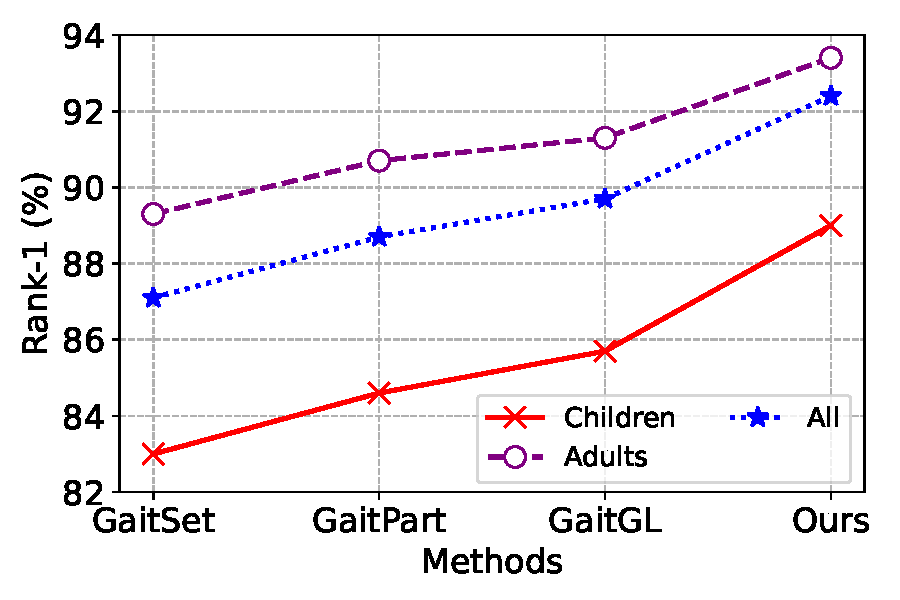
\includegraphics[width=0.80\linewidth]{age.pdf}
% \caption{Age on the OUMVLP dataset.}
% \label{fig:age}
% \end{figure}

\begin{figure}[tb]
\centering
    \subfloat[Average rank-1 accuracy]{
        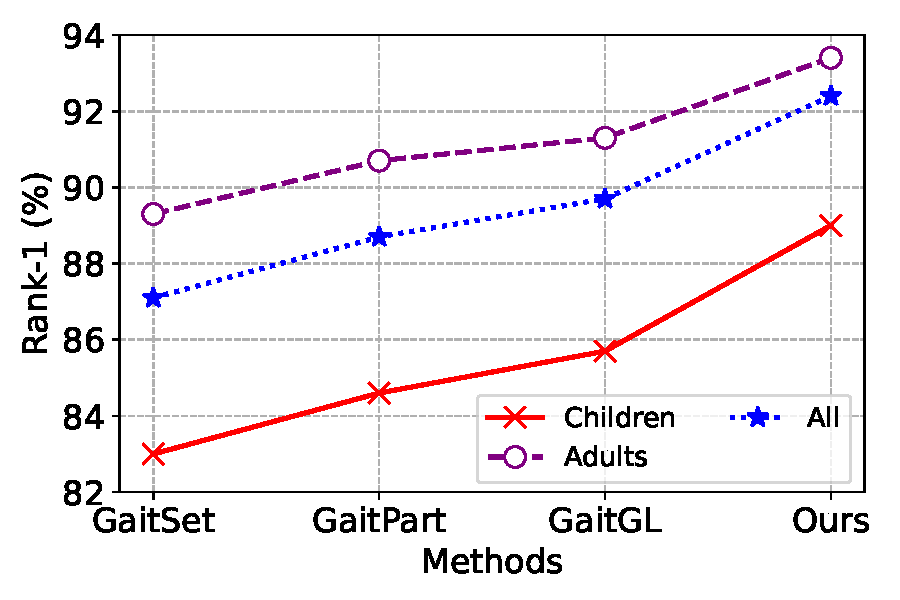
\includegraphics[width=0.61\linewidth]{age.pdf}
        \label{fig:age}
        }
    \subfloat[Age distribution]{
        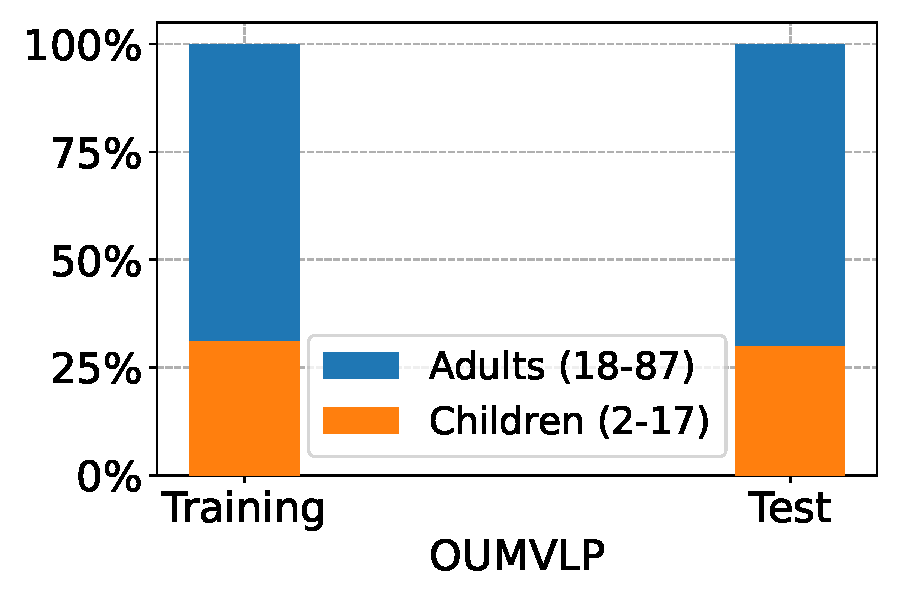
\includegraphics[width=0.35\linewidth]{prob.pdf}
        \label{fig:prob}
        }
    \caption{Cross-age comparison results for the OUMVLP dataset. (a) Average rank-1 accuracy in adults vs children. (b) Distribution of two age groups.}
    \label{fig:cvpr-ou}
\end{figure}

\noindent\textbf{Evaluation on OUMVLP.} To verify the model's generalizability, we conduct experiments on the large-scale OUMVLP dataset.  As shown in Table~\ref{tab:sota-ou}, our approach achieves competitive results in most views. In particular, the proposed method outperforms the second-best method (MetaGait) by an average of 2.5\% under three extreme views, i.e., 0$^{\circ}$, 180$^{\circ}$, and 270$^{\circ}$, resulting in the best mean performance and cross-view stability. In addition, the OUMVLP dataset also provides annotations for the ages of the subjects. To evaluate the impact of age differences on recognition performance, we divided all subjects into two groups: adults (18-87 years old) and children (2-17 years old), as shown in Fig.~\ref{fig:cvpr-ou}\subref{fig:prob}.  Fig.~\ref{fig:cvpr-ou}\subref{fig:age} presents the recognition accuracy based on age. It can be observed that, as adult sequences make up about 70\% of the total sequences, all the compared methods show a bias toward the recognition results of adults. However, compared to other methods, our model effectively improves the accuracy of gait recognition for children, demonstrating the effectiveness of our hierarchical gait representation across ages.



%The recognition accuracy by age is shown in Fig.\ref{fig:age}. It can be seen that, as the adult sequences make up 70\% of the total data volume, the compared methods tend to have better recognition results for adults. However, our method effectively improves the accuracy of gait recognition for children, compared to other methods, demonstrating the applicability of the hierarchical gait representation across ages.




%To verify the generalizability of the model, we conduct experiments on the large-scale OUMVLP dataset. As shown in Table ~\ref{tab:sota-ou}, our approach achieves competitive results in most views. Especially the more extreme view such as $0^{\circ}$ (91.4\%), $180^{\circ}$ (92.7\%), show the advantages. Our method achieves a lower standard deviation than MetaGait, which indicates greater stability to the viewpoint. In addition, as shown in Fig.~\ref{fig:cvpr-ou}\subref{fig:age}, we give the rank-1 accuracy under different age groups \cite{xu2021real}. It can be seen that the accuracy of the children group is lower than that of the adult group. The possible reason for this is that the training set of children (30\%) is less than that of adults (70\%) as is shown in Fig.~\ref{fig:cvpr-ou}\subref{fig:prob}, which affects the ability of the model to fit the gait of children. The better compatibility of our method compared to previous methods is due to the adaptive feature extraction of ARME.


%Notably, there are some probe sequences that have no corresponding sequences in the gallery. Therefore, we discard the invalid probe sequences and present the results in Tab.~\ref{tab:sota-ou-probe}. It is clearly seen that our method outperforms other baselines at all view angles.

\noindent\textbf{Evaluation on GREW and Gait3D.}  Gait3D and GREW are two recently introduced datasets that contain challenging conditions, such as misalignment of the human body and partial occlusion. Tables ~\ref{tab:grew} and ~\ref{tab:res-gait3d} show the results of the comparison between the proposed method and the state-of-the-art methods. Our method shows superior performance in all metrics, indicating its ability to effectively model gait characteristics in realistic scenarios.


%Gait3D and GREW are two recently proposed wild datasets that contain more complex conditions than CASIA-B and OUMVLP, for example, misalignment of the human body and partial occlusion. Tab.~\ref{tab:grew} and Tab.~\ref{tab:res-gait3d} show the results of the comparison between the proposed method and current state-of-the-art methods. The best performance of our method is achieved in all comparison settings, demonstrating the gait modelling capability of our method in realistic scenarios.
\begin{figure}[bt]
  \centering
  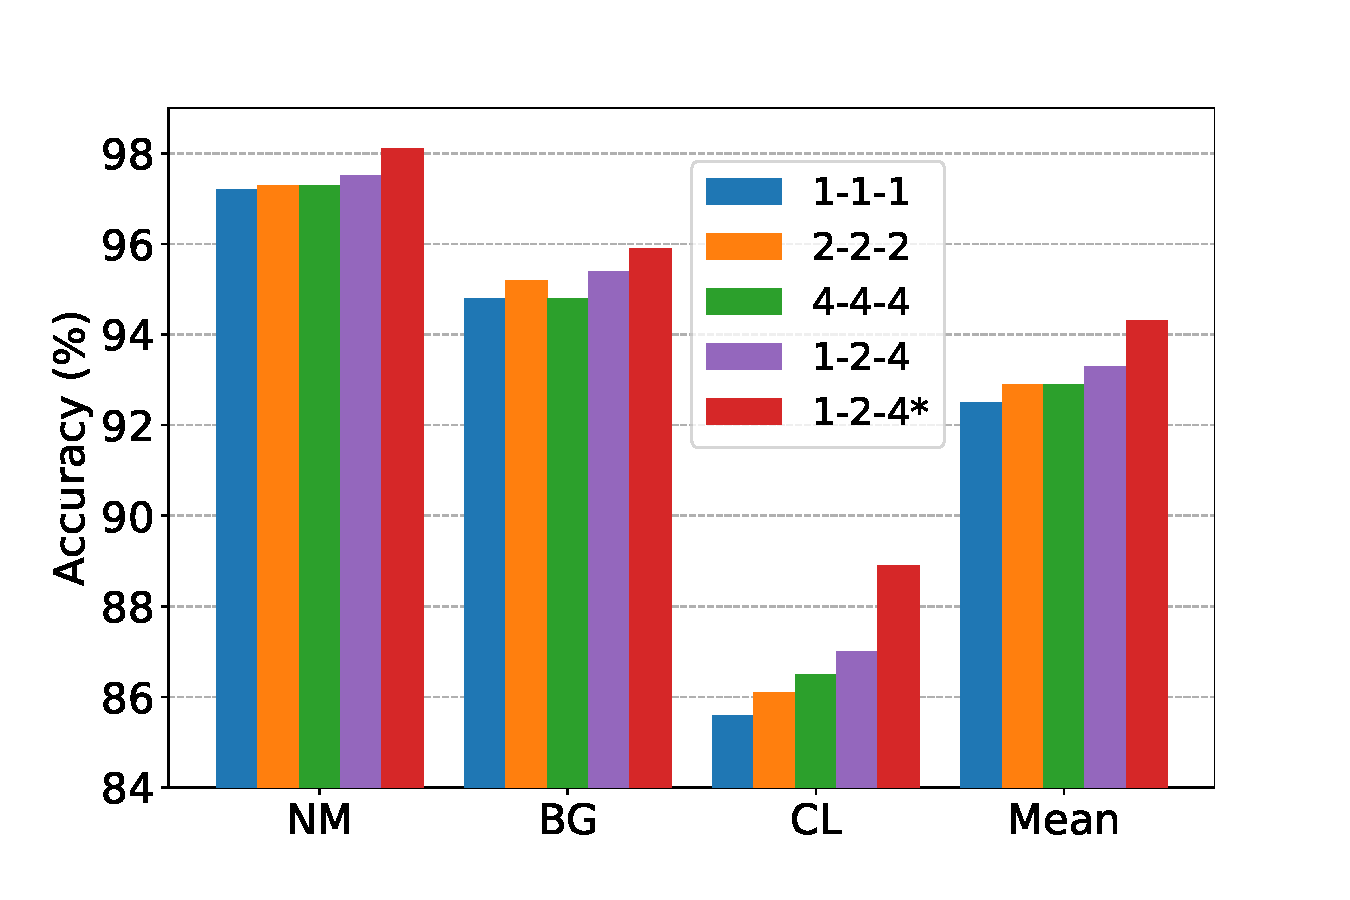
\includegraphics[width=0.87 \linewidth]{hlb.pdf}
\caption{Ablation study on the effectiveness of hierarchical feature extraction on the CASIA-B dataset (best viewed in color).}
\label{fig:hlb-ab}
\end{figure}
\subsection{Ablation Study}
\label{sec:albation}
% In this section, we perform ablation studies to
% verify the contributions of each component in the proposed framework.

\noindent\textbf{Effectiveness of hierarchical feature extraction.} To verify the effectiveness of our hierarchical gait partitioning, we conduct experiment with various grouping strategies. As shown in Table \ref{tab:pcb-str}, this comparison only considers the different settings of the first three layers since a uniform partition is used at layer 4. Specifically, 1-1-1 indicates that the first three levels have the same number of groupings, and they are divided uniformly. 1-2-4* refers to the non-uniform division used in the proposed model. As shown in Fig.~\ref{fig:hlb-ab}, the hierarchical feature extraction setting, e.g., 1-2-4, outperforms the other non-hierarchical approaches. A further mean performance improvement of 1.0\% is achieved when the motion relationships between different body regions, i.e., 1-2-4*, are considered.






%To verify the effectiveness of the hierarchy, we conducted five groups of controlled experiments with different experimental settings, as shown in Fig.~\ref{fig:hlb-ab}. Where 1-1-1 denotes the number of groups $\left\{K_l\right\}_{l=1}^{l=3}$ of the three-level uniform version of ARME and 1-2-4* denotes the ARME of our method (i.e., the non-uniform version of ARME). 1) The results of the first four sets of experiments show that experiments 1-2-4 have the best mean accuracy (93.3\%), indicating that incremental splits according to hierarchy can better represent the hierarchical relationship of gait features and thus enhance the fine-graininess of local features. 2) The last two experiments show that the stacked non-uniform version of ARME has the best mean accuracy (94.3\%), especially in the CL condition (88.9\%), which indicates the effectiveness of the ARME module and verifies the adaptability of the non-uniform hierarchical representation to hard-to-identify samples.


% \noindent\textbf{Effectiveness of FTA.} As shown in Tab.~\ref{tab:mma-ab}, we design five groups of control experiments (numbered a, b, c, d and e). 1) By comparing and contrasting experiments a, b and c, experiment c outperformed either experiment a or b, indicating the effectiveness of the adaptive
%  multi-scale temporal fusion mechanism of FTA. We believe this is due to the FTA capturing discriminative temporal information enhancing the feature representation. 2) By comparing experiments c, d and e use different pooling operators respectively, where conv is convolution pooling with stride ($3\times1\times1$). It can be seen that the choice of pooling operator is crucial for FTA. Experiment c results achieve best, indicating that max pooling helps FTA to eliminate similar frame features of local clips.



% 1) Notice that experiment a does not perform temporal downsampling, i.e., the experiments using the MMA module (b, c, and d) all obtain better mean accuracies than experiment a, which validates the effectiveness of the MMA. Compressing local clips serves to eliminate redundant information.
%CASIA-B上MMA模块的有效性研究。结果是11个视角和三种行走条件的平均rank-1准确度，不包括相同视角的情况。PKS表示时间池化核大小，K3表示时间池化核大小为3，以此类推。
% \begin{table}[htbp]
%   \centering
%   \caption{Ablation study of the effectiveness of the MMA module on CASIA-B. The results are the average rank-1 accuracy. K3 and K5 denote the kernel sizes of 3 and 5 for temporal pooling, respectively.}
%     \begin{tabular}{ccc|cccc}
%     \toprule
%     \multirow{2}[1]{*}{Setting} & \multicolumn{2}{c|}{FP} & \multicolumn{4}{c}{accuracy} \\
% \cline{2-7}          & K3    & K5     & NM    & BG    & CL    & Mean \\
%     \hline
%     a     &      &        & \textbf{97.8}  & 95.3  & 85.9  & 93.0  \\
%     \hline

%     b     & \checkmark     &        & 97.7  & 95.1  & 86.4  & 93.1  \\
%     % \hline
%     c     &       & \checkmark        & 97.7  & \textbf{95.4}  & 87.1  & 93.4  \\
%     % \hline
%     % c     &       &         & 97.5  & 94.9  & 86.6  & 93.0  \\
%     \hline
%     % d     &   $-$    & $-$       & 97.6  & 95.2  & 86.8  & 93.2  \\
%     % \hline
%     % e     & \checkmark     &           & \textbf{97.8} & \textbf{95.7} & 86.9  & 93.5  \\
%     % \hline
%     d     & \checkmark     & \checkmark    & \textbf{97.8} & \textbf{95.4}  & \textbf{87.5} & \textbf{93.6} \\
%     \bottomrule
%     \end{tabular}%
%   \label{tab:mma-ab}%
% \end{table}%

% Table generated by Excel2LaTeX from sheet 'Sheet1'
% \begin{table}[htbp]
%   \centering
%   \caption{Ablation study of the effectiveness of FTA on CASIA-B in terms of average rank-1 accuracy.}
%   \setlength{\tabcolsep}{2mm}{
%     \begin{tabular}{c|cc|c|ccc}
%     \toprule
%     \multirow{2}[1]{*}{Setting} & \multicolumn{2}{c|}{Kernel Size} & \multirow{2}[1]{*}{Operator} & \multicolumn{3}{c}{Accuracy} \\
% \cline{2-3}\cline{5-7}          & 3     & \multicolumn{1}{c|}{5}     &       & \multicolumn{1}{c}{NM}    & BG    & CL \\
%     \hline
%     a     & \checkmark     &       & max   & 97.7  & 95.3  & 87.5 \\
%     % \midrule
%     b     &       & \checkmark     & max   & 97.7  & 95.2  & 87.2 \\
%     % \midrule
%     c     & \checkmark     & \checkmark     & max   & \textbf{98.1}  & \textbf{95.9}  & \textbf{88.9} \\
%     % \hline
%     d     & \checkmark     & \checkmark     & avg   & 97.7 & 95.6 & 87.9 \\
%     % \hline
%     e     & \checkmark     & \checkmark     & conv  &   96.2    &   92.4    & 80.5 \\
%     \bottomrule
%     \end{tabular}%
%     }
%   \label{tab:addlabel}%
%   \label{tab:mma-ab}%
% \end{table}%

 \noindent\textbf{Effectiveness of ARME, ASTP, and FTA.} The results of the ablation experiments for ARME, ASTP, and FTA are shown in Tab.~\ref{tab:impact} The results indicate that the ARME module significantly contributes to the improvement of the recognition accuracy, with an average improvement of 1.1\% compared to the baseline model (non-grouping version of ARME). The mean accuracy is further improved by 1.3\% when the ASTP module is integrated and multi-scale fusion is utilized in FTA. These results demonstrate the effectiveness and complementarity of the three modules in the proposed gait recognition framework.


 %Tab.~\ref{tab:impact} demonstrates the impact of ASTP and FTA on the accuracy of our method. ASTP-free means feature aggregation using TP+GeM \cite{lin2021gait,lin2021gaitmask} after the last level of ARME. 1) Using only ARME to model gait, 97.8\% accuracy is achieved at NM, demonstrating the superiority of ARME adaptive modelling of motion features. 2) Compared to experiment a, there is an improvement in CL for both experiment b (+1.1\%) and experiment e (+1.6\%), indicating that ASTP and FTA have a positive effect on the representation discriminant enhancement. 3) In experiment f, the best results are achieved by applying both ASTP and FTA, indicating that ASTP and FTA are complementary. 4) By comparing experiments c, d and f, which demonstrates the validity of the FTA multi-scale.
% Table generated by Excel2LaTeX from sheet 'Sheet1'
% \begin{table}[htbp]
%   \centering
%   \setlength{\abovecaptionskip}{0cm}  %段前
% \setlength{\belowcaptionskip}{-0.2cm} %段后
%   \caption{Ablation study of the impact of spatio-temporal aggregation on CASIA-B in terms of average rank-1 accuracy. $\dagger$ and $\ddagger$ denote the temporal kernel sizes of 3 and 5 for FTA, respectively.}
%   \setlength{\tabcolsep}{1mm}{
%     \begin{tabular}{c|ccc|cccc}
%     \toprule
%     Setting & ARME  & ASTP  & FTA   & NM    & BG    & CL  & Mean  \\
%     \hline
%     a     & \checkmark &       &       & 97.8  & 95.3  & 85.9 & 93.0 \\
%     % \midrule
%     b     & \checkmark & \checkmark &  & 97.8& 95.4 &   87.0 & 93.4   \\
%     % \midrule
%     c     & \checkmark &       & \checkmark & 97.8  & 95.4  & 87.5 & 93.6   \\
%     % \midrule
%     d     & \checkmark & \checkmark & \checkmark & \textbf{98.1}  & \textbf{95.9}  & \textbf{88.9} & \textbf{94.3}  \\
%     e     & \checkmark & \checkmark & $\dagger$ & 97.7  & 95.3  & 87.5 & 93.5  \\
%     f     & \checkmark & \checkmark & $\ddagger$  & 97.7  & 95.2  & 87.2 & 93.4  \\
%     \bottomrule
%     \end{tabular}%
%     }
%   \label{tab:impact}%
% \end{table}%
% Table generated by Excel2LaTeX from sheet 'Sheet1'


\subsection{Trade-off between accuracy and efficiency}
\label{sec:trade-off}

 \begin{table}[tb]
  \centering
    \setlength{\abovecaptionskip}{0cm}  %段前
\setlength{\belowcaptionskip}{-0.2cm} %段后
  \caption{Ablation study on the effectiveness of ARME, ASTP, and FTA modules in terms of average rank-1 accuracy on the CASIA-B dataset.}
  \resizebox{\linewidth}{!}{
    \begin{tabular}{c|cc|cc|ccc|c}
    \toprule
    \multirow{2}[1]{*}{Setting} & \multirow{2}[1]{*}{ARME} & \multirow{2}[1]{*}{ASTP} & \multicolumn{2}{|c|}{FTA} & \multirow{2}[1]{*}{NM} & \multirow{2}[1]{*}{BG} & \multirow{2}[1]{*}{CL} & \multirow{2}[1]{*} {Mean} \\
\cline{4-5}          &       &       &  \multicolumn{1}{|c|}3     & 5     &       &       &       &  \\
    \hline
     a     &      &       &       &       & 97.0  & 94.5  & 84.2  & 91.9 \\
    b     & \checkmark     &       &       &       & 97.8  & 95.3  & 85.9  & 93.0 \\

    % \midrule
    c     & \checkmark     & \checkmark     &  &   & 97.8 & 95.4 & 87.0 & 93.4 \\
    d     & \checkmark     & \checkmark     & \checkmark     &       & 97.7  & 95.3  & 87.5  & 93.5 \\
    e     & \checkmark     & \checkmark     &       & \checkmark     & 97.7  & 95.2  & 87.2  & 93.4 \\
    % \midrule
    f     & \checkmark     &       & \checkmark     & \checkmark     & 97.8  & 95.4  & 87.5  & 93.6 \\
    % \midrule
    g     & \checkmark     & \checkmark     & \checkmark     & \checkmark     & \textbf{98.1}  & \textbf{95.9}  & \textbf{88.9}  & \textbf{94.3} \\
    % \midrule

    % \hline

    \bottomrule
    \end{tabular}%
    }
  \label{tab:impact}%
\end{table}%
In this subsection, we evaluate the relationship between accuracy and efficiency for each compared method. As shown in Fig.~\ref{fig:trade-off4}, the 3D convolution-based approaches, such as GaitGL \cite{lin2021gait}, 3D Local \cite{huang20213d}, LagrangeGait \cite{chai2022lagrange} and MetaGait \cite{dou2022metagait}, outperform the 2D convolution-based methods, like GaitSet \cite{chao2019gaitset} and GaitPart \cite{fan2020gaitpart}, in terms of accuracy, but at the cost of a significant increase in FLOPs (floating point operations). Our approach has a better trade-off between accuracy and efficiency.  The main reason is that the proposed hierarchical learning architecture can extract multi-level motion features while reducing the number of 3D convolutions. More experimental results and ablation analysis are provided in the \textsl{supplementary material}.

\begin{figure}[tb]
  \centering
  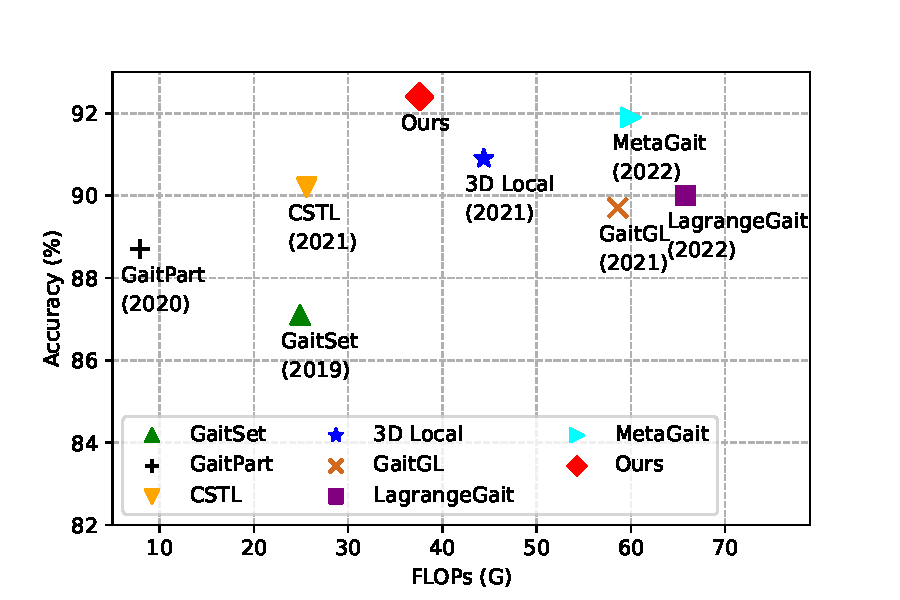
\includegraphics[width=0.91\linewidth]{trade-off4_.pdf}
\caption{The trade-off between accuracy and FLOPs of our method and other comparison methods on the OUMVLP dataset.}
\label{fig:trade-off4}
\end{figure}

%In addition, more ablation experiments are given in \textsl{supplementary material}.






%In this subsection, we evaluate the relationship between accuracy and efficiency for each compared method. As illustrated in Fig.~\ref{fig:trade-off4}, compared to the 2D convolution-based methods, such as GaitSet \cite{chao2019gaitset} and GaitPart \cite{fan2020gaitpart}, the 3D convolution-based approaches such as GaitGL \cite{lin2021gait}, 3D Local \cite{huang20213d}, LagrangeGait \cite{chai2022lagrange} and MetaGait \cite{dou2022metagait} achieve better performance, but at the cost of a significant increase in the number of FLOPs (floating point operations). Our approach has a better trade-off between accuracy and efficiency. The main reason is that the proposed hierarchical-based learning architecture could extract multi-level motion features while reducing the number of 3D convolutions and maintaining the simplicity of the network structure. In addition, More ablation experiments are given in the \textsl{supplementary material}.
% In addition, we analyze the relationship between the number of parameters and the accuracy of the models on the CASIA-B and OUMVLP datasets. More detail can be found in the supplementary materials.


%achieve better performances, but at the cost of a significant increase in the number of FlOPs (floating point operations). Moreover, the number of branches in the network on feature extract also influences efficiency. For example, GaitGL \cite{lin2021gait} (two branches), MetaGait \cite{dou2022metagait} (two branches), and LagrangeGait  \cite{chai2022lagrange} (three branches) require much more FLOPs than 3D Local \cite{huang20213d}  (single branch).


% \subsection{Visualization}
% \label{sec:vis}

% \begin{figure}[t!]
% \centering
%     % \begin{subfigure}[t]{0.36\linewidth}
%     %        \centering
%     %        \includegraphics[width=1.0\linewidth]{vis1.pdf}
%     % \caption{Ours after ARME2}
%     % \label{fig:vis1}
%     % \end{subfigure}
%     \subfloat[Body parts]{
%         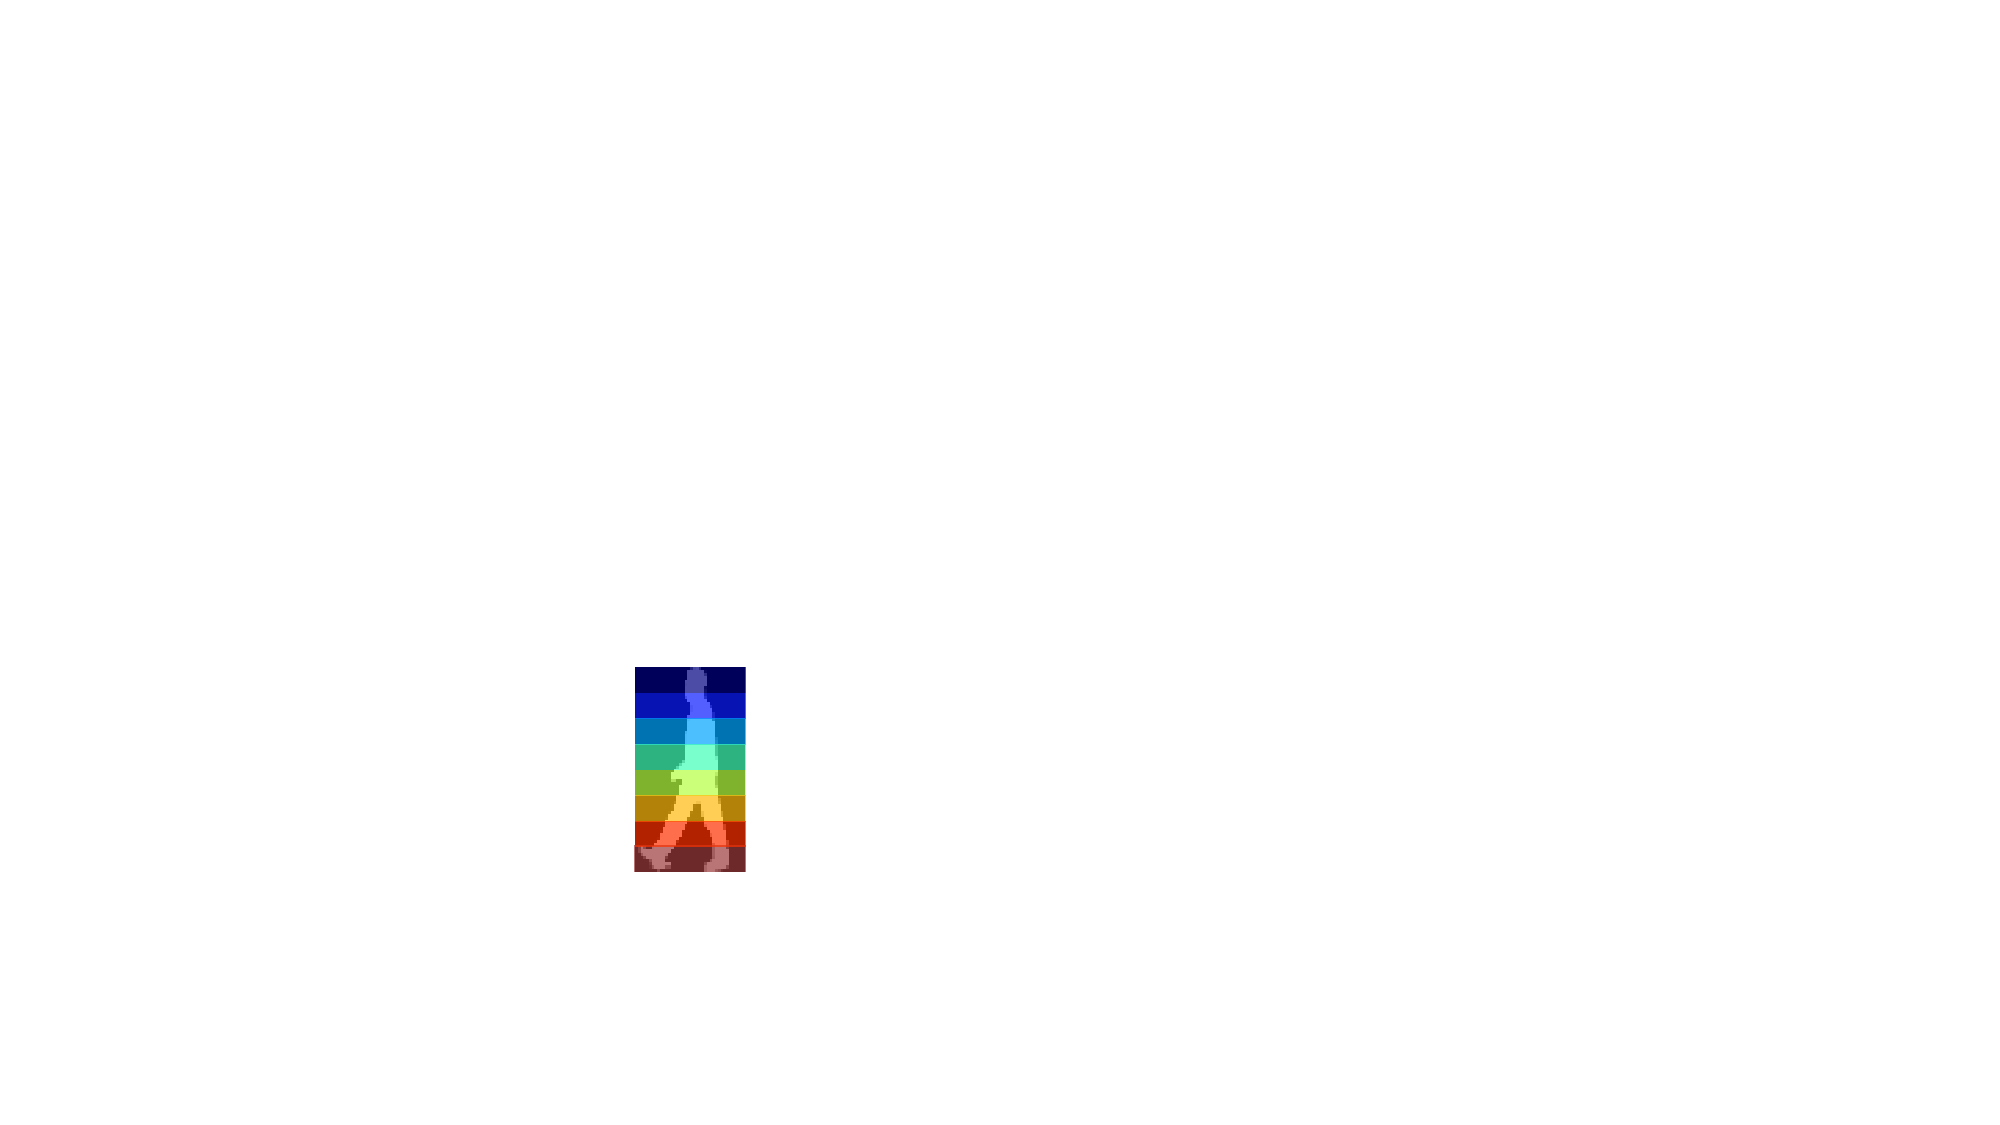
\includegraphics[width=0.16\linewidth]{vis3.pdf}
%         \label{fig:vis3}
%         }
%     % \begin{subfigure}[t]{0.20\linewidth}
%     %         \centering
%     %         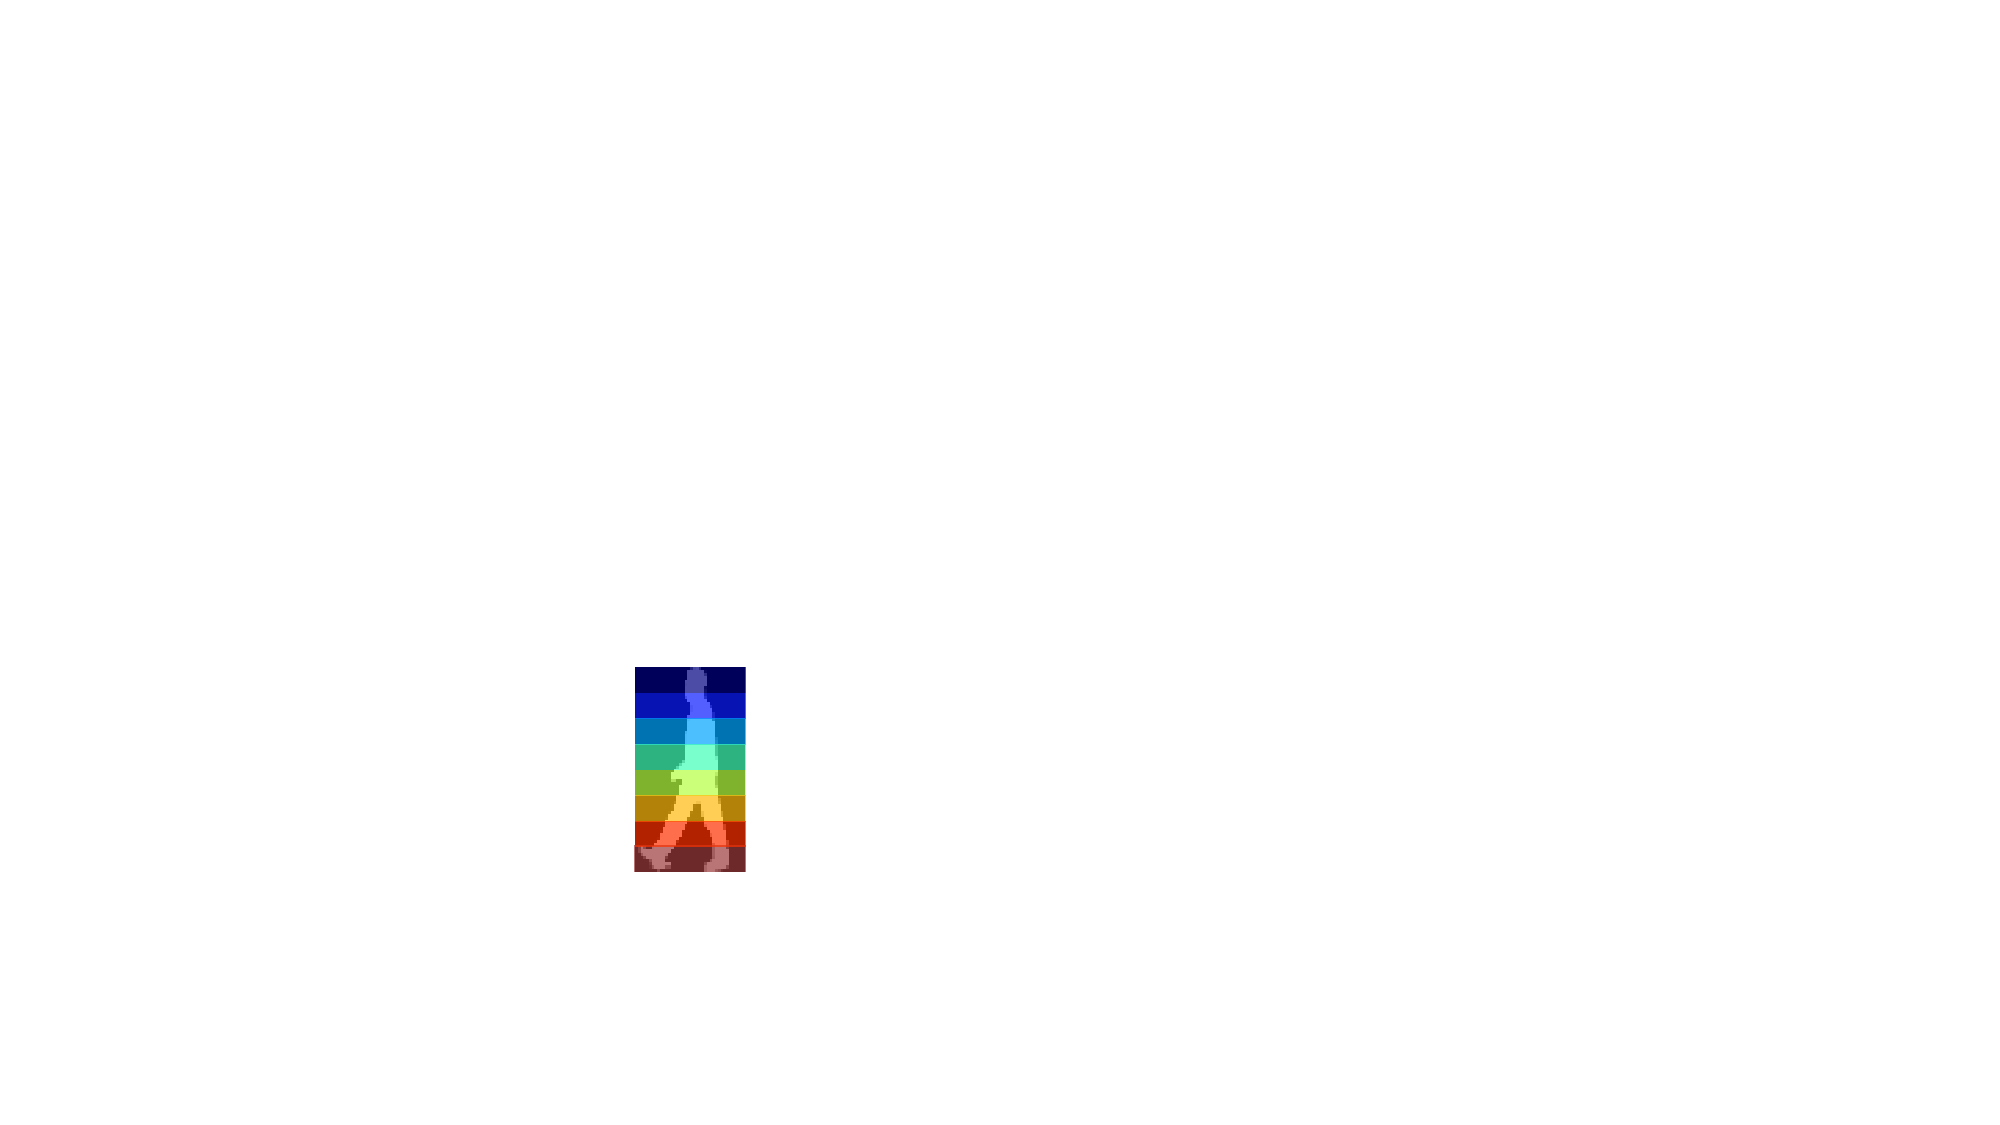
\includegraphics[width=0.8\linewidth]{vis3.pdf}
%     % \caption{Body parts}
%     % \label{fig:vis3}
%     % \end{subfigure}
%     % \begin{subfigure}[t]{0.36\linewidth}
%     %         \centering
%     %         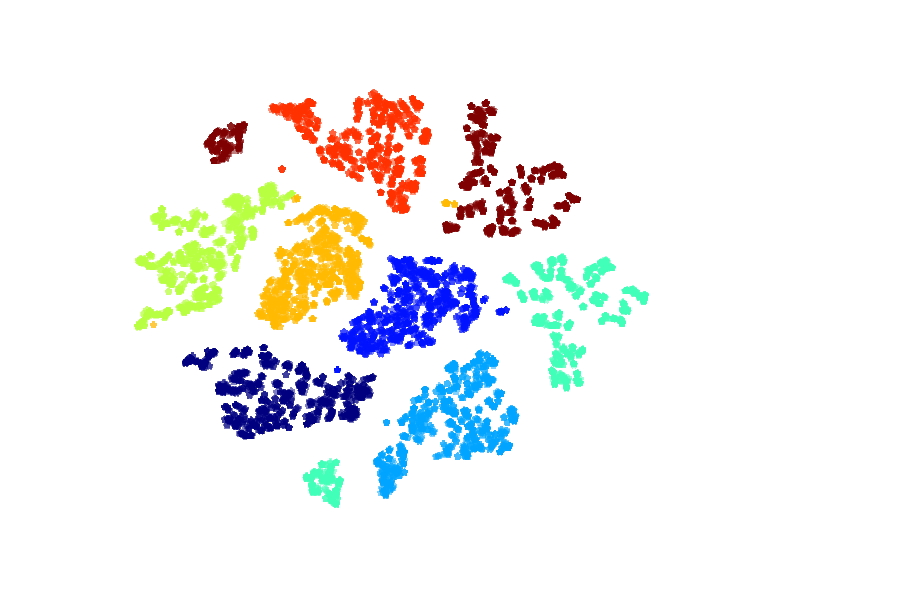
\includegraphics[width=1.0\linewidth]{vis4.pdf}
%     % \caption{GaitGL \cite{lin2021gait}}
%     % \label{fig:vis4}
%     \subfloat[GaitGL \cite{lin2021gait}]{
%         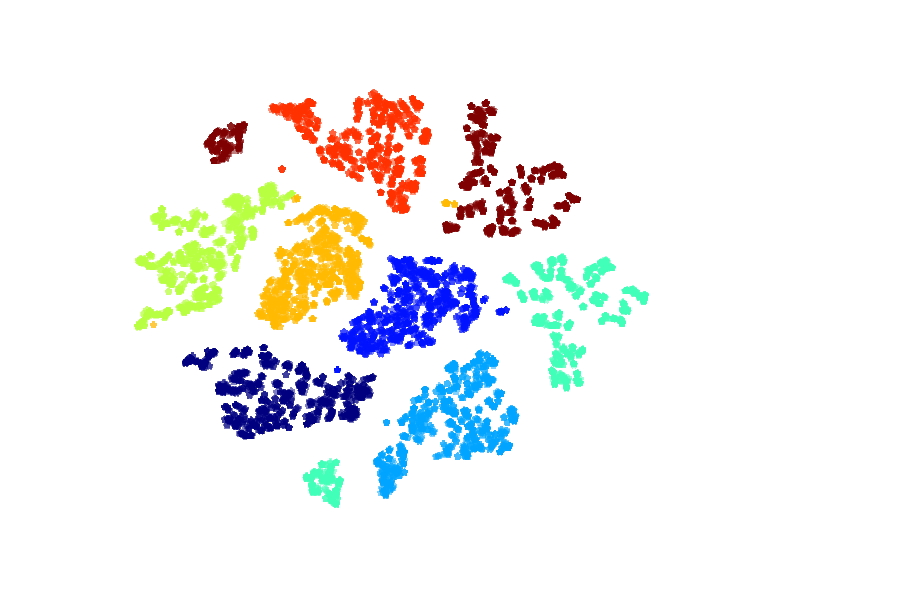
\includegraphics[width=0.36\linewidth]{vis4.pdf}
%         \label{fig:vis4}
%         }
%     % \end{subfigure}
%     % \begin{subfigure}[t]{0.36\linewidth}
%     %         \centering
%     %          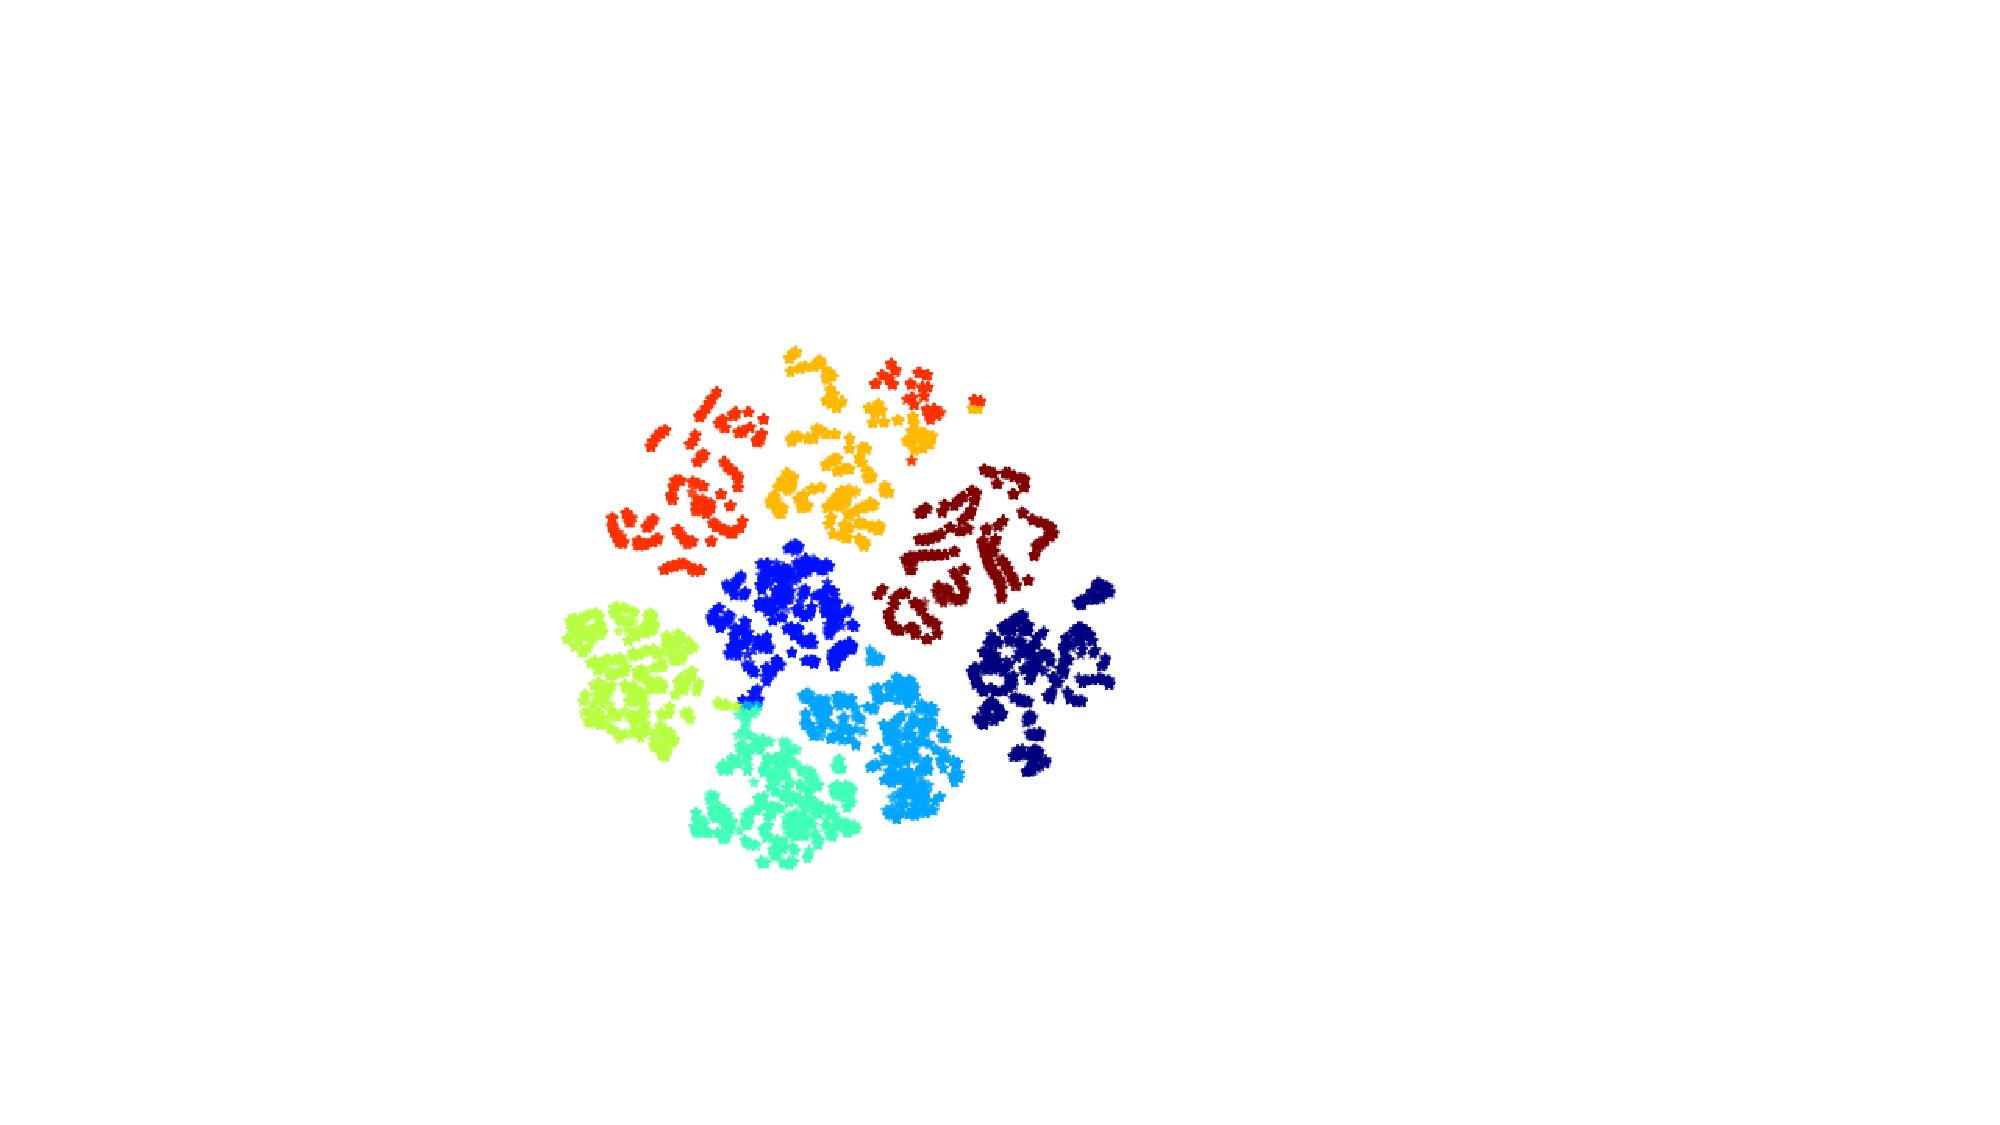
\includegraphics[width=1.0\linewidth]{vis2.pdf}
%     % \caption{Ours}
%     % \label{fig:vis2}
%     % \end{subfigure}
%     \subfloat[Ours]{
%         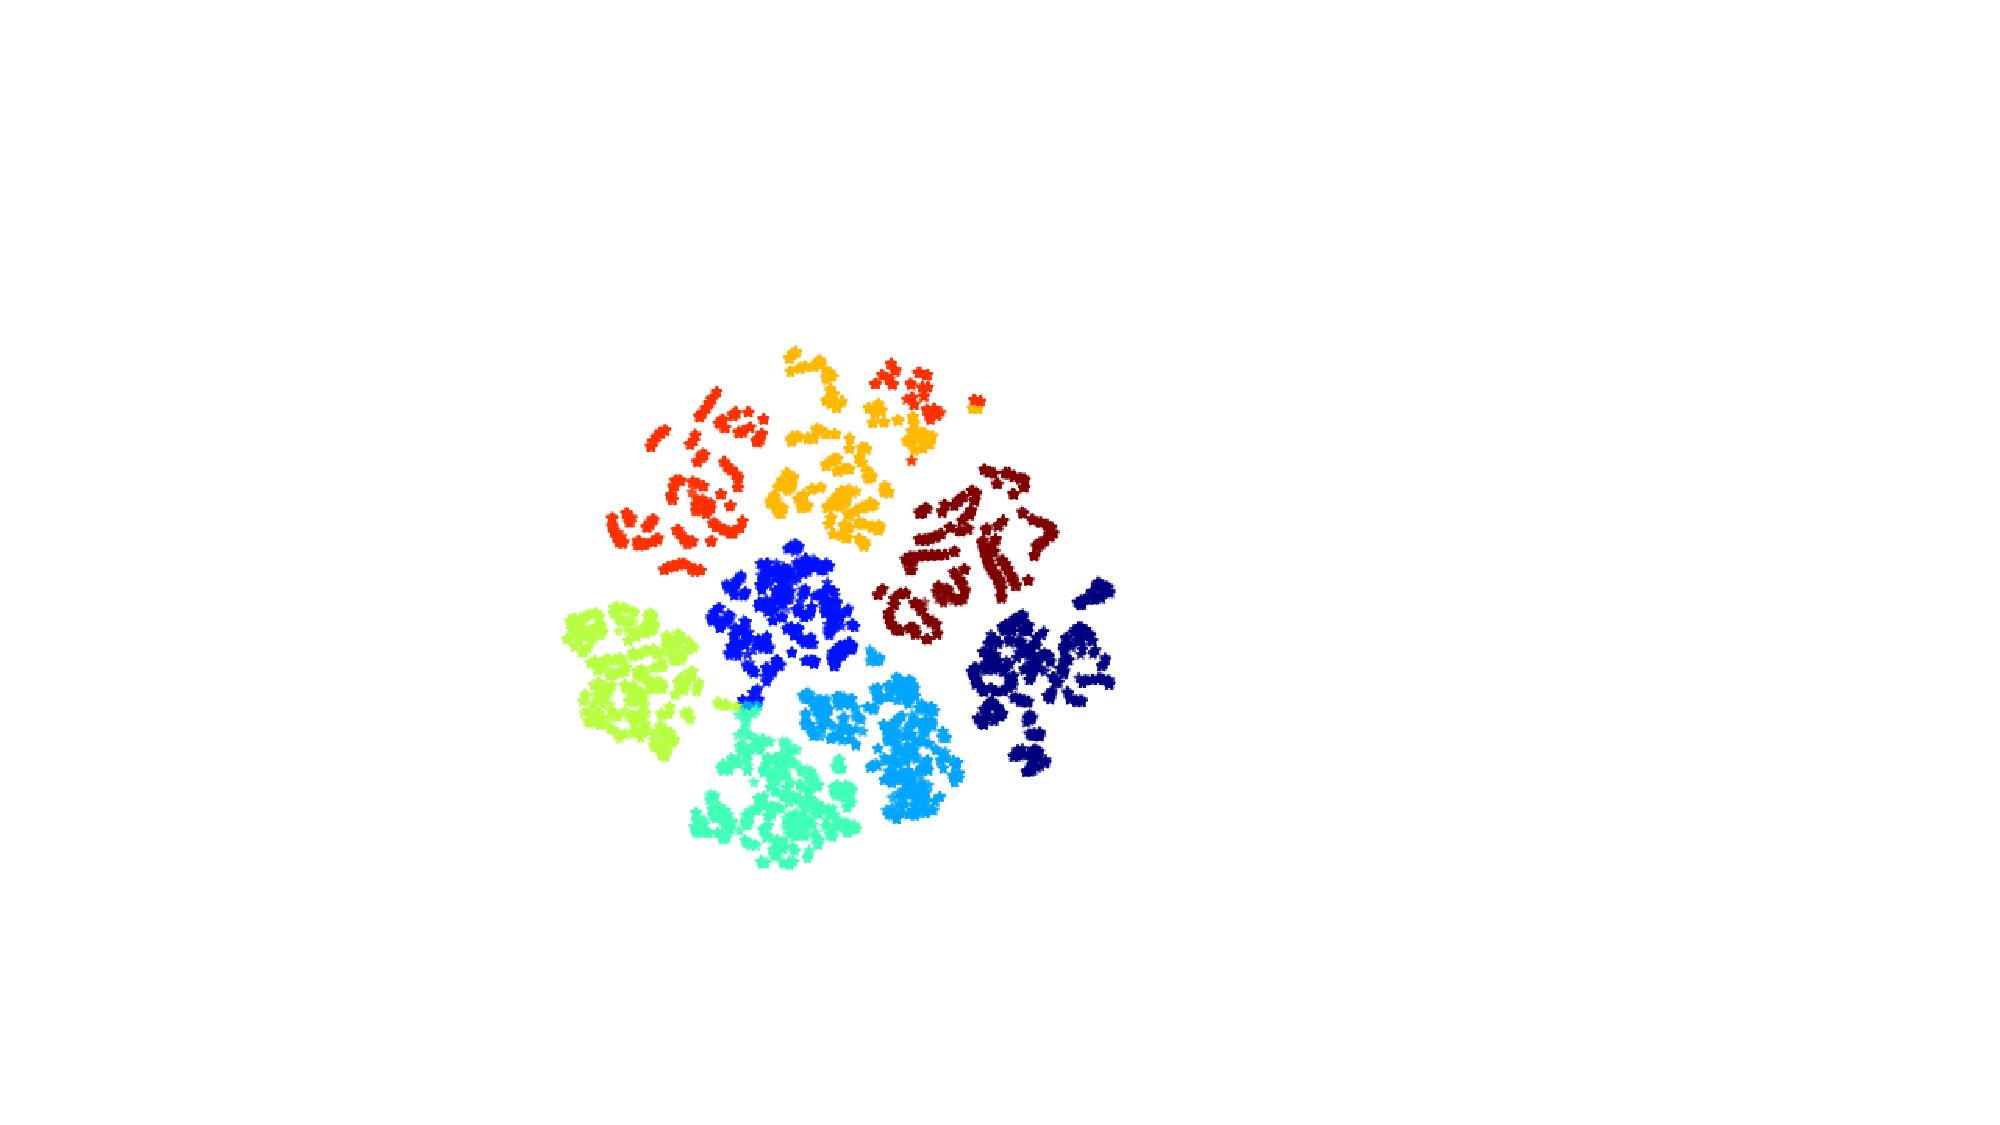
\includegraphics[width=0.36\linewidth]{vis2.pdf}
%         \label{fig:vis2}
%         }
%     % \\
%     % \begin{subfigure}[t]{0.36\linewidth}
%     %         \centering
%     %         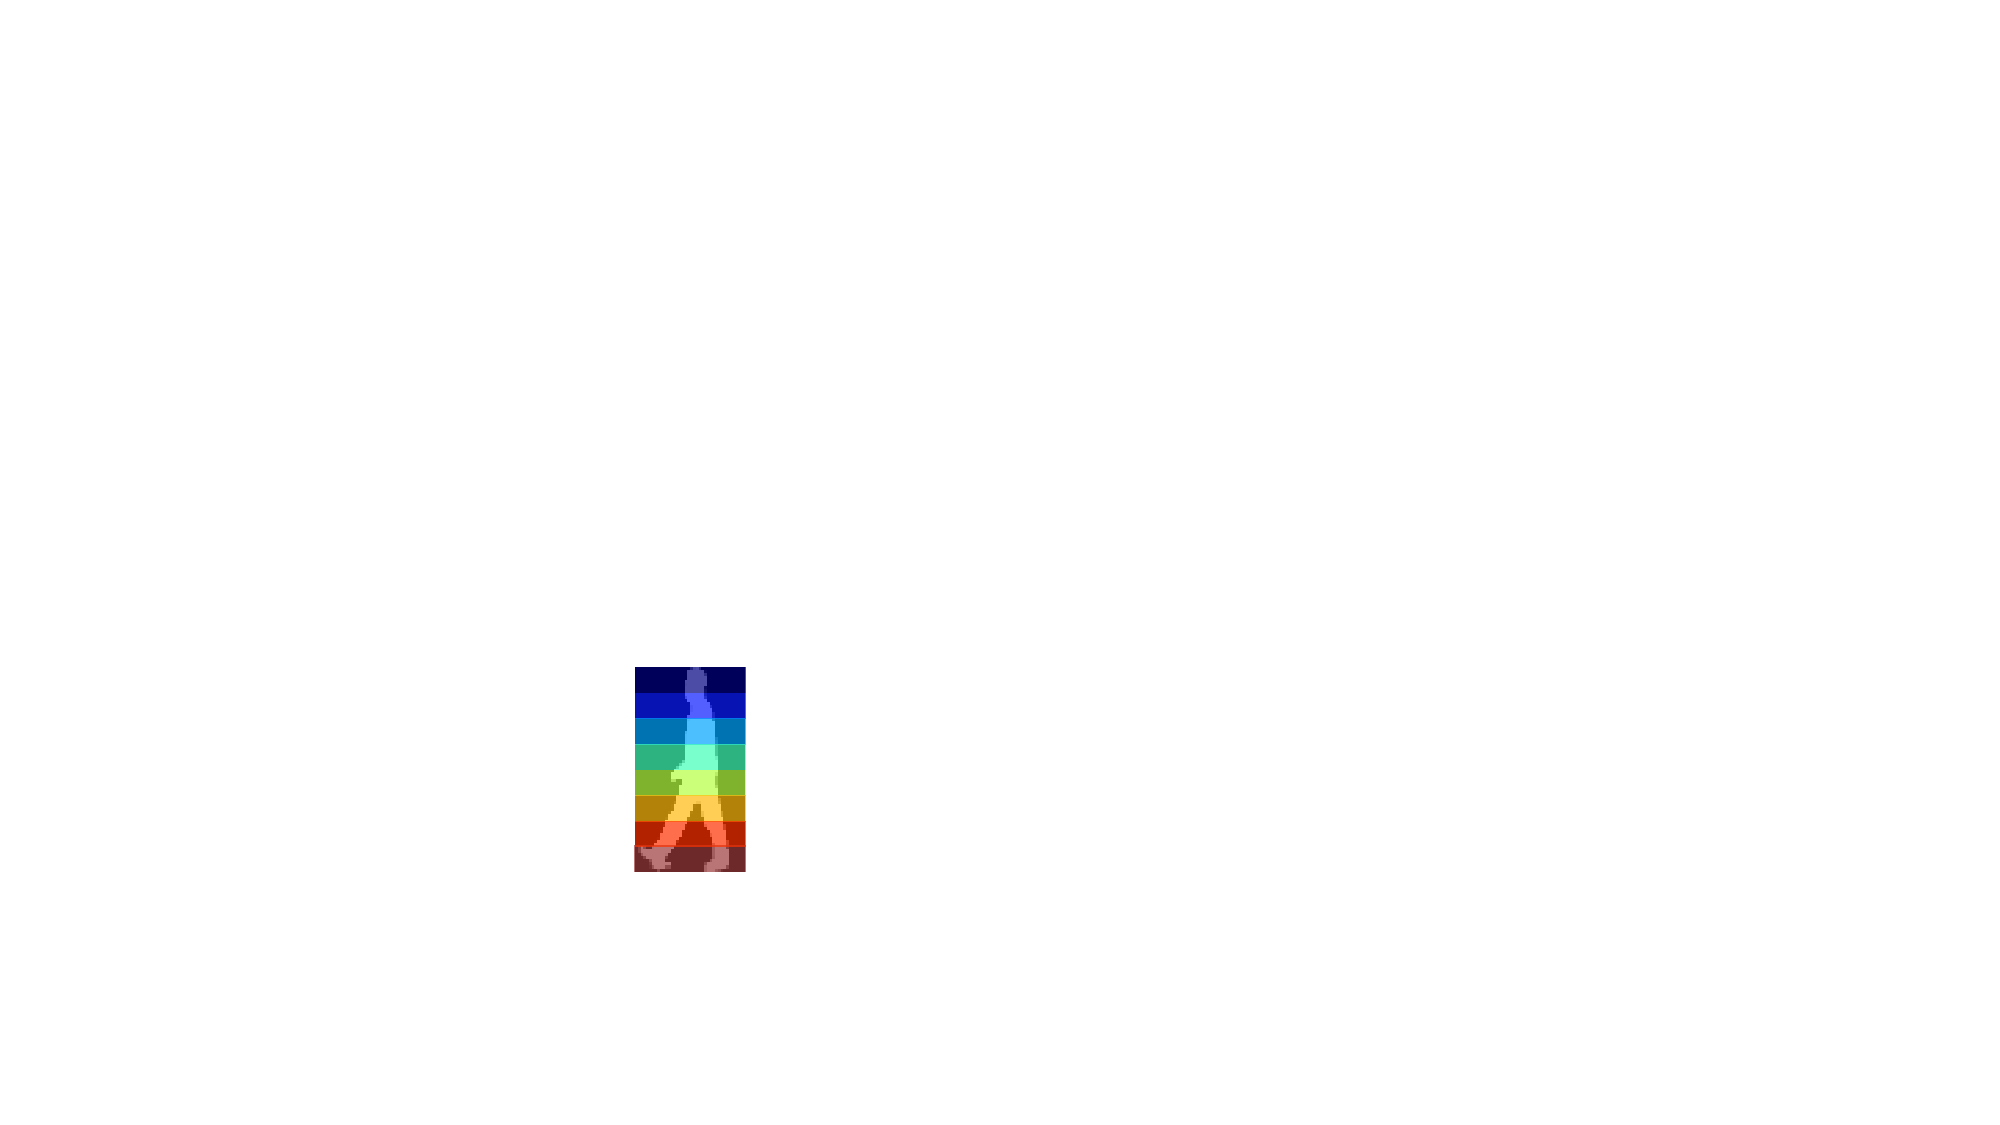
\includegraphics[width=1.0\linewidth]{vis3.pdf}
%     % \caption{GaitPart after block2}
%     % \label{fig:vis3}
%     % \end{subfigure}

%     \caption{Visualizations of different body parts. A horizontal slice of feature maps is shown in (a).
%     Each color denotes a separable part.  Comparisons of the part-based features between GaitGL and our method are shown in (b) and (c), respectively.}
%     \label{fig:vis-map}
% \end{figure}

% In gait recognition, it has been a common practice to horizontally split the feature map into stripes for part-based learning \cite{fan2020gaitpart,lin2021gait,lin2021gaitmask,chai2022lagrange}. To verify the effectiveness of the hierarchical partitioning proposed in this paper, we first select ten subjects in the CASIA-B datasets and then visualize the different local parts via t-SNE \cite{van2008visualizing}. Specifically, as shown in Fig. \ref{fig:vis3}, the feature maps output by the last modules of GaitGL \cite{lin2021gait} and HSTL are uniformly split into eight stripes, and their features are visualized Fig. \ref{fig:vis2} and \ref{fig:vis4} respectively. Clearly, in GaitGL, it is harder to distinguish the different body parts, which decreases the discriminability of the global gait representation. In contrast, our method is able to refine the boundaries of the body parts, which could provide high-quality part-specific representation for gait recognition.

% \subsection{Limitations}
% In HSTL, some 3D convolutions are employed to extract spatio-temporal information. Although the number of 3D convolutions is reduced by sharing the same operator between adjacent body parts, the number of FLOPs is still increased considerably compared to 2D convolution-based methods (e.g., GaitSet\cite{chao2019gaitset} and GaitPart \cite{fan2020gaitpart}). In addition, HSTL uses a naive part localization strategy, uniform splitting, to obtain the body hierarchy. Therefore, it is necessary to design adaptive and lightweight mechanisms for exploring gait motion characteristics.

\section{Conclusion}
\label{sec:conclu}
%本文提出了一个新的步态识别框架，GaitPST，它层次化的提取部分序列的局部运动特征。提出了层次学习块来建模部分序列的时空表征。MMA模块通过自适应的选择池化感受野来压缩局部剪辑进而聚合时间信息。此外，我们还讨论了模型性能与模型参数量、模型计算复杂度的关系。最后，我们在两个公共数据集上进行了广泛的实验以验证GaitPST的有效性。
This paper presents a hierarchical spatio-temporal representation learning (HSTL) framework for gait recognition. HSTL stacks multiple adaptive region-based motion extractors (ARMEs) and learns walking patterns in a coarse-to-fine manner. An adaptive spatio-temporal pooling (ASTP) module is proposed to perform hierarchical feature mapping for the output of each level of ARME. Additionally, a frame-level temporal aggregation module (FTA) is designed to compress local clips by fusing temporal information. The effectiveness of the proposed HSTL framework is demonstrated through extensive experiments conducted on four public datasets (CASIA-B, OUMVLP, GREW, and Gait3D).

\section*{Acknowledgements}
This work was supported by the National Natural Science Foundation of China (Grant Nos. 61972132, 62106065) and the Research Project for Self-cultivating Talents at Hebei Agricultural University (Grant No. PY201810).

% \section{Final copy}

% You must include your signed IEEE copyright release form when you submit
% your finished paper. We MUST have this form before your paper can be
% published in the proceedings.

\clearpage
{\small
\bibliographystyle{ieee_fullname}
\bibliography{hstl_final_paper}
}

\end{document}